\documentclass[12pt,]{article}
%\usepackage{lmodern}  Melissa removed to deal with font rendering issue
\usepackage{amssymb,amsmath}
\usepackage{ifxetex,ifluatex}
\usepackage{fixltx2e} % provides \textsubscript

%Melissa removed the following section to deal with font rendering issue
%\ifnum 0\ifxetex 1\fi\ifluatex 1\fi=0 % if pdftex
%  \usepackage[T1]{fontenc}
%  \usepackage[utf8]{inputenc}
%%\else % if luatex or xelatex
%  \ifxetex
%    \usepackage{mathspec}
%  \else
%    \usepackage{fontspec}
%  \fi
%  \defaultfontfeatures{Ligatures=TeX,Scale=MatchLowercase}
%  \newcommand{\euro}{€}
%%%%%%\fi

% use upquote if available, for straight quotes in verbatim environments
\IfFileExists{upquote.sty}{\usepackage{upquote}}{}
% use microtype if available
\IfFileExists{microtype.sty}{%
\usepackage{microtype}
\UseMicrotypeSet[protrusion]{basicmath} % disable protrusion for tt fonts
}{}
\usepackage[margin=1in]{geometry}
\usepackage{hyperref}
\PassOptionsToPackage{usenames,dvipsnames}{color} % color is loaded by hyperref
\hypersetup{unicode=true,
            pdftitle={Status of Pacific ocean perch (Sebastes alutus) along the U.S. west coast in 2017},
            pdfborder={0 0 0},
            breaklinks=true}
\urlstyle{same}  % don't use monospace font for urls
\usepackage{graphicx,grffile}
\makeatletter
\def\maxwidth{\ifdim\Gin@nat@width>\linewidth\linewidth\else\Gin@nat@width\fi}
\def\maxheight{\ifdim\Gin@nat@height>\textheight\textheight\else\Gin@nat@height\fi}
\makeatother
% Scale images if necessary, so that they will not overflow the page
% margins by default, and it is still possible to overwrite the defaults
% using explicit options in \includegraphics[width, height, ...]{}
\setkeys{Gin}{width=\maxwidth,height=\maxheight,keepaspectratio}
\setlength{\parindent}{0pt}
\setlength{\parskip}{6pt plus 2pt minus 1pt}
\setlength{\emergencystretch}{3em}  % prevent overfull lines
\providecommand{\tightlist}{%
  \setlength{\itemsep}{0pt}\setlength{\parskip}{0pt}}
\setcounter{secnumdepth}{5}

%%% Use protect on footnotes to avoid problems with footnotes in titles
\let\rmarkdownfootnote\footnote%
\def\footnote{\protect\rmarkdownfootnote}

%%% Change title format to be more compact
\usepackage{titling}

% Create subtitle command for use in maketitle
\newcommand{\subtitle}[1]{
  \posttitle{
    \begin{center}\large#1\end{center}
    }
}

\setlength{\droptitle}{-2em}
  \title{Status of Pacific ocean perch (\emph{Sebastes alutus}) along the U.S.
west coast in 2017}
  \pretitle{\vspace{\droptitle}\centering\huge}
  \posttitle{\par}
  \author{}
  \preauthor{}\postauthor{}
  \date{}
  \predate{}\postdate{}


% This file contains all of the LaTeX packages you may need to compile the document
% Documentation for each package can be found onlines
\usepackage{tabularx}                                             % table environment providing flexibility
\usepackage{caption}                                              % for creating captions  
\usepackage{longtable}                                            % allows tables to span multiple pages
\usepackage{rotating}                                             % allows for sideways tables
\usepackage{float}                                                % floating environments; may not need in rmarkdown
\usepackage{placeins}                                             % keeps floats from moving
\usepackage{indentfirst}                                          % indents first paragraph of a section
\usepackage{mdwtab}                                               % continued float multi-page figure
\usepackage{enumerate}                                            % create lists
\usepackage{hyperref}                                             % highlight cross references
\hypersetup{colorlinks=true, urlcolor=blue, linktoc=page, linkcolor=blue, citecolor=blue} %define referencing colors
%\usepackage{makebox}                                             % make boxes around text
\usepackage[usenames,dvipsnames]{xcolor}                          % color name options
%\usepackage[space]{grffile}                                      % spaces in file name path
\usepackage{soul}                                                 % highlight text
\usepackage{enumitem}                                             % numbered lists
\usepackage{lineno}                                               % Line numbers; comment out for final
\usepackage{upquote}                                              % produce grave accent in latex
\usepackage{verbatim}                                             % produces verbatim results
\usepackage{fancyvrb}                                             % verbatim in a box
%\usepackage{draftwatermark}                                      % places Draft watermark in background; comment out for final
\usepackage{textcomp}                                             % fixes error with packages interfering
\usepackage{lscape}                                               % rotate pages - to allow for landscape longtables
%\pdfinterwordspaceon                                             % fix loss of inter word spacing
\usepackage{cmap}                                                 % fix mapping characters to unicode
\RequirePackage[linewidth = 1]{pdfcomment}                        % pdf comments
\RequirePackage[l2tabu, orthodox]{nag}                            % checks packages related to the accessibility?
\usepackage[inline]{showlabels}                                   % show table and figure labels; comment out for final
%\RequirePackage[tagged]{accessibilityMeta}


\linenumbers                                                      % specify use of line numbers


\definecolor{light-gray}{gray}{.85}                               % define light-gray as a color
%\usepackage[tagged]{accessibility-meta}

 
%\showlabels[\color{mred}]{label}

% Redefines (sub)paragraphs to behave more like sections
\ifx\paragraph\undefined\else
\let\oldparagraph\paragraph
\renewcommand{\paragraph}[1]{\oldparagraph{#1}\mbox{}}
\fi
\ifx\subparagraph\undefined\else
\let\oldsubparagraph\subparagraph
\renewcommand{\subparagraph}[1]{\oldsubparagraph{#1}\mbox{}}
\fi

\begin{document}
\maketitle


\begin{center}
\thispagestyle{empty}


\vspace{.5cm}

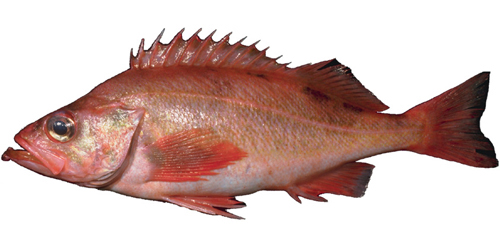
\includegraphics{Sebastes_alutus}~\\[0.5cm]
%\pdftooltip{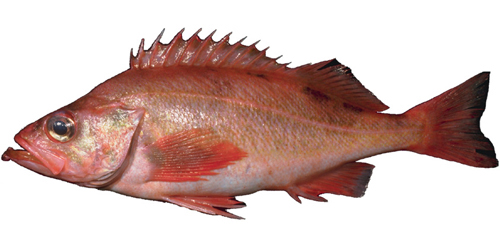
\includegraphics{Sebastes_alutus}}{This is a fish.}



Chantel R. Wetzel\textsuperscript{1}\\
Kelli Johnson\textsuperscript{2}\\
Lee Cronin-Fine\textsuperscript{3}\\

\vspace{.5cm}

\small
\textsuperscript{1}Northwest Fisheries Science Center, U.S. Department of Commerce, National Oceanic and Atmospheric Administration, National Marine Fisheries Service, 2725 Montlake Boulevard East, Seattle, Washington 98112\\

\vspace{.3cm}

\textsuperscript{2}Northwest Fisheries Science Center, U.S. Department of Commerce, National Oceanic and Atmospheric Administration, National Marine Fisheries Service, 2725 Montlake Boulevard East, Seattle, Washington 98112\\

\vspace{.3cm}

\textsuperscript{3}University of Washington, School of Aquatic and Fishery Sciences\\

\vspace{.3cm}

%\textsuperscript{4}Oregon Department of Fish and Wildlife, 2040 SE Marine Science Drive, Newport, OR 97365\\


\vspace{.5cm}

\vfill
DRAFT SAFE\\
Disclaimer: This information is distributed solely for the purpose of pre-dissemination
peer review under applicable information quality guidelines. It has not been formally
disseminated by NOAA Fisheries. It does not represent and should not be construed to
represent any agency determination or policy. 

\vspace{.3cm}
%Bottom of the page
%{\large \today}

\maketitle

\pagenumbering{roman}
\setcounter{page}{1}
\end{center}

{
\setcounter{tocdepth}{4}
\tableofcontents
}
\setlength{\parskip}{5mm plus1mm minus1mm} \pagebreak

\pagenumbering{arabic} \setcounter{page}{1}
\renewcommand{\thefigure}{\alph{figure}}
\renewcommand{\thetable}{\alph{table}}

\section*{Executive Summary}\label{executive-summary}
\addcontentsline{toc}{section}{Executive Summary}

\subsection*{Stock}\label{stock}
\addcontentsline{toc}{subsection}{Stock}

\hl{Include: species/area, including an evaluation of any potential biological basis 
for regional management.}

This assessment reports the status of the Pacific ocean perch
(\emph{Sebastes alutus}) resource in U.S. waters off the coast of the
California, Oregon, and Washington using data through 2017. Etc\ldots{}

\subsection*{Catches}\label{catches}
\addcontentsline{toc}{subsection}{Catches}

\hl{Include: trends and current levels-include table for last ten years and graph with 
long term data}

Catch figure(s) with fleets: (Figures
\ref{fig:Exec_catch1}-\ref{fig:Exec_catch3})\\
Catch table: (Table \ref{tab:Exec_catch})

\FloatBarrier

\begin{figure}
\centering
\includegraphics{Assessment_template_files/figure-latex/unnamed-chunk-2-1.pdf}
\caption{Pacific ocean perch landings in \ldots{}..
\label{fig:Exec_catch1}}
\end{figure}

\FloatBarrier

\begin{figure}
\centering
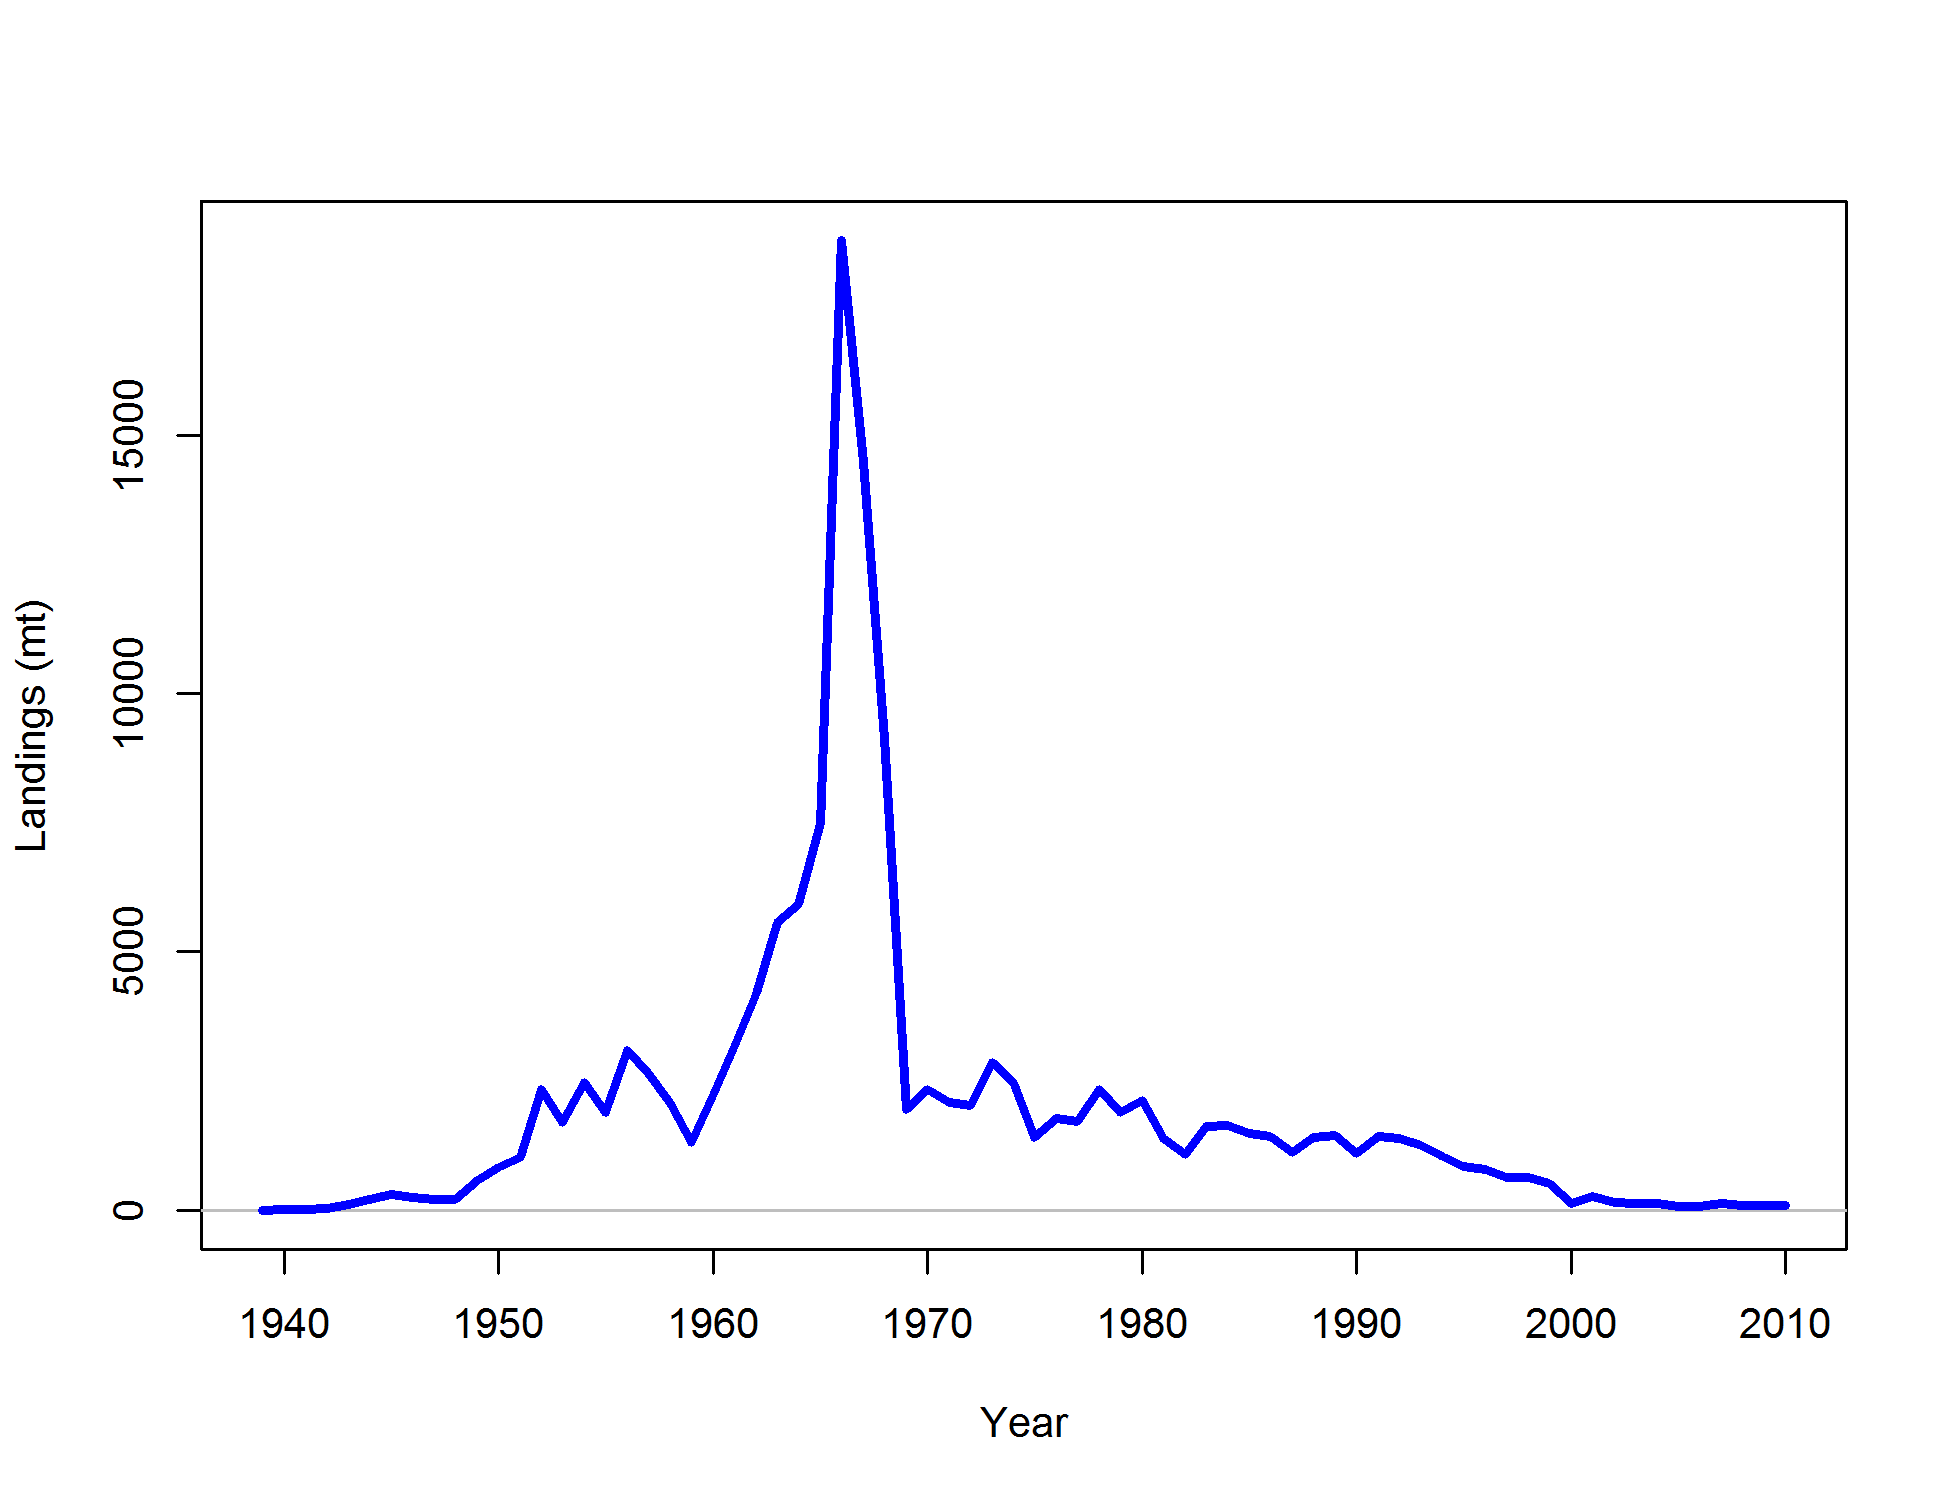
\includegraphics{r4ss/plots_mod1/catch1 landings.png}
\caption{Landings history of Pacific ocean perch in the Base model.
\label{fig:r4ss_catches}}
\end{figure}

\begin{table}[ht]
\centering
\caption{Recent Pacific ocean perch landings (mt) by 
                                            fleet.} 
\label{tab:Exec_catch}
\begin{tabular}{l>{\centering}p{0.7in}>{\centering}p{0.7in}>{\centering}p{0.7in}>{\centering}p{0.7in}>{\centering}p{0.7in}>{\centering}p{0.7in}}
  \hline
Year & California & Oregon & Washington & At-sea-hake & Survey & Total Catch \\ 
  \hline
\hline
\end{tabular}
\end{table}

\FloatBarrier

\newpage

\subsection*{Data and Assessment}\label{data-and-assessment}
\addcontentsline{toc}{subsection}{Data and Assessment}

\hl{Include: date of last assessment, type of assessment model, data available, new 
information, and information lacking.}

Pacific ocean perch was assessed\ldots{}. This assessment uses the
newest version of Stock Synthesis (3.30). The model begins in 1892, and
assumes the stock was at an unfished equilibrium that year.

\FloatBarrier

\subsection*{Stock Biomass}\label{stock-biomass}
\addcontentsline{toc}{subsection}{Stock Biomass}

\hl{Include: trends and current levels relative to virgin or historic levels, 
description of uncertainty-include table for last 10 years and graph with 
long term estimates.}

Spawning output Figure: Figure \ref{fig:Spawnbio_all}\\
Spawning output Table(s): Table \ref{tab:SpawningDeplete_mod1}\\
Relative depletion Figure: Figure \ref{fig:RelDeplete_all}

Example text (remove Models 2 and 3 if not needed - if using, remove the
\# in-line comments!!!)\\
The estimated relative depletion level (spawning output relative to
unfished spawning output) of the the base-case model in 2017 is 23\%
(\textasciitilde{}95\% asymptotic interval: \(\pm\) 23\%-23\%) (Figure
\ref{fig:RelDeplete_all}).

The estimated relative depletion level of model 2 in 2017 is
(\textasciitilde{}95\% asymptotic interval: \(\pm\) ) (Figure
\ref{fig:RelDeplete_all}).

The estimated relative depletion level of model 3 in 2017 is
(\textasciitilde{}95\% asymptotic interval: \(\pm\) ) (Figure
\ref{fig:RelDeplete_all}).

\FloatBarrier

\begin{table}[ht]
\centering
\caption{Recent trend in beginning of the 
                                      year spawning output and depletion for
                                      the Base model for Pacific ocean perch.} 
\label{tab:SpawningDeplete_mod1}
\begin{tabular}{l>{\centering}p{1.3in}>{\centering}p{1.2in}>{\centering}p{1in}>{\centering}p{1.2in}}
  \hline
Year & Spawning Output (billion eggs) & \~{} 95\% confidence interval & Estimated depletion & \~{} 95\% confidence interval \\ 
  \hline
2008 & 12648.00 & 12648 - 12648 & 0.19 & 0.188 - 0.188 \\ 
  2009 & 12994.00 & 12994 - 12994 & 0.19 & 0.193 - 0.193 \\ 
  2010 & 13132.00 & 13132 - 13132 & 0.20 & 0.195 - 0.195 \\ 
  2011 & 13211.00 & 13211 - 13211 & 0.20 & 0.196 - 0.196 \\ 
  2012 & 13347.00 & 13347 - 13347 & 0.20 & 0.198 - 0.198 \\ 
  2013 & 13684.00 & 13684 - 13684 & 0.20 & 0.203 - 0.203 \\ 
  2014 & 14133.00 & 14133 - 14133 & 0.21 & 0.210 - 0.210 \\ 
  2015 & 14644.00 & 14644 - 14644 & 0.22 & 0.218 - 0.218 \\ 
  2016 & 15081.00 & 15081 - 15081 & 0.22 & 0.224 - 0.224 \\ 
  2017 & 15448.00 & 15448 - 15448 & 0.23 & 0.230 - 0.230 \\ 
   \hline
\end{tabular}
\end{table}

\FloatBarrier

\begin{figure}
\centering
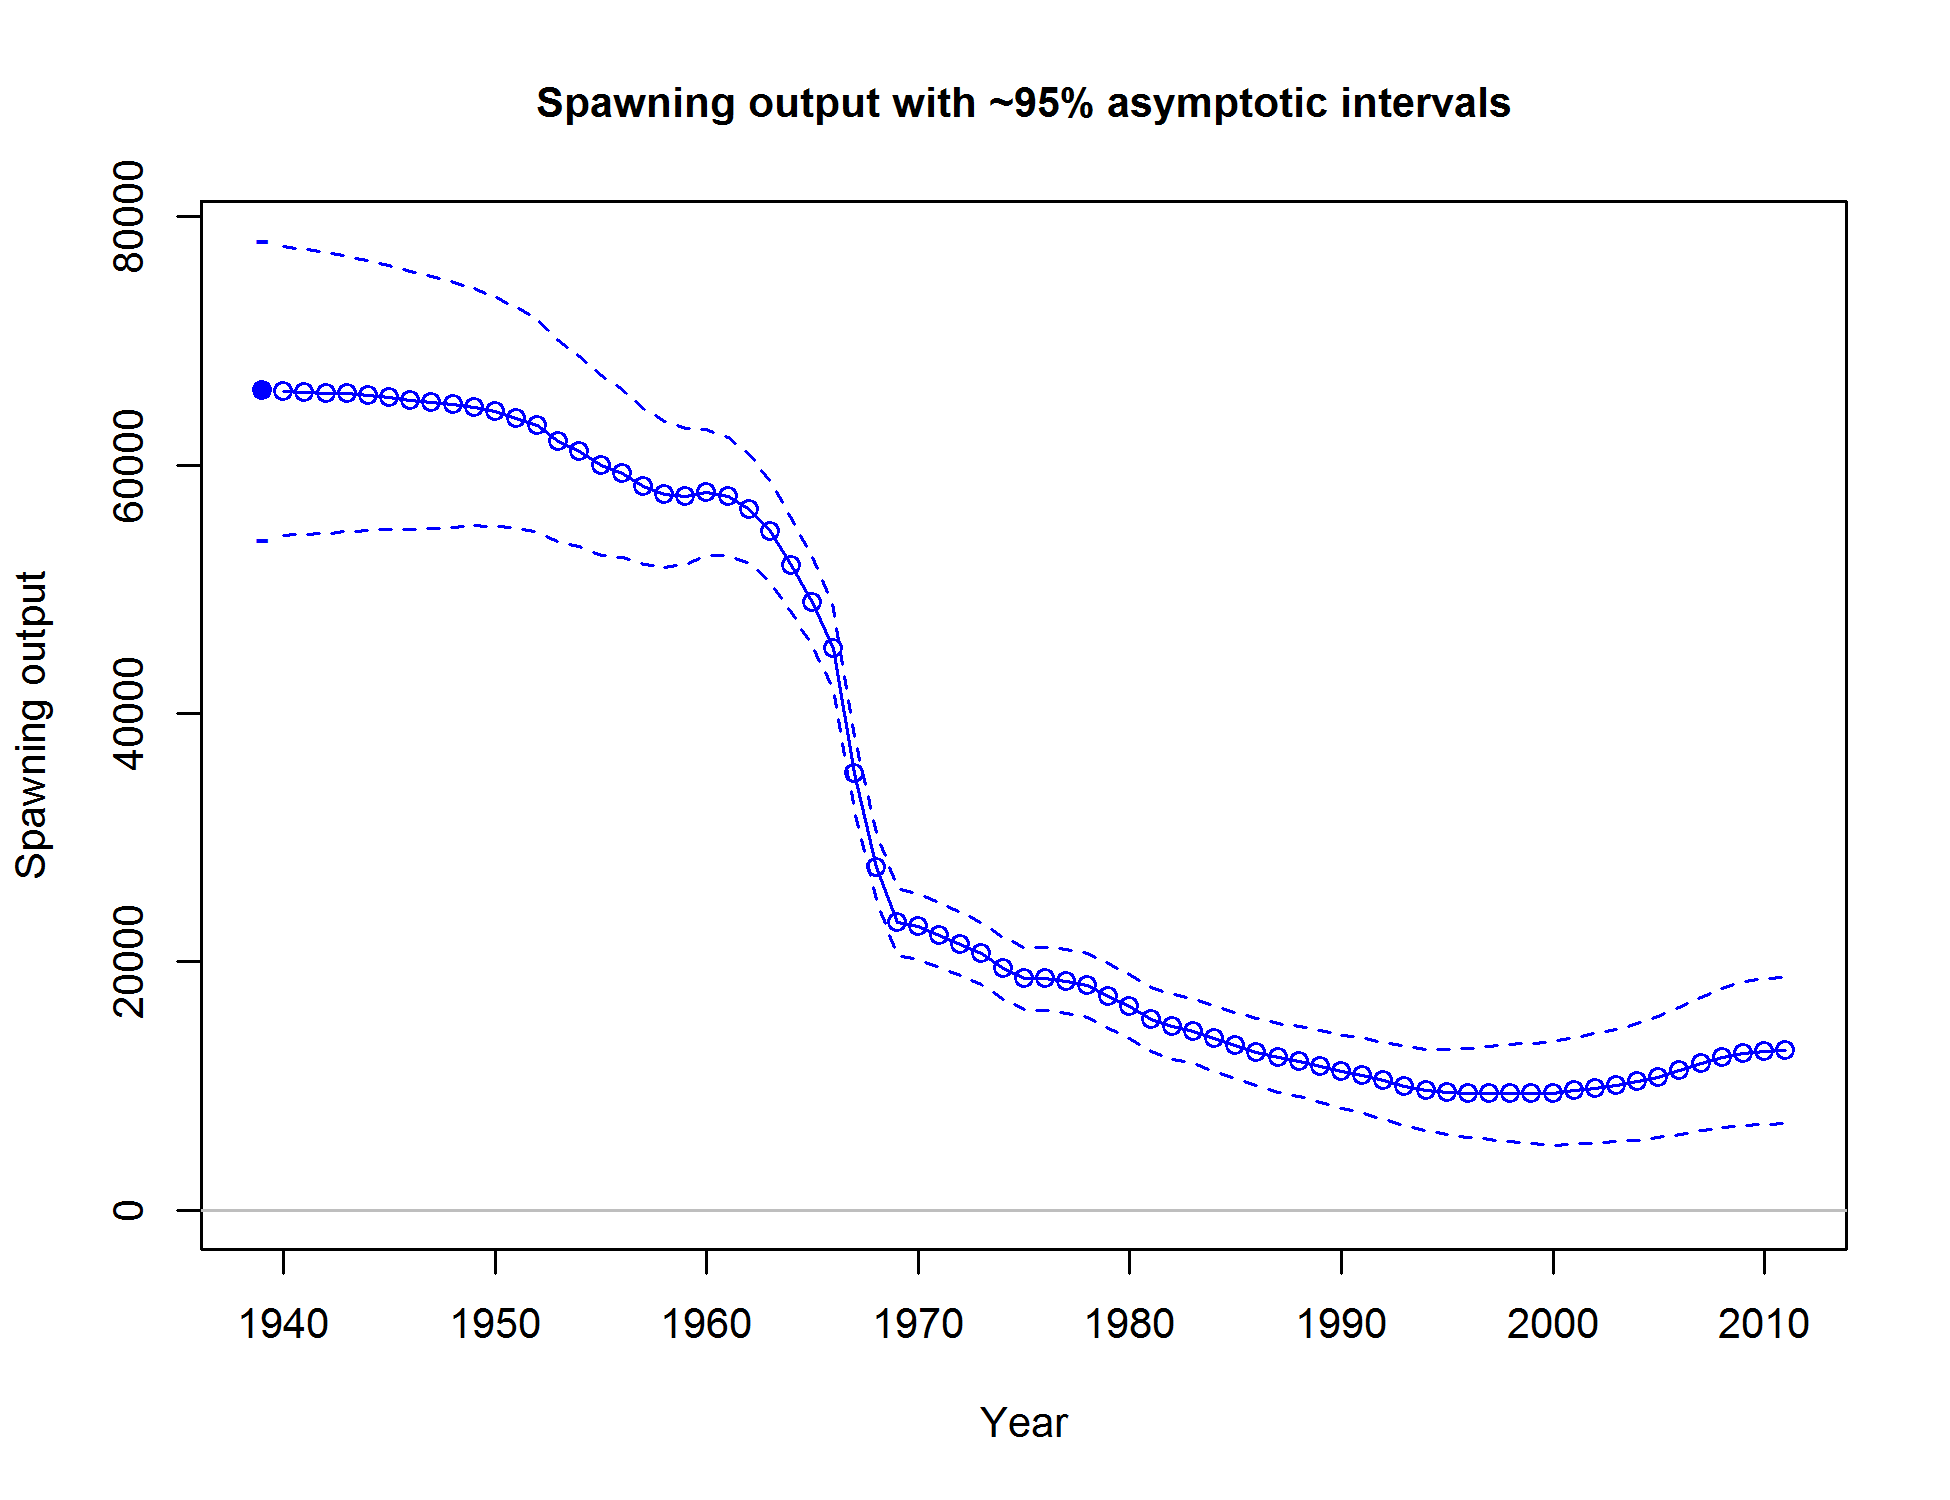
\includegraphics{r4ss/plots_mod1/ts7_Spawning_output_with_95_asymptotic_intervals_intervals.png}
\caption{Time series of spawning output trajectory (circles and line:
median; light broken lines: 95\% credibility intervals) for the base
case assessment model. \label{fig:Spawnbio_all}}
\end{figure}

\begin{figure}
\centering
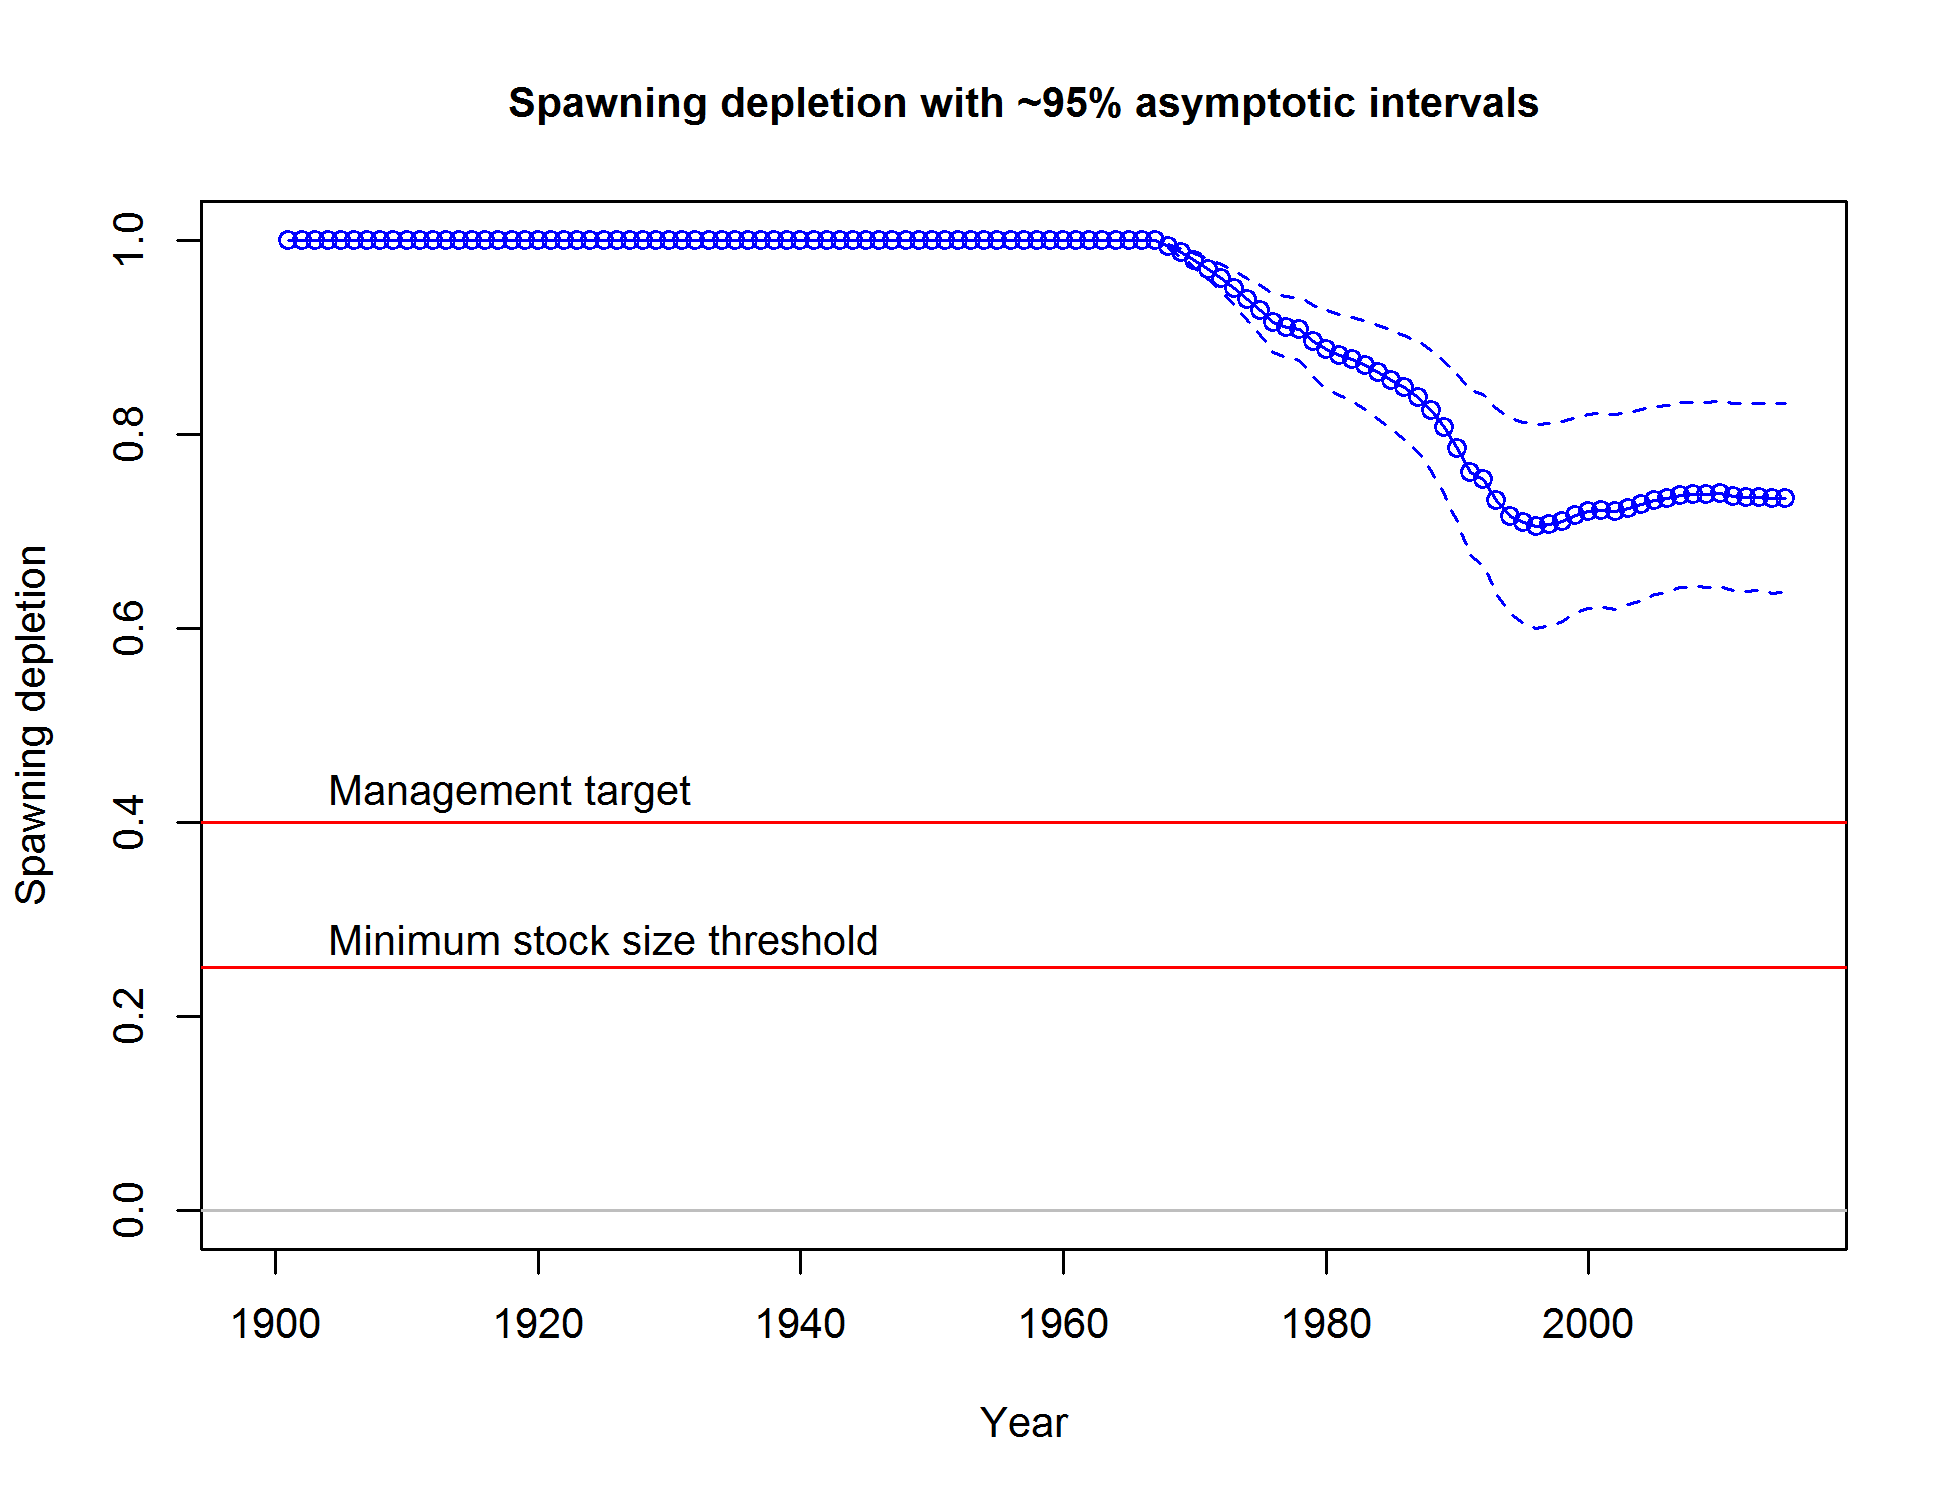
\includegraphics{r4ss/plots_mod1/ts9_Spawning_depletion_with_95_asymptotic_intervals_intervals.png}
\caption{Estimated relative depletion with approximate 95\% asymptotic
confidnce intervals (dashed lines) for the base case assessment model.
\label{fig:RelDeplete_all}}
\end{figure}

\FloatBarrier

\subsection*{Recruitment}\label{recruitment}
\addcontentsline{toc}{subsection}{Recruitment}

\hl{Include: trends and current levels relative to virgin or historic levels-include 
table for last 10 years and graph with long term estimates.}

Recruitment Figure: (Figure \ref{fig:Recruits_all})\\
Recruitment Tables: (Tables \ref{tab:Recruit_mod1},
\ref{tab:Recruit_mod2} and \ref{tab:Recruit_mod3})

\begin{table}[ht]
\centering
\caption{Recent recruitment for the Base model.} 
\label{tab:Recruit_mod1}
\begin{tabular}{>{\centering}p{.8in}>{\centering}p{1.6in}>{\centering}p{1.3in}}
  \hline
Year & Estimated Recruitment (1,000s) & \~{} 95\% confidence interval \\ 
  \hline
2008 & 10654.00 & 10654 - 10654 \\ 
  2009 & 2373.00 & 2373 - 2373 \\ 
  2010 & 3035.00 & 3035 - 3035 \\ 
  2011 & 3048.00 & 3048 - 3048 \\ 
  2012 & 3299.00 & 3299 - 3299 \\ 
  2013 & 3611.00 & 3611 - 3611 \\ 
  2014 & 3972.00 & 3972 - 3972 \\ 
  2015 & 4078.00 & 4078 - 4078 \\ 
  2016 & 4166.00 & 4166 - 4166 \\ 
  2017 & 4240.00 & 4240 - 4240 \\ 
   \hline
\end{tabular}
\end{table}

\FloatBarrier

\begin{figure}
\centering
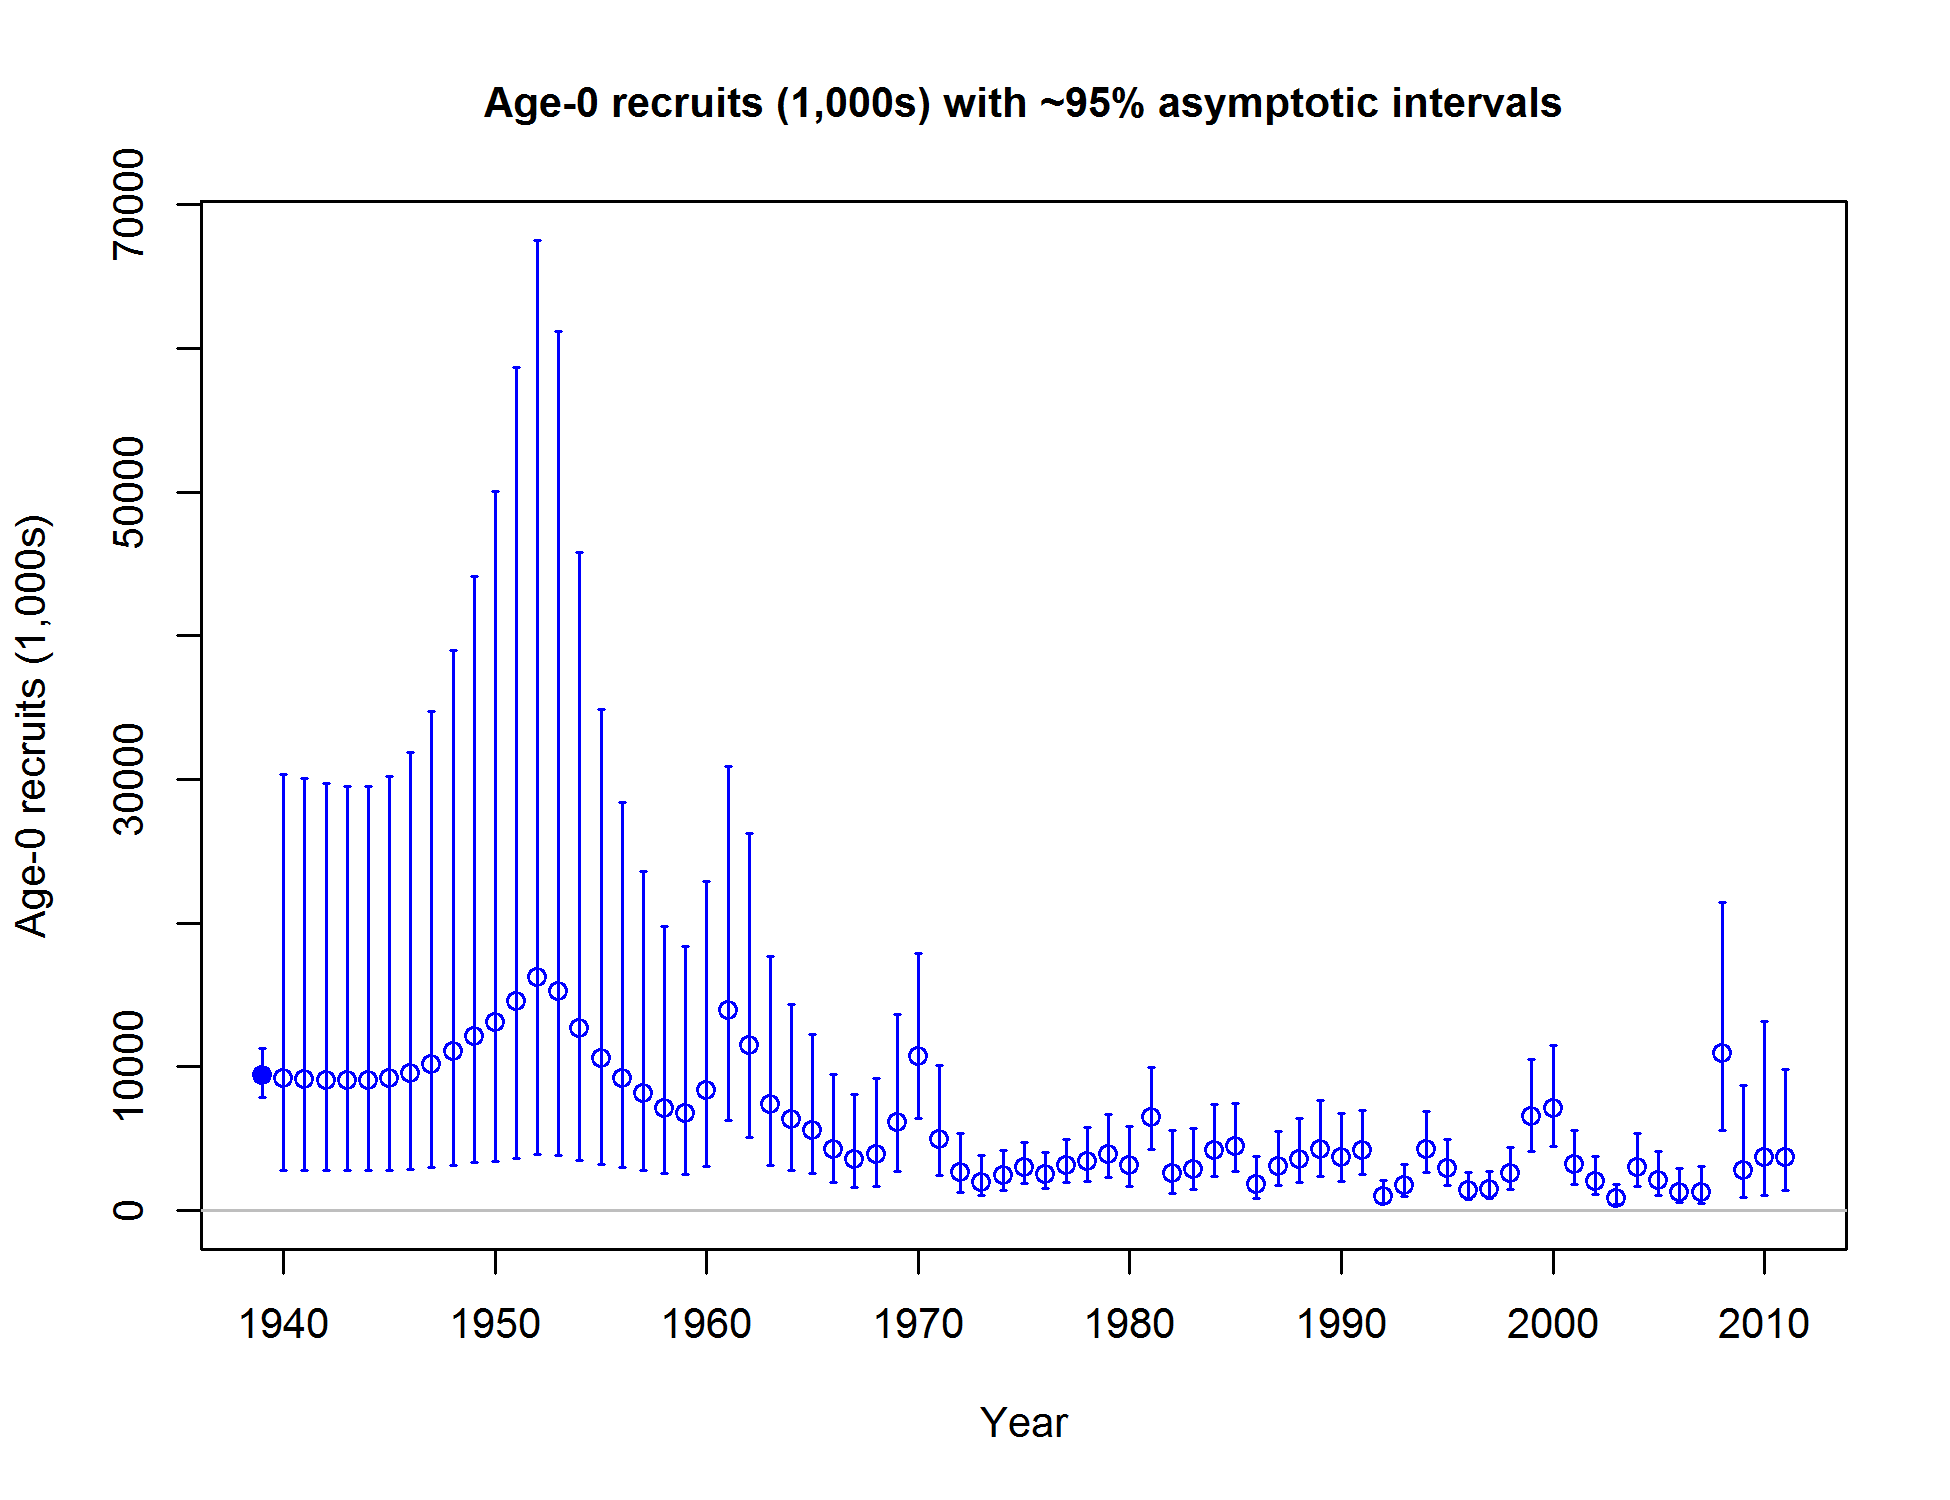
\includegraphics{r4ss/plots_mod1/ts11_Age-0_recruits_(1000s)_with_95_asymptotic_intervals.png}
\caption{Time series of estimated Pacific ocean perch recruitments for
the base-case model with 95\% confidence or credibility intervals.
\label{fig:Recruits_all}}
\end{figure}

\FloatBarrier

\subsection*{Exploitation status}\label{exploitation-status}
\addcontentsline{toc}{subsection}{Exploitation status}

\hl{Include: exploitation rates (i.e., total catch divided by exploitable biomass, or the annual SPR harvest rate) – include a table with the last 10 years of data and a graph showing the trend in fishing mortality relative to the target (y-axis) plotted against the trend in biomass relative to the target (x-axis).}

Exploitation Tables: Table \ref{tab:SPR_Exploit_mod1}, Table
\ref{tab:SPR_Exploit_mod2}, Table \ref{tab:SPR_Exploit_mod3}
Exploitation Figure: Figure \ref{fig:SPR_all}).

A summary of Pacific ocean perch exploitation histories for base model
is provided as Figure \ref{fig:Phase_all}.

\FloatBarrier

\begin{table}[ht]
\centering
\caption{Recent trend in spawning potential 
                                        ratio and exploitation for Pacific ocean perch in the Base model.  Fishing intensity is (1-SPR) 
                                        divided by 50\% (the SPR target) and exploitation 
                                        is F divided by F\textsubscript{SPR}.} 
\label{tab:SPR_Exploit_mod1}
\begin{tabular}{l>{\centering}p{1in}>{\centering}p{1.2in}>{\centering}p{1in}>{\centering}p{1.2in}}
  \hline
Year & Fishing intensity & \~{} 95\% confidence interval & Exploitation rate & \~{} 95\% confidence interval \\ 
  \hline
2007 & 0.296 & 0.296 - 0.296 & 0.006 & 0.006 - 0.006 \\ 
  2008 & 0.264 & 0.264 - 0.264 & 0.006 & 0.006 - 0.006 \\ 
  2009 & 0.352 & 0.352 - 0.352 & 0.008 & 0.008 - 0.008 \\ 
  2010 & 0.268 & 0.268 - 0.268 & 0.006 & 0.006 - 0.006 \\ 
  2011 & 0.169 & 0.169 - 0.169 & 0.003 & 0.003 - 0.003 \\ 
  2012 & 0.164 & 0.164 - 0.164 & 0.003 & 0.003 - 0.003 \\ 
  2013 & 0.158 & 0.158 - 0.158 & 0.003 & 0.003 - 0.003 \\ 
  2014 & 0.125 & 0.125 - 0.125 & 0.002 & 0.002 - 0.002 \\ 
  2015 & 0.160 & 0.160 - 0.160 & 0.003 & 0.003 - 0.003 \\ 
  2016 & 0.148 & 0.148 - 0.148 & 0.003 & 0.003 - 0.003 \\ 
   \hline
\end{tabular}
\end{table}

\FloatBarrier

\begin{figure}
\centering
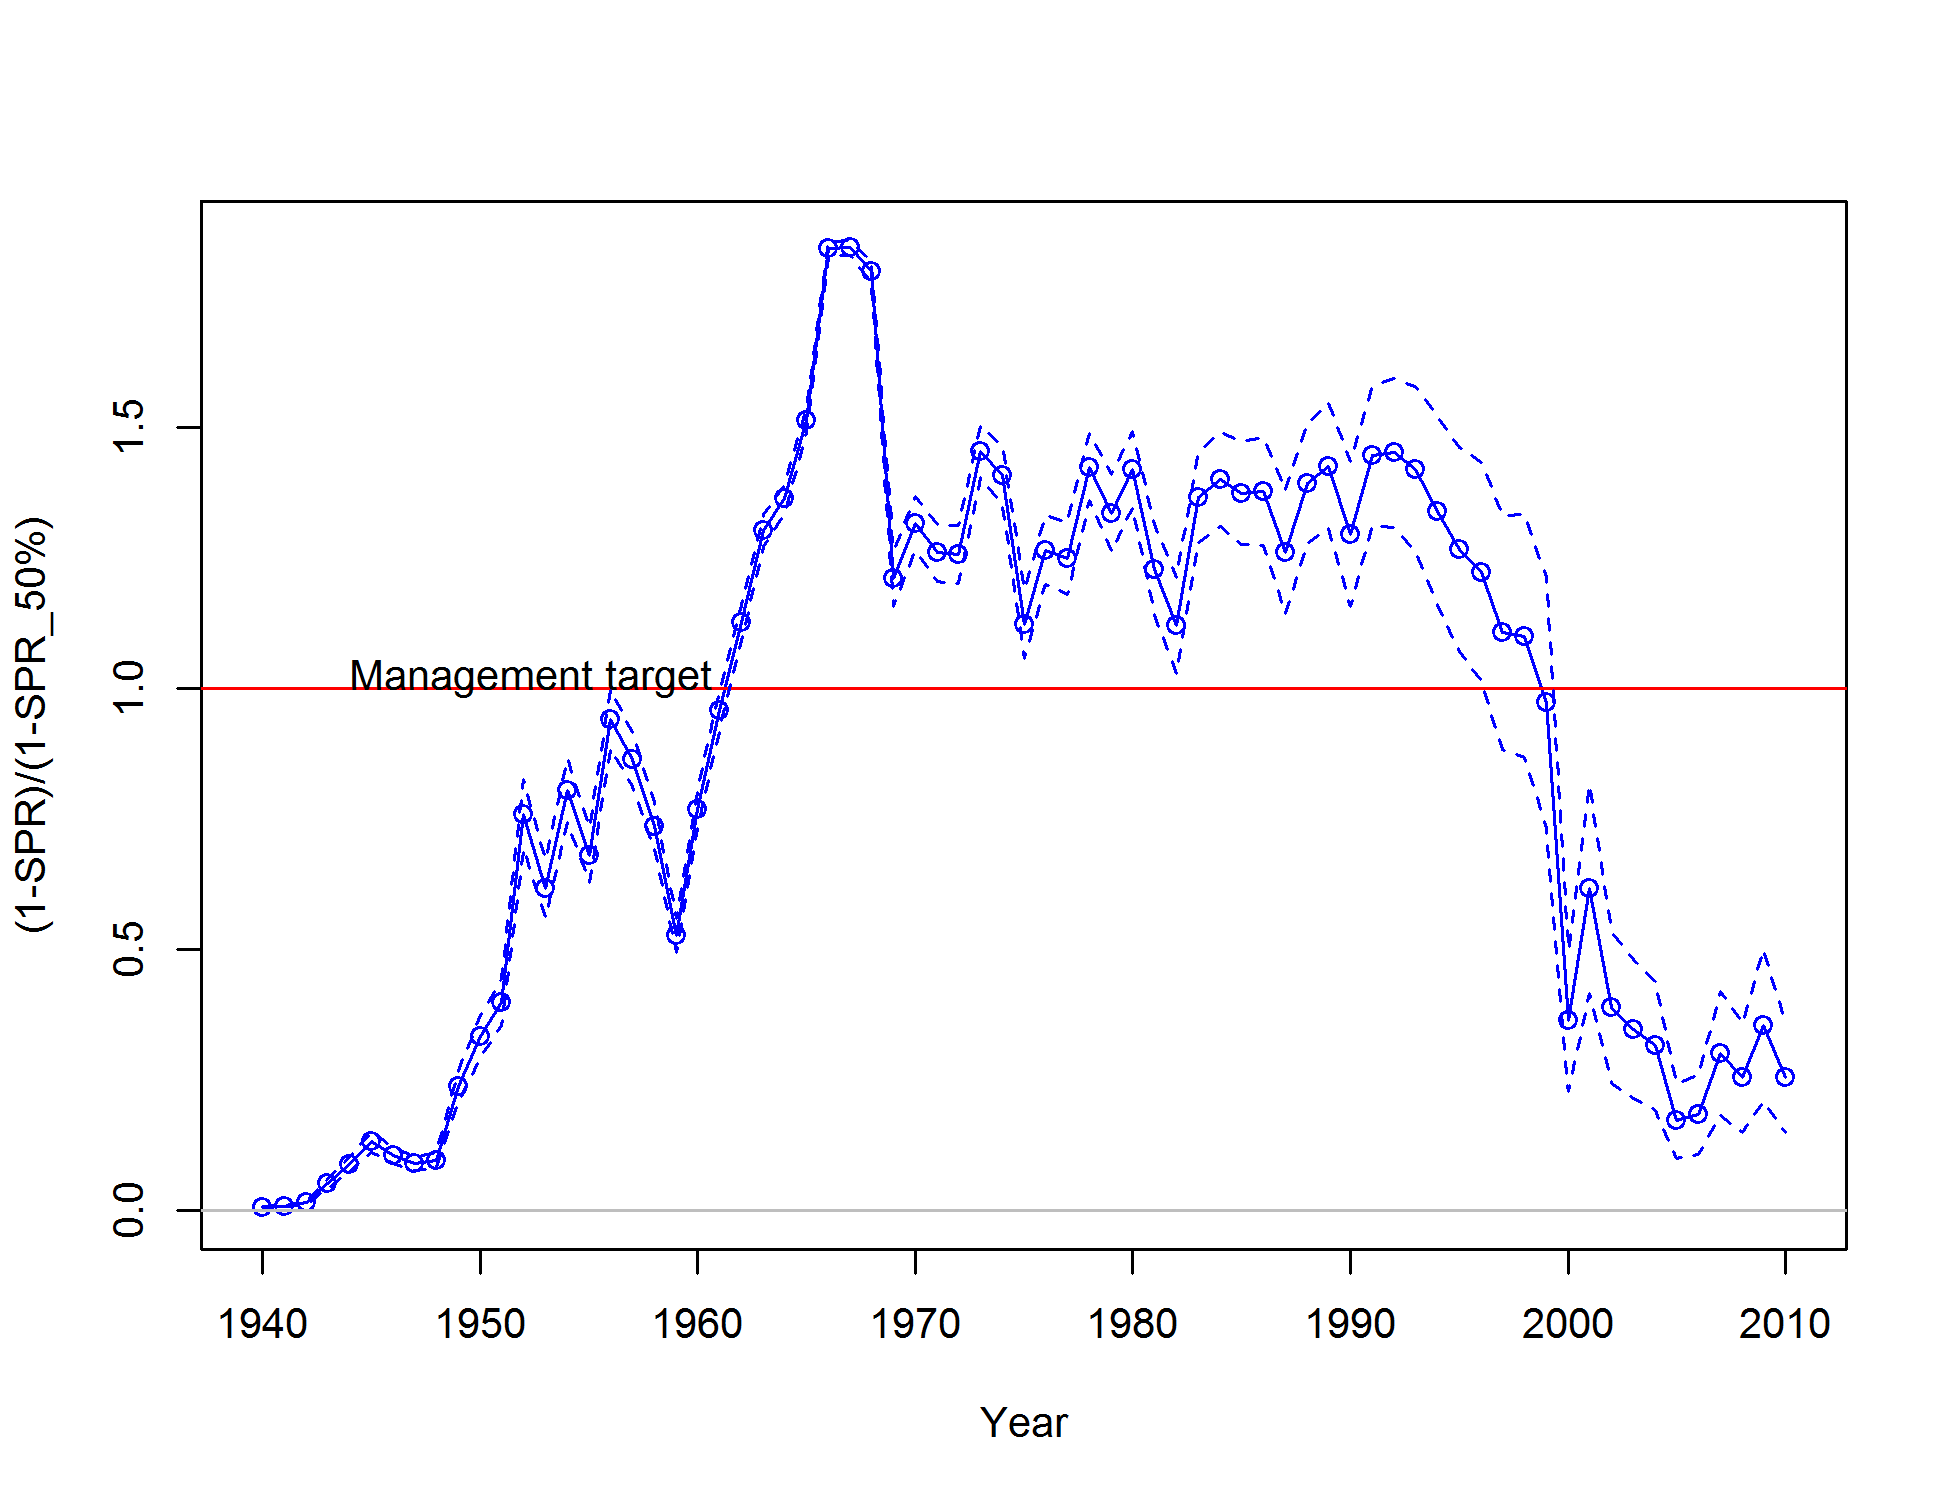
\includegraphics{r4ss/plots_mod1/SPR3_ratiointerval.png}
\caption{Estimated spawning potential ratio (SPR) for the base-case
model. One minus SPR is plotted so that higher exploitation rates occur
on the upper portion of the y-axis. The management target is plotted as
a red horizontal line and values above this reflect harvests in excess
of the overfishing proxy based on the SPR\textsubscript{50\%} harvest
rate. The last year in the time series is 2016. \label{fig:SPR_all}}
\end{figure}

\begin{figure}
\centering
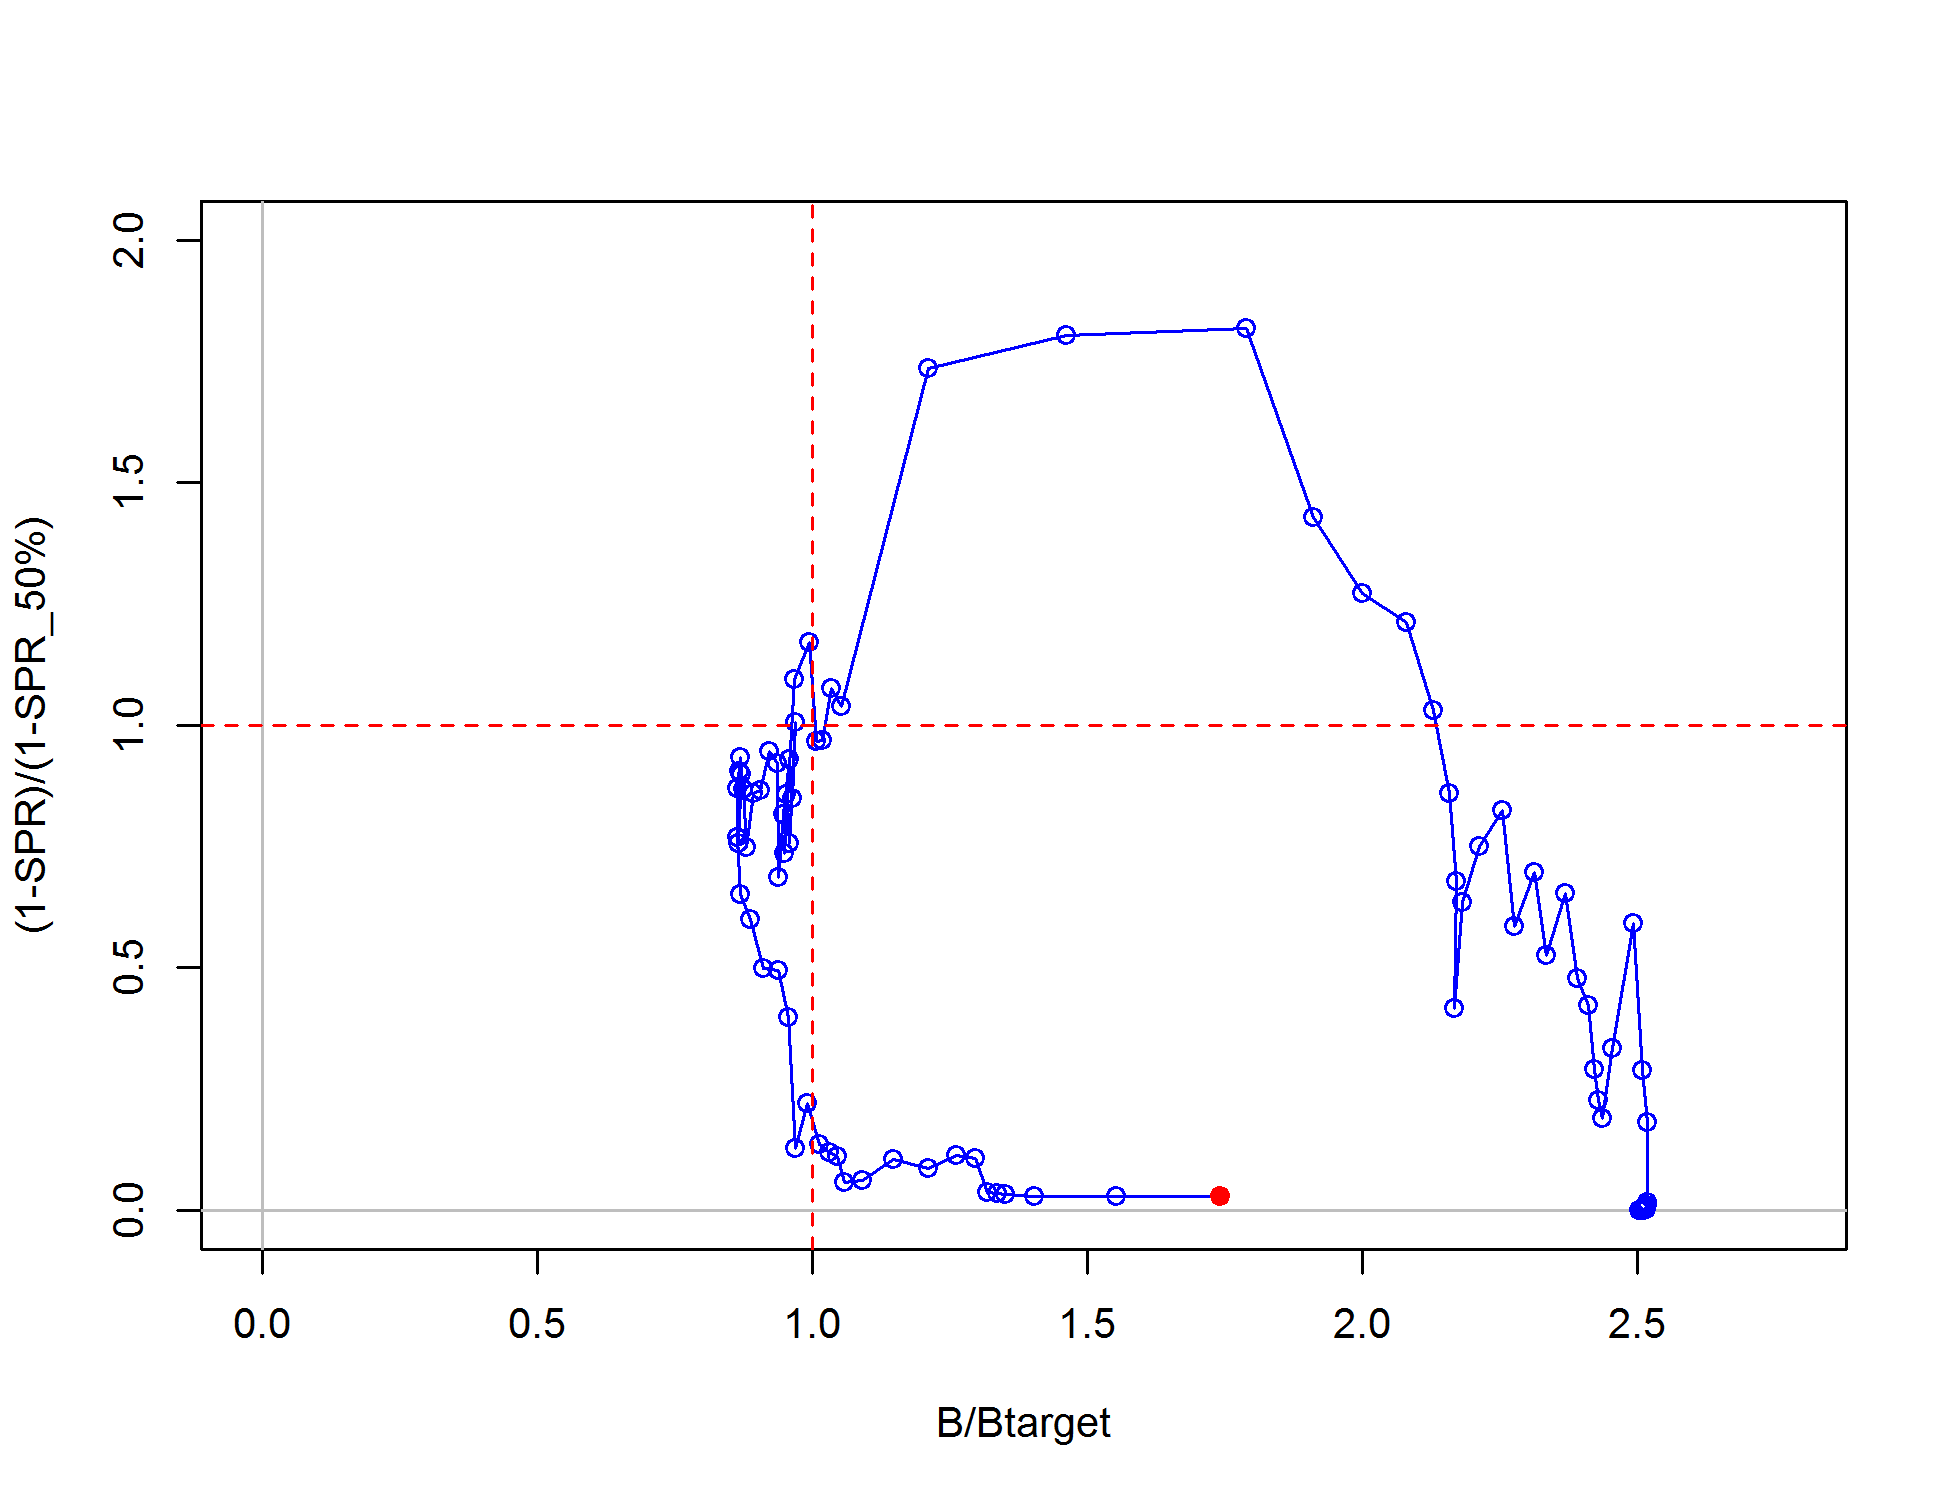
\includegraphics{r4ss/plots_mod1/SPR4_phase.png}
\caption{Phase plot of estimated relative (1-SPR) vs.~relative spawning
biomass for the base case model. The relative (1-SPR) is (1-SPR) divided
by 50\% (the SPR target). Relative depletion is the annual spawning
biomass divided by the unfished spawning biomass. \label{fig:Phase_all}}
\end{figure}

\FloatBarrier

\subsection*{Ecosystem Considerations}\label{ecosystem-considerations}
\addcontentsline{toc}{subsection}{Ecosystem Considerations}

In this assessment, ecosystem considerations were\ldots{}..

\subsection*{Reference Points}\label{reference-points}
\addcontentsline{toc}{subsection}{Reference Points}

\hl{Include:} management targets and definition of overfishing,
including the harvest rate that brings the stock to equilibrium at
\(B_{40\%}\) (the \(B_{MSY}\) proxy) and the equilibrium stock size that
results from fishing at the default harvest rate (the \(F_{MSY}\)
proxy). Include a summary table that compares estimated reference points
for SSB, SPR, Exploitation Rate and Yield based on SSBproxy for MSY,
SPRproxy for MSY, and estimated MSY values

\hl{Write intro paragraph....and remove text for Models 2 and 3 if not needed}

This stock assessment estimates that Pacific ocean perch in the Base
model are below the biomass target, but below the minimum stock size
threshold. \hl{Add sentence about spawning output trend.} The estimated
relative depletion level for \hl{Model 1} in 2017 is 23\%
(\textasciitilde{}95\% asymptotic interval: \(\pm\) 23\%-23\%,
corresponding to an unfished spawning output of 15448 billion eggs
(\textasciitilde{}95\% asymptotic interval: 15448.2-15448.2 billion
eggs) of spawning output in the base model (Table
\ref{tab:Ref_pts_mod1}). Unfished age 3+ biomass was estimated to be
123687 mt in the base case model. The target spawning output based on
the biomass target (\(SB_{40\%}\)) is 26914.1 billion eggs, which gives
a catch of 1083.8 mt. Equilibrium yield at the proxy \(F_{MSY}\) harvest
rate corresponding to \(SPR_{50\%}\) is 885 mt.

This stock assessment estimates that Pacific ocean perch in the are

the biomass target, but\\
the minimum stock size threshold.
\hl{Add sentence about spawning output trend.} The estimated relative
depletion level for \hl{Model 2} in 2017 is (\textasciitilde{}95\%
asymptotic interval: \(\pm\) ), corresponding to an unfished spawning
output of (\textasciitilde{}95\% asymptotic interval: ) of spawning
output in the base model (Table \ref{tab:Ref_pts_mod2}). Unfished age 3+
biomass was estimated to be\\
mt in the base case model. The target spawning output based on the
biomass target (\(SB_{40\%}\)) is , which gives a catch of mt.
Equilibrium yield at the proxy \(F_{MSY}\) harvest rate corresponding to
\(SPR_{50\%}\) is mt.

This stock assessment estimates that Pacific ocean perch in the are

the biomass target, but\\
the minimum stock size threshold.
\hl{Add sentence about spawning output trend.} The estimated relative
depletion level or \hl{Model 3} in 2017 is (\textasciitilde{}95\%
asymptotic interval: \(\pm\) ), corresponding to an unfished spawning
output of (\textasciitilde{}95\% asymptotic interval: ) of spawning
output in the base model (Table \ref{tab:Ref_pts_mod3}). Unfished age 3+
biomass was estimated to be mt in the base case model. The target
spawning output based on the biomass target (\(SB_{40\%}\)) is , which
gives a catch of mt. Equilibrium yield at the proxy \(F_{MSY}\) harvest
rate corresponding to \(SPR_{50\%}\) is mt.

\FloatBarrier

\begin{table}[ht]
\centering
\caption{Summary of reference 
                                      points and management quantities for the 
                                      base case Base model.} 
\label{tab:Ref_pts_mod1}
\begin{tabular}{>{\raggedright}p{4.1in}>{\centering}p{.65in}>{\centering}p{1.4in}}
  \hline
\textbf{Quantity} & \textbf{Estimate} & \textbf{\~95\%  Confidence Interval} \\ 
  \hline
Unfished spawning output (billion eggs) & 67285.2 & 67285.2 - 67285.2 \\ 
  Unfished age 3+ biomass (mt) & 123687 &  123687 -  123687 \\ 
  Unfished recruitment (R0, thousands) & 9574.5 &  9574.5 -  9574.5 \\ 
  Spawning output(2017 billion eggs) & 15448.2 & 15448.2 - 15448.2 \\ 
  Depletion (2017) & 0.23 &    0.23 -    0.23 \\ 
  \textbf{$\text{Reference points based on } \mathbf{SB_{40\%}}$} &  &  \\ 
  Proxy spawning output ($B_{40\%}$) & 26914.1 & 26914.1 - 26914.1 \\ 
  SPR resulting in $B_{40\%}$ ($SPR_{B40\%}$) & 0.625 &   0.625 -   0.625 \\ 
  Exploitation rate resulting in $B_{40\%}$ & 0.021 &   0.021 -   0.021 \\ 
  Yield with $SPR_{B40\%}$ at $B_{40\%}$ (mt) & 1083.8 &  1083.8 -  1083.8 \\ 
  \textbf{\textit{Reference points based on SPR proxy for MSY}} &  &  \\ 
  Spawning output & 13457 &   13457 -   13457 \\ 
  $SPR_{proxy}$ & 0.5 &  \\ 
  Exploitation rate corresponding to $SPR_{proxy}$ & 0.032 &   0.032 -   0.032 \\ 
  Yield with $SPR_{proxy}$ at $SB_{SPR}$ (mt) & 885 &     885 -     885 \\ 
  \textbf{\textit{Reference points based on estimated MSY values}} &  &  \\ 
  Spawning output at $MSY$ ($SB_{MSY}$) & 26279.6 & 26279.6 - 26279.6 \\ 
  $SPR_{MSY}$ & 0.619 &   0.619 -   0.619 \\ 
  Exploitation rate at $MSY$ & 0.021 &   0.021 -   0.021 \\ 
  $MSY$ (mt)  & 1084.2 &  1084.2 -  1084.2 \\ 
   \hline
\end{tabular}
\end{table}

\FloatBarrier

\subsection*{Management Performance}\label{management-performance}
\addcontentsline{toc}{subsection}{Management Performance}

\hl{Include: catches in comparison to OFL, ABC and OY/ACL values for the most 
recent 10 years (when available), overfishing levels, actual catch and discard. 
Include OFL(encountered), OFL(retained) and OFL(dead) if different due to discard 
and discard mortality.}

Management performance table: Table \ref{tab:mnmgt_perform}

\begin{table}[ht]
\centering
\caption{Recent trend in total catch and commercial 
                              landings (mt) relative to the management guidelines. 
                              Estimated total catch reflect the commercial landings 
                              plus the model estimated discarded biomass.} 
\label{tab:mnmgt_perform}
\scalebox{0.9}{
\begin{tabular}{>{\raggedleft}p{1in}>{\centering}p{1in}>{\centering}p{1in}>{\centering}p{1in}>{\centering}p{1in}}
  \hline
Year & OFL (mt; ABC prior to 2011) & ABC (mt) & ACL (mt; OY prior to 2011) & Estimated total catch (mt) \\ 
  \hline
\textbf{2007} & - & - & - & - \\ 
  \textbf{2008} & - & - & - & - \\ 
  \textbf{2009} & - & - & - & - \\ 
  \textbf{2010} & - & - & - & - \\ 
  \textbf{2011} & - & - & - & - \\ 
  \textbf{2012} & - & - & - & - \\ 
  \textbf{2013} & - & - & - & - \\ 
  \textbf{2014} & - & - & - & - \\ 
  \textbf{2015} & - & - & - & - \\ 
  \textbf{2016} & - & - & - & - \\ 
   \hline
\end{tabular}
}
\end{table}

\subsection*{Unresolved Problems And Major
Uncertainties}\label{unresolved-problems-and-major-uncertainties}
\addcontentsline{toc}{subsection}{Unresolved Problems And Major
Uncertainties}

TBD after STAR panel

\FloatBarrier

\subsection*{Decision Table(s) (groundfish
only)}\label{decision-tables-groundfish-only}
\addcontentsline{toc}{subsection}{Decision Table(s) (groundfish only)}

\hl{Include: projected yields (OFL, ABC and ACL), spawning biomass, and stock 
depletion levels for each year. Not required in draft assessments undergoing review.}

OFL projection table: Table \ref{tab:OFL_projection}

Decision table(s) Table \ref{tab:Decision_table_mod1}, Table
\ref{tab:Decision_table_mod2}, Table \ref{tab:Decision_table_mod3}

\begin{verbatim}
Yield curve: Figure \ref{fig:Yield_all}
\end{verbatim}

\begin{table}[ht]
\centering
\caption{Projections of potential OFL (mt) and the ACL (mt) using the base model forecast.} 
\label{tab:OFL_projection}
\begin{tabular}{lrr}
  \hline
Year & OFL & ACL \\ 
  \hline
2017 & 989.34 &  \\ 
   \hline
\end{tabular}
\end{table}\begin{table}[ht]
\centering
\caption{Summary of 10-year 
                                             projections beginning in 2019 
                                             for alternate states of nature based on 
                                             an axis of uncertainty for the Base model.  Columns range over low, mid, and high
                                             states of nature, and rows range over different 
                                             assumptions of catch levels. An entry of "--" 
                                             indicates that the stock is driven to very low 
                                             abundance under the particular scenario.} 
\label{tab:Decision_table_mod1}
\scalebox{0.85}{
\begin{tabular}{l|cc|>{\centering}p{.7in}c|>{\centering}p{.7in}c|>{\centering}p{.7in}c}
   \multicolumn{3}{c}{}  &  \multicolumn{2}{c}{} 
                               & \multicolumn{2}{c}{\textbf{States of nature}} 
                               & \multicolumn{2}{c}{} \\
  \multicolumn{3}{c}{}  &  \multicolumn{2}{c}{Low M 0.05} 
                               & \multicolumn{2}{c}{Base M 0.07} 
                               &  \multicolumn{2}{c}{High M 0.09} \\
 \hline
 & Year & Catch & Spawning Output & Depletion & Spawning Output & Depletion & Spawning Output & Depletion \\ 
  \hline
 & 2019 & - & - & - & - & - & - & - \\ 
   & 2020 & - & - & - & - & - & - & - \\ 
   & 2021 & - & - & - & - & - & - & - \\ 
  40-10 Rule,  & 2022 & - & - & - & - & - & - & - \\ 
  Low M & 2023 & - & - & - & - & - & - & - \\ 
   & 2024 & - & - & - & - & - & - & - \\ 
   & 2025 & - & - & - & - & - & - & - \\ 
   & 2026 & - & - & - & - & - & - & - \\ 
   & 2027 & - & - & - & - & - & - & - \\ 
   & 2028 & - & - & - & - & - & - & - \\ 
   \hline
 & 2019 & - & - & - & - & - & - & - \\ 
   & 2020 & - & - & - & - & - & - & - \\ 
   & 2021 & - & - & - & - & - & - & - \\ 
  40-10 Rule & 2022 & - & - & - & - & - & - & - \\ 
   & 2023 & - & - & - & - & - & - & - \\ 
   & 2024 & - & - & - & - & - & - & - \\ 
   & 2025 & - & - & - & - & - & - & - \\ 
   & 2026 & - & - & - & - & - & - & - \\ 
   & 2027 & - & - & - & - & - & - & - \\ 
   & 2028 & - & - & - & - & - & - & - \\ 
   \hline
 & 2019 & - & - & - & - & - & - & - \\ 
   & 2020 & - & - & - & - & - & - & - \\ 
   & 2021 & - & - & - & - & - & - & - \\ 
  40-10 Rule, & 2022 & - & - & - & - & - & - & - \\ 
  High M & 2023 & - & - & - & - & - & - & - \\ 
   & 2024 & - & - & - & - & - & - & - \\ 
   & 2025 & - & - & - & - & - & - & - \\ 
   & 2026 & - & - & - & - & - & - & - \\ 
   & 2027 & - & - & - & - & - & - & - \\ 
   & 2028 & - & - & - & - & - & - & - \\ 
   \hline
 & 2019 & - & - & - & - & - & - & - \\ 
   & 2020 & - & - & - & - & - & - & - \\ 
   & 2021 & - & - & - & - & - & - & - \\ 
  Average & 2022 & - & - & - & - & - & - & - \\ 
  Catch & 2023 & - & - & - & - & - & - & - \\ 
   & 2024 & - & - & - & - & - & - & - \\ 
   & 2025 & - & - & - & - & - & - & - \\ 
   & 2026 & - & - & - & - & - & - & - \\ 
   & 2027 & - & - & - & - & - & - & - \\ 
   & 2028 & - & - & - & - & - & - & - \\ 
   \hline
\end{tabular}
}
\end{table}

\begin{sidewaystable}[ht]
\centering
\caption{Base case results summary.} 
\label{tab:base_summary}
\scalebox{0.6}{
\begin{tabular}{r>{\centering}p{1.1in}>{\centering}p{1.1in}>{\centering}p{1.1in}>{\centering}p{1.1in}>{\centering}p{1.1in}>{\centering}p{1.1in}>{\centering}p{1.1in}>{\centering}p{1.1in}>{\centering}p{1.1in}>{\centering}p{1.1in}}
  \hline
Quantity & 2009 & 2010 & 2011 & 2012 & 2013 & 2014 & 2015 & 2016 & 2017 & 2018 \\ 
  \hline
Landings (mt) &  &  &  &  &  &  &  &  &  &  \\ 
  Total Est. Catch (mt) &  &  &  &  &  &  &  &  &  &  \\ 
  OFL (mt) &  &  &  &  &  &  &  &  &  &  \\ 
  ACL (mt) &  &  &  &  &  &  &  &  &  &  \\ 
   \hline
(1-$SPR$)(1-$SPR_{50\%}$) & 0.26 & 0.35 & 0.27 & 0.17 & 0.16 & 0.16 & 0.13 & 0.16 & 0.15 &  \\ 
   \hline
Exploitation rate & 0.01 & 0.01 & 0.01 & 0.00 & 0.00 & 0.00 & 0.00 & 0.00 & 0.00 &  \\ 
  Age 3+ biomass (mt) & 25305.3 & 25578.9 & 25651.6 & 26743.3 & 27334.8 & 27963.1 & 28570.0 & 29189.2 & 29794.3 & 30433.8 \\ 
   \hline
Spawning Output & 12648 & 12994 & 13132 & 13211 & 13347 & 13684 & 14133 & 14644 & 15081 & 15448 \\ 
  ~95\% CI & 12648 - 12648 & 12994 - 12994 & 13132 - 13132 & 13211 - 13211 & 13347 - 13347 & 13684 - 13684 & 14133 - 14133 & 14644 - 14644 & 15081 - 15081 & 15448 - 15448 \\ 
   \hline
Depletion & 0.188 & 0.193 & 0.195 & 0.196 & 0.198 & 0.203 & 0.210 & 0.218 & 0.224 & 0.230 \\ 
  ~95\% CI & 0.188 - 0.188 & 0.193 - 0.193 & 0.195 - 0.195 & 0.196 - 0.196 & 0.198 - 0.198 & 0.203 - 0.203 & 0.210 - 0.210 & 0.218 - 0.218 & 0.224 - 0.224 & 0.230 - 0.230 \\ 
   \hline
Recruits & 10654 &  2373 &  3035 &  3048 &  3299 &  3611 &  3972 &  4078 &  4166 &  4240 \\ 
  ~95\% CI & 10654 - 10654 & 2373 - 2373 & 3035 - 3035 & 3048 - 3048 & 3299 - 3299 & 3611 - 3611 & 3972 - 3972 & 4078 - 4078 & 4166 - 4166 & 4240 - 4240 \\ 
   \hline
\end{tabular}
}
\end{sidewaystable}

\begin{figure}
\centering
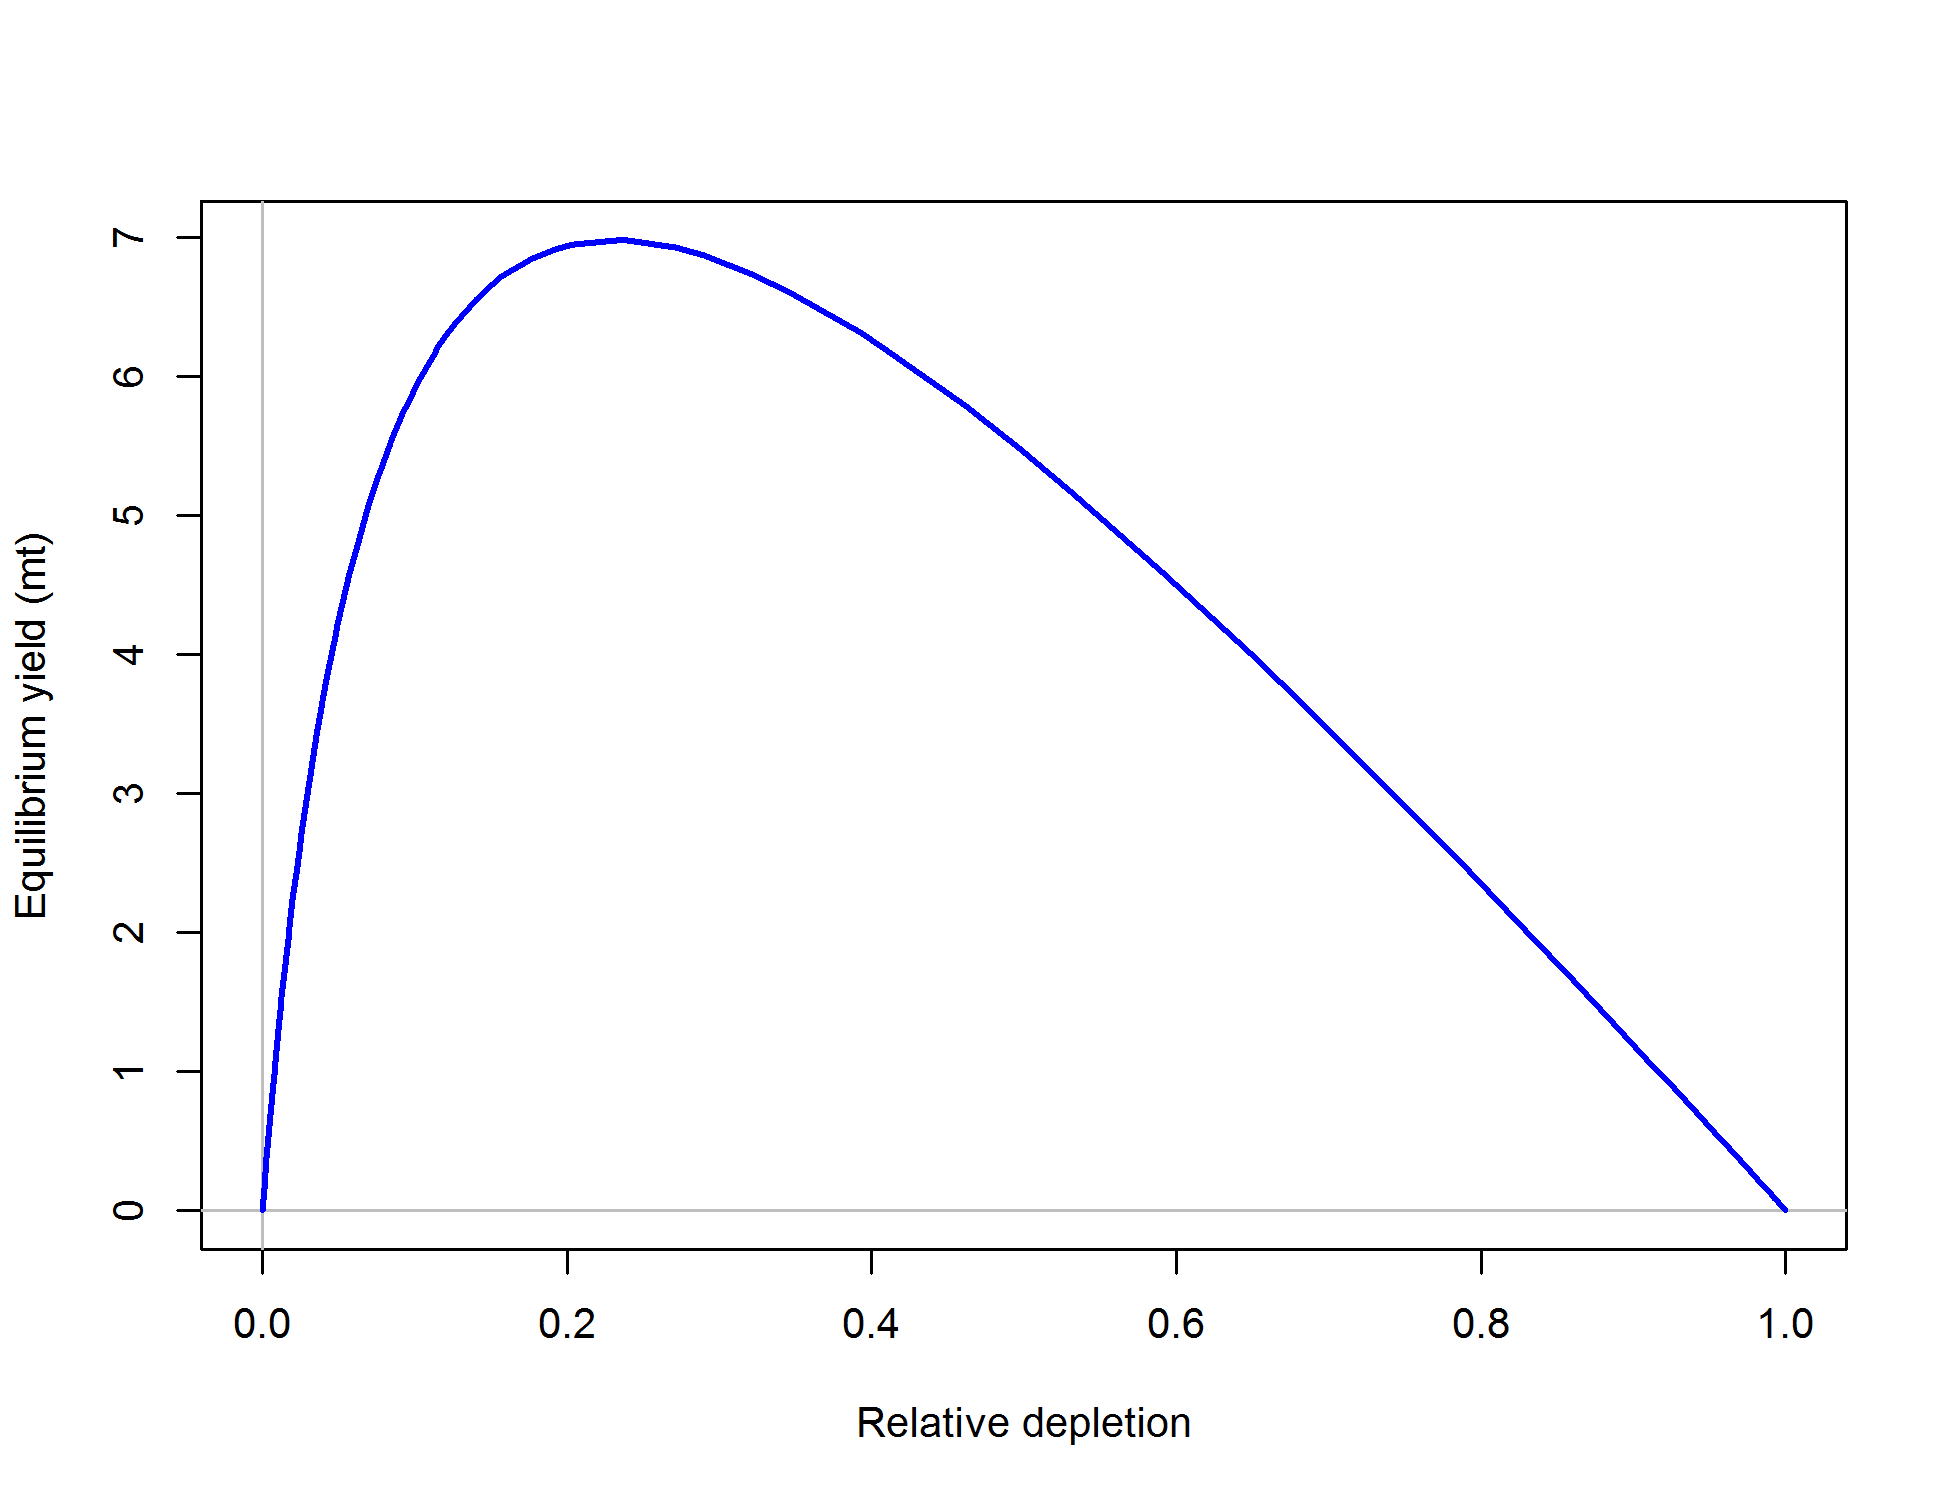
\includegraphics{r4ss/plots_mod1/yield1_yield_curve.png}
\caption{Equilibrium yield curve for the base case model. Values are
based on the 2016 fishery selectivity and with steepness fixed
at\ldots{} \label{fig:Yield_all}}
\end{figure}

\FloatBarrier

\newpage

\subsection*{Research And Data Needs}\label{research-and-data-needs}
\addcontentsline{toc}{subsection}{Research And Data Needs}

\hl{Include: identify information gaps that seriously impede the stock assessment.}

We recommend the following research be conducted before the next
assessment:

\begin{enumerate}

\item List item No. 1 in the list

\item List item No. 2 in the list, etc.

\end{enumerate}

\subsection*{Rebuilding Projections}\label{rebuilding-projections}
\addcontentsline{toc}{subsection}{Rebuilding Projections}

\hl{Include: reference to the principal results from rebuilding analysis if the 
stock is overfished. This section should be included in the Final/SAFE version 
assessment document but is not required for draft assessments undergoing review. 
See Rebuilding Analysis terms of reference for detailed information on 
rebuilding analysis requirements.}

\FloatBarrier

\newpage

\renewcommand{\thefigure}{\arabic{figure}}
\renewcommand{\thetable}{\arabic{table}}

\setcounter{figure}{0} \setcounter{table}{0}

\section{Introduction}\label{introduction}

\subsection{Basic Information}\label{basic-information}

Pacific ocean perch (\emph{Sebastes alutus}) are most abundant in the
Gulf of Alaska, and have been observed off of Japan, in the Bering Sea,
and south to Baja California, although they are sparse south of Oregon
and rare in southern California. While genetic studies have found three
populations of Pacific ocean perch off of British Columbia (Seeb and
Gunderson \protect\hyperlink{ref-seeb_genetic_1988}{1988}, Withler et
al. \protect\hyperlink{ref-withler_co-existing_2001}{2001}) with,
notably, a separate stock off of Vancouver Island, no significant
genetic differences have been found in the range covered by this
assessment. Pacific ocean perch show dimorphic growth, with females
reaching a slightly large size than males. Males and females are equally
abundant on rearing grounds at age 1.5.

The Pacific ocean perch population has been modeled as a single stock
off of the U.S. West Coast (essentially northern California to the
Canadian border, since Pacific ocean perch are seen extremely rarely in
central and southern California). Good recruitments show up in
size-composition data throughout all portions of this area, which
supports the single stock hypothesis. This assessment includes landings
and catch data for Pacific ocean perch from the states of Washington,
Oregon and California, along with records from foreign fisheries, the
at-sea hake fleet, and surveys.

Prior to 1966, the Pacific ocean perch resource off of the northern
portion of the U.S. West Coast was harvested almost entirely by Canadian
and United States vessels. Harvest was negligible prior to 1940, reached
\hl{1,000} mt in 1951, \hl{3,000} mt in 1961 and exceeded \hl{7,000} mt
in 1965. Catches increased dramatically after 1965, with the
introduction of large distant-water fishing fleets from the Soviet Union
and Japan. Both nations employed large factory stern trawlers as their
primary method for harvesting Pacific ocean perch. Peak removals by all
foreign nations combined are estimated at over \hl{15,000} mt in 1966
and remained over \hl{12,000} mt in 1967. These numbers are based upon a
re-analysis of the foreign catch data (Rogers
\protect\hyperlink{ref-rogers_species_2003}{2003}), which focused on
deriving a more realistic species composition for catches previously
identified only as Pacific ocean perch. Catches declined rapidly
following these peak years, and Pacific ocean perch stocks were
considered to be severely depleted throughout the Oregon-Vancouver
Island region by 1969 (Gunderson
\protect\hyperlink{ref-gunderson_population_1977}{1977}, Gunderson et
al. \protect\hyperlink{ref-gunderson_status_1977}{1977}). Landed harvest
averaged \hl{1,500} mt over the period 1977-94. Landings have continued
to decline since 1994, primarily due to more restrictive management.

Prior to 1977, Pacific ocean perch in the northeast Pacific were managed
by the Canadian Government in its waters and by the individual states in
waters off of the United States. With implementation of the Magnuson
Fishery Conservation and Management Act (MFCMA) in 1977, U.S.
territorial waters were extended to 200 miles from shore, and primary
responsibility for management of the groundfish stocks off Washington,
Oregon and California shifted from the states to the Pacific Fishery
Management Council (PFMC) and the National Marine Fisheries Service
(NMFS). At that time, however, a Fishery Management Plan (FMP) for the
west coast groundfish stocks had not yet been approved. In the interim,
the state agencies worked with the PFMC to address conservation issues.
In 1981, the PFMC adopted a management strategy to rebuild the depleted
Pacific ocean perch stocks to levels that would produce Maximum
Sustainable Yield (MSY) within 20 years. On the basis of cohort analysis
(Gunderson \protect\hyperlink{ref-gunderson_results_1978}{1978}), the
PFMC set Acceptable Biological Catch (ABC) levels at 600 mt for the US
portion of the Vancouver INPFC area and 950 mt for the Columbia INPFC
area. To implement this strategy, the states of Oregon and Washington
each established landing limits for Pacific ocean perch. Trawl trip
limits of various forms remained in effect through 2010 (\hl{Table 1}).

Age estimates for Pacific ocean perch prior to the 1980s were made via
surface ageing of otoliths, which misses the very tight annuli at the
edge of the otolith once the fish reaches near maximum size. Ages are
biased by around age 10-12, and maximum age was estimated to be in the
20s, which lead to an overestimate of the natural mortality rate and the
productivity of the stock. Using break and burn methods, Pacific ocean
perch have been aged to over 100 years, and we now know that the
underlying assumptions of the early models were overly optimistic about
productivity. Research surveys have been used to provide
fishery-independent information about the abundance, distribution, and
biological characteristics of Pacific ocean perch. A coast-wide survey
of the rockfish resource was conducted in 1977 (Gunderson and Sample
\protect\hyperlink{ref-gunderson_distribution_1980}{1980}) and was
repeated every three years through 2004. The National Marine Fisheries
Service (NMFS) coordinated a cooperative research survey of the Pacific
ocean perch stocks off Washington and Oregon with the Washington
Department of Fisheries (WDFW) and the Oregon Department of Fish and
Wildlife (ODFW) in March-May 1979 (Wilkins and Golden
\protect\hyperlink{ref-wilkins_condition_1983}{1983}). This survey was
repeated in 1985. Two slope surveys have been conducted on the west
coast in recent years, one using the research vessel Miller Freeman,
which ended in 2001, and another ongoing cooperative survey using
commercial fishing vessels which began in 1998 as a DTS (Dover sole,
thornyhead and sablefish) survey, was expanded to other groundfish in
1999. In 2003, this survey was expanded spatially to include the shelf.
This last survey, conducted by the NWFSC, continues to cover depths from
30-700 fathoms (55-1280 meters) on an annual basis.

\subsection{Map}\label{map}

A map showing the scope of the assessment and depicting boundaries for
fisheries or data collection strata is provided in Figure
\ref{fig:boundary_map}.

\subsection{Life History}\label{life-history}

\hl{Include: Important features of life history that affect management (e.g., migration, 
sexual dimorphism, bathymetric demography).}

\subsection{Ecosystem Considerations}\label{ecosystem-considerations-1}

\hl{Include: Ecosystem considerations (e.g., ecosystem role and trophic relationships of 
the species, habitat requirements/preferences, relevant data on ecosystem processes 
that may affect stock or parameters used in the stock assessment, and/or cross-FMP 
interactions with other fisheries). This section should note if environmental 
correlations or food web interactions were incorporated into the assessment model. 
The length and depth of this section would depend on availability of data and reports 
from the IEA, expertise of the STAT, and whether ecosystem factors are informational 
to contribute quantitative information to the assessment.}

\subsection{Fishery Information}\label{fishery-information}

\hl{Include: Important features of current fishery and relevant history of fishery.}

\subsection{Summary of Management
History}\label{summary-of-management-history}

\hl{Include: Summary of management history (e.g., changes in mesh sizes, trip 
limits, or other management actions that may have significantly altered selection, 
catch rates, or discards).}

\subsection{Management Performance}\label{management-performance-1}

\hl{Include: Management performance, including a table or tables comparing 
Overfishing Limit (OFL), Annual Catch Limit (ACL), Harvest Guideline (HG) 
[CPS only], landings, and catch (i.e., landings plus discard) for each area and year.}

Management performance table: (Table \ref{tab:mnmgt_perform})\\
A summary of these values as well as other base case summary results can
be found in Table \ref{tab:base_summary}.

\subsection{Fisheries off Canada, Alaska, and/or
Mexico}\label{fisheries-off-canada-alaska-andor-mexico}

Include if necessary.

\section{Assessment}\label{assessment}

\subsection{Data}\label{data}

Data used in the Pacific ocean perch assessment are summarized in Figure
\ref{fig:data_plot}.\\
A description of each data source is below.

\subsubsection{Commercial Fishery
Landings}\label{commercial-fishery-landings}

\textbf{Washington}

Historical commercial fishery landigns of Pacific ocean perch from
Washington for the years 1918-1980 were obtained from Theresa Tsou
(WDFW) and Phillip Weyland (WDFW). This assessment is the first Pacific
ocean perch assessment to include a state provide historical catch
reconstruction and hence, the historical catches for Washington vary
markedly from those used in the 2011 assessment. Recent landings
(1981-2016) were obtained from PacFIN (Pacific Fisheries Information
Network (PacFIN) retrieval dated \hl{March 3, 2015}, Pacific States
Marine Fisheries Commission, Portland, Oregon; www.psmfc.org).

\textbf{Oregon}

Historical commercial fishery landings of Pacific ocean perch from
Oregon for the years 1892-1986 were obtained from Alison Dauble (ODFW).
A description of the methods can be found in (Karnowski et al.
\protect\hyperlink{ref-karnowski_historical_2014}{2014}). Recent
landings (1987-2016) were obtained from PacFIN (Pacific Fisheries
Information Network (PacFIN) retrieval dated \hl{March 3, 2015}, Pacific
States Marine Fisheries Commission, Portland, Oregon; www.psmfc.org).

\textbf{California}

Historical commercial fishery landings of Pacific ocean perch were
obtained from the online database of the California Cooperative
Groundfish Survey, also known as CALCOM (128.114.3.187) for the years
1916-1980. A description of the methods can be found in (Ralston et al.
\protect\hyperlink{ref-ralston_documentation_2010}{2010}). Recent
landings (1981-2016) were obtained from PacFIN (Pacific Fisheries
Information Network (PacFIN) retrieval dated \hl{March 3, 2015}, Pacific
States Marine Fisheries Commission, Portland, Oregon; www.psmfc.org).

\textbf{At-sea fishery}

Catches of Pacific ocean perch are monitored aboard the vessel by
observers in the At-Sea hake Observer program (ASHOP) and were available
for the years of 1975-2016. Observers use a spatial sample design, based
on weight, to randomly choose a portion of the haul to sample for
species composition. For the last decade, this is typically 30-50\% of
the total weight. The total weight of the sample is determined by all
catch passing over a flow scale. All species other than hake are removed
and weighed, by species, on a motion compensated flatbed scale.
Observers record the weights of all non-hake species. Non-hake species
total weights are expanded in the database by using the proportion of
the haul sampled to the total weight of the haul. The catches of
non-hake species in unsampled hauls is determined using bycatch rates
determined from sampled hauls. Since 2001, more than 97\% of the hauls
have been observed and sampled.

\textbf{Foreign}

From the 1960s through the early 1970s, foreign trawling enterprises
harvested considerable amounts of rockfish off Washington and Oregon,
and along with the domestic trawling fleet, landed large quantities of
`r spp'. Foreign catches of individual species were estimated by Rogers
(\protect\hyperlink{ref-rogers_species_2003}{2003}) and attributed to
INPFC areas for the years of 1966-1976 for `r spp'. The foreign catches
were combined across areas for a coastwide removal total.

\textbf{Discards}

\subsubsection{Abundance Indices}\label{abundance-indices}

\textbf{Sub-heading 1}

\textbf{Sub-heading 2}

\subsubsection{Fishery-Independent Data: possible
sources}\label{fishery-independent-data-possible-sources}

\textbf{Northwest Fisheries Science Center (NWFSC) shelf-slope survey}

The NWFSC shelf-slope survey is based on a random-grid design; covering
the coastal waters from a depth of 55 m to 1,280 m (Bradburn et al.
\protect\hyperlink{ref-bradburn_2003_2011}{2011}). This design uses four
chartered industry vessels in most years, assigned to a roughly equal
number of randomly selected grid cells. The survey, which has been
conducted from late-May to early-October each year, is divided into two
2-vessel passes of the coast, which are executed from north to south.
This design therefore incorporates both vessel-to-vessel differences in
catchability as well as variance associated with selecting a relatively
small number (\textasciitilde{}700) of cells from a very large
population of possible cells (greater than 11,000) distributed from the
Mexican to the Canadian border.

\textbf{Northwest Fisheries Science Center (NWFSC) slope survey}

The NWFSC slope survey covered waters throughout the summer from 183 m
to 1280 m north of \(34^\circ 30^\prime\) S, which is near Point
Conception. The survey strata used to expand the biomass data for this
assessment are shown in \hl{Table 5}.

\textbf{Alaska Fisheries Science Center (AFSC) slope survey}

The AFSC slope survey operated during autumn (October-November) aboard
the R/V Miller Freeman. Partial survey coverage of the U.S. west coast
occurred during 1988-96 and complete coverage (north of
\(34^\circ 30^\prime\) S) during 1997, 1999, 2000, and 2001. Only the
four years of consistent and complete surveys plus 1996, which surveyed
north of \(43^\circ\) N latitude to the U.S.-Canada border, were used in
this assessment. The number of tows ranged from
\hl{8 in 2001 to 26 in 1996 (Table 7)}. The numbers of tows with length
data for `r spp' are also shown in \hl{Table 7}.
\hl{Because a large number of positive tows occurred in 1996}, it was
decided to include that year, which surveyed from \(43^\circ\) N
latitude to the U.S.-Canada border. Therefore, only tows from
\(43^\circ\) N latitude to the U.S.-Canada border were used.

\textbf{Triennial Bottom Trawl Survey}

The triennial survey was first conducted by the AFSC in 1977 and spanned
the timeframe from 1977-2004. The survey's design and sampling methods
are most recently described in (Weinberg et al.
\protect\hyperlink{ref-weinberg_estimation_2002}{2002}). Its basic
design was a series of equally-spaced transects from which searches for
tows in a specific depth range were initiated \hl{(Figure 5)}. The
survey design has changed slightly over the period of time
\hl{(Table 4, Figure 3)}. In general, all of the surveys were conducted
in the mid-summer through early fall: the 1977 survey was conducted from
early July through late September; the surveys from 1980 through 1989
ran from mid-July to late September; the 1992 survey spanned from
mid-July through early October; the 1995 survey was conducted from early
June to late August; the 1998 survey ran from early June through early
August; and the 2001 and 2004 surveys were conducted in May-July
\hl{(Figure 4)}.

Haul depths ranged from 91-457 m during the 1977 survey with no hauls
shallower than 91 m. The surveys in 1980, 1983, and 1986 covered the
West Coast south to \(36.8^\circ\) N latitude and a depth range of
55-366 meters. The surveys in 1989 and 1992 covered the same depth range
but extended the southern range to \(34.5^\circ\) N (near Point
Conception). From 1995 through 2004, the surveys covered the depth range
55-500 meters and surveyed south to \(34.5^\circ\) N. In the final year
of the triennial series (2004), the NWFSC's Fishery Resource and
Monitoring division (FRAM) conducted the survey and followed very
similar protocols as the AFSC.

Given the different depths surveyed during 1977, the data from that year
were not included in this assessment. Water hauls (Zimmermann et al.
\protect\hyperlink{ref-zimmermann_influence_2003}{2003}) and tows
located in Canadian waters were also excluded from the analysis of this
survey. The survey was analyzed as an early series (1980-1992) and a
late series (1995-2004), as has been done in other West Coast rockfish
assessments.

\textbf{Pacific ocean perch Survey}

\textbf{Pikitch Study}

The Pikitch study was conducted between 1985 and 1987 (Pikitch et al.
\protect\hyperlink{ref-pikitch_evaluation_1988}{1988}). The northern and
southern boundaries of the study were \(48^\circ 42^\prime\) N latitude
and \(42^\circ 60^\prime\) N. latitude respectively, which is primarily
within the Columbia INPFC area (Pikitch et al.
\protect\hyperlink{ref-pikitch_evaluation_1988}{1988} , Rogers and
Pikitch \protect\hyperlink{ref-rogers_numerical_1992}{1992}).
Participation in the study was voluntary and included vessels using
bottom, midwater, and shrimp trawl gears.\\
Observers of normal fishing operations on commercial vessels collected
the data, estimated the total weight of the catch by tow and recorded
the weight of species retained and discarded in the sample.

\subsubsection{Biological Parameters and
Data}\label{biological-parameters-and-data}

\textbf{Length And Age Compositions}

Include: Sample size information for length and age composition data by
area, year, gear, market category, etc., including both the number of
trips and fish sampled.

Length compositions were provided from the following sources, by region,
with brief descriptions below:

\emph{Model 1}

\begin{itemize}[noitemsep,nolistsep,topsep=0pt]
  \item Source No. 1 (\emph{ex. research, commerical dead fish, live fish, etc},\\     
        date range (ex. 2010-2011)
  \item Source No. 2 (\emph{ex. research, commerical dead fish, live fish, etc},\\      
        date range (ex. 2010-2011) 
  \item etc...      
  \item Begin sublist if desired 
    \begin{itemize}[noitemsep,nolistsep]
      \item Sublist source No. 1     
      \item Sublist source No. 2        
      \item etc...     
    \end{itemize}
  \item Back to main list, next Source     
  \item Last Source     
\end{itemize}

Can duplicate this list if you have more than one assessment model

Possible sources of age and length data:

\emph{Recreational: Washington (WDFW)}

\emph{Recreational: California MRFSS And CRFS Length Composition Data}
Individual fish lengths recorded by MRFSS (1980-2003) and CRFS
(2004-2011) samplers were downloaded from the RecFIN website
(www.recfin.org). CRFS data from 2012-2014 were obtained directly from
CDFW.

\emph{Recreational: Oregon Recreational Boat Survey (ORBS)} Biological
data from the ORBS program were provided by ODFW. The ORBS is a dockside
sampling program for the both the recreational CPFV and private modes.
Length composition samples from north of Florence for the CPFV and
private fleets were provided from 1980-2014. Samples from south of
Florence spanned 1984-2014

\emph{Recreational: Miller and Gotshall ({\textbf{???}})}\\
The Northern California Marine Sport Fish Survey conducted an assessment
survey with goals that included estimation of annual fishing effort by
all recreational fishing modes, catch by weight, CPUE, and collection of
data to analyze length compositions

\emph{Commercial: PacFIN (Oregon and California)}

\emph{Research: NMFS Groundfish Ecology Survey}

From 2001-2005, the SWFSC Fisheries Ecology Division conducted longline
surveys aboard a chartered commercial longline vessel at various
stations between Monterey and Davenport, CA (\(36^\circ\) N. latitude to
\(37.5^\circ\) N. latitude) (pers. comm. Don Pearson, SWFSC). Longline
gear was set in various depths from 10 meters to 700 meters, parallel to
the depth contour. Each longline set consisted of 3-5 skates, each with
about 250 2/0 circle hooks baited with squid.\\
In nearshore habitats, the gear soaked for roughly 30 minutes.

\emph{Research: California Collaborative Fisheries Research Program
(CCFRP)}

\emph{Research: NWFSC shelf-slope survey}

\emph{Research: NWFSC slope survey}

\emph{Research: Abrams Thesis}

\vspace{.5cm} \textbf{Age Structures}

Age structure data were available from the following sources:

\emph{Model Region 1}

\begin{itemize}[noitemsep,nolistsep,topsep=0pt]
  \item Source No. 1 (\emph{ex. research, commericla dead fish, live fish, etc},\\ 
        date range (ex. 2010-2011)
  \item Source No. 2 (\emph{ex. research, commericla dead fish, live fish, etc},\\
        date range (ex. 2010-2011) 
  \item etc...      
  \item Begin sublist if desired 
    \begin{itemize}[noitemsep,nolistsep]
      \item Sublist source No. 1     
      \item Sublist source No. 2        
      \item etc...     
    \end{itemize}
  \item Back to main list, next Source     
  \item Last Source     
\end{itemize}

Can duplicate this list if you have more than one assessment model

Length-at-age was initially estimated external to the population
dynamics models using the von Bertalanffy growth curve ({\textbf{???}}),
\(L_i = L_{\infty}e^{(-k[t-t_0])}\), where \(L_i\) is the length (cm) at
age \(i\), \(t\) is age in years, \(k\) is rate of increase in growth,
\(t_0\) is the intercept, and \(L_{\infty}\) is the asymptotic length.

\vspace{.5cm} \textbf{Aging Precision And Bias}

\vspace{.5cm} \textbf{Weight-Length}

The weight-length relationship is based on the standard power function:
\(W = \alpha(L^\beta)\) where \(W\) is individual weight (kg), \(L\) is
length (cm), and \(\alpha\) and \(\beta\) are coefficients used as
constants.

\vspace{.5cm} \textbf{Maturity And Fecundity}

\vspace{.5cm} \textbf{Natural Mortality}

Natural mortality for wild fish populations is extremely difficult to
estimate.

\vspace{.5cm} \textbf{Sex ratios}

\subsubsection{Environmental Or Ecosystem Data Included In The
Assessment}\label{environmental-or-ecosystem-data-included-in-the-assessment}

\subsection{History Of Modeling Approaches Used For This
Stock}\label{history-of-modeling-approaches-used-for-this-stock}

\subsubsection{Previous Assessments}\label{previous-assessments}

\subsubsection{Previous Assessment
Recommendations}\label{previous-assessment-recommendations}

Include: Response to STAR panel recommendations from the most recent
previous assessment.

\begin{description}[style=unboxed]

  \item[Recommendation 1: blah blah blah.] \hfill \\

   STAT response: blah blah blah....

\item[Recommendation 2: blah blah blah.] \hfill \\

  STAT response: blah blah blah....

\item[Recommendation 3: blah blah blah., etc.] \hfill \\

  STAT response: Continue recommendations as needed


\end{description}

\subsection{Model Description}\label{model-description}

\subsubsection{Transition To The Current Stock
Assessment}\label{transition-to-the-current-stock-assessment}

Include: Complete description of any new modeling approaches

Below, we describe the most important changes made since the last full
assessment and explain rationale for each change.:

\begin{enumerate}
\def\labelenumi{\arabic{enumi}.}
\item
  Change No. 1. \emph{Rationale}: blah blah blah.
\item
  Change No. 2. \emph{Rationale}: blah blah blah.
\item
  Change No. 3. \emph{Rationale}: Continue list as needed.
\end{enumerate}

\subsubsection{Definition of Fleets and
Areas}\label{definition-of-fleets-and-areas}

We generated data sources for each of the models. Fleets by model
include:

\textbf{Model Region 1 or remove this line if only one model}

\emph{Commercial}: The commercial fleets include\ldots{}

\emph{Recreational}: The recreational fleets include\ldots{}

\emph{Research}: Research derived-data include\ldots{}

\subsubsection{Summary of Data for Fleets and
Areas}\label{summary-of-data-for-fleets-and-areas}

\subsubsection{Modeling Software}\label{modeling-software}

The STAT team used Stock Synthesis 3 version 3.24u by Dr.~Richard Methot
at the NWFSC. This most recent version (SS-V3.24u) was used, since it
included improvements and corrections to older versions.

\subsubsection{Data Weighting}\label{data-weighting}

Citation for Francis method ({\textbf{???}})\\
Citation for Ianelli-McAllister harmonic mean method ({\textbf{???}})

\subsubsection{Priors}\label{priors}

Citation for Hamel prior on natural mortality (Hamel
\protect\hyperlink{ref-hamel_method_2015}{2015})

\subsubsection{General Model
Specifications}\label{general-model-specifications}

Citation for posterior predictive fecundity relationship from Dick
(\protect\hyperlink{ref-dick_modeling_2009}{2009}) and
(\protect\hyperlink{ref-dick_meta-analysis_2017}{2017})\\
Model data, control, starter, and forecast files can be found in
Appendices A-D.

\subsubsection{Estimated And Fixed
Parameters}\label{estimated-and-fixed-parameters}

A full list of all estimated and fixed parameters is provided in
Tables\ldots{}. Estimated and fixed parameters tables currently read in
from .csv file, EXAMPLE: Table \ref{tab:Model1_params}

\subsection{Model Selection and
Evaluation}\label{model-selection-and-evaluation}

\subsubsection{Key Assumptions and Structural
Choices}\label{key-assumptions-and-structural-choices}

Include: Evidence of search for balance between model realism and
parsimony.\\
Comparison of key model assumptions, include comparisons based on nested
models (e.g., asymptotic vs.~domed selectivities, constant
vs.~time-varying selectivities).

\subsubsection{Alternate Models
Considered}\label{alternate-models-considered}

Include: Summary of alternate model configurations that were tried but
rejected.

\subsubsection{Convergence}\label{convergence}

Include: Randomization run results or other evidence of search for
global best estimates.

Convergence testing through use of dispersed starting values often
requires extreme values to actually explore new areas of the
multivariate likelihood surface. Jitter is a SS option that generates
random starting values from a normal distribution logistically
transformed into each parameter's range (Methot and Wetzel
\protect\hyperlink{ref-methot_stock_2013}{2013}). Table \ref{tab:jitter}
shows the results of running 100 jitters for each pre-STAR base
model\ldots{}.

\subsection{Response To The Current STAR Panel
Requests}\label{response-to-the-current-star-panel-requests}

\begin{description}[style=unboxed]

\item[Request No. 1: Add after STAR panel.] \hfill \\

    \textbf{Rationale:} Add after STAR panel.  

    \textbf{STAT Response:} Add after STAR panel.

\item[Request No. 2: Add after STAR panel.] \hfill \\

    \textbf{Rationale:} Add after STAR panel.

    \textbf{STAT Response:} Add after STAR panel.

\item[Request No. 3: Add after STAR panel.] \hfill \\

    \textbf{Rationale:} Add after STAR panel.
  
    \textbf{STAT Response:} Add after STAR panel.

\item[Request No. 4: Example of a request that may have a list:] \hfill \\
\begin{itemize}
\item \textbf{Item No. 1}
\item \textbf{Item No. 2}
\item \textbf{Item No. 3, etc.}
\end{itemize}

    \textbf{Rationale:} Add after STAR panel.

    \textbf{STAT Response:} Continue requests as needed.


\end{description}

\subsection{Model 1}\label{model-1}

\subsubsection{Model 1 Base Case
Results}\label{model-1-base-case-results}

Table \ref{tab:Model1_params}

\subsubsection{Model 1 Uncertainty and Sensitivity
Analyses}\label{model-1-uncertainty-and-sensitivity-analyses}

Table \ref{tab:Sensitivity_model1}

\subsubsection{Model 1 Retrospective
Analysis}\label{model-1-retrospective-analysis}

\subsubsection{Model 1 Likelihood
Profiles}\label{model-1-likelihood-profiles}

\subsubsection{Model 1 Harvest Control Rules (CPS
only)}\label{model-1-harvest-control-rules-cps-only}

\subsubsection{Model 1 Reference Points (groundfish
only)}\label{model-1-reference-points-groundfish-only}

Intro sentence or two\ldots{}.(Table \ref{tab:Timeseries_mod1}).

Equilibrium yield at the proxy \(F_{MSY}\) harvest rate corresponding to
\(SPR_{50\%}\) is 885 mt. Table \ref{tab:Ref_pts_mod1} shows the full
suite of estimated reference points for the northern area model and
Figure \ref{fig:Yield_all} shows the equilibrium yield curve.

\subsection{Model 2}\label{model-2}

\subsubsection{Model 2 Base Case
Results}\label{model-2-base-case-results}

\subsubsection{Model 2 Uncertainty and Sensitivity
Analyses}\label{model-2-uncertainty-and-sensitivity-analyses}

\subsubsection{Model 2 Retrospective
Analysis}\label{model-2-retrospective-analysis}

\subsubsection{Model 2 Likelihood
Profiles}\label{model-2-likelihood-profiles}

\subsubsection{Model 2 Harvest Control Rules (CPS
only)}\label{model-2-harvest-control-rules-cps-only}

\subsubsection{Model 2 Reference Points (groundfish
only)}\label{model-2-reference-points-groundfish-only}

\subsection{Model 3}\label{model-3}

\subsubsection{Model 3 Base Case
Results}\label{model-3-base-case-results}

\subsubsection{Model 3 Uncertainty and Sensitivity
Analyses}\label{model-3-uncertainty-and-sensitivity-analyses}

\subsubsection{Model 3 Retrospective
Analysis}\label{model-3-retrospective-analysis}

\subsubsection{Model 3 Likelihood
profiles}\label{model-3-likelihood-profiles}

\subsubsection{Model 3 Harvest Control Rules (CPS
only)}\label{model-3-harvest-control-rules-cps-only}

\subsubsection{Model 3 Reference Points (groundfish
only)}\label{model-3-reference-points-groundfish-only}

\section{Harvest Projections and Decision
Tables}\label{harvest-projections-and-decision-tables}

Table \ref{tab:mnmgt_perform}

\textbf{Model 1 Projections and Decision Table (groundfish only)} (Table
\ref{tab:Forecast_mod1}

Table \ref{tab:Decision_table_mod1}

\textbf{Model 2 Projections and Decision Table (groundfish only)}

\textbf{Model 3 Projections and Decision Table (groundfish only)}

\section{Regional Management
Considerations}\label{regional-management-considerations}

\begin{enumerate}
\def\labelenumi{\arabic{enumi}.}
\tightlist
\item
  For stocks where current practice is to allocate harvests by
  management area, a recommended method of allocating harvests based on
  the distribution of biomass should be provided. The MT advisor should
  be consulted on the appropriate management areas for each stock.
\item
  Discuss whether a regional management approach makes sense for the
  species from a biological perspective.
\item
  If there are insufficient data to analyze a regional management
  approach, what are the research and data needs to answer this
  question?
\end{enumerate}

\section{Research Needs}\label{research-needs}

\begin{enumerate}

\item Research need No. 1

\item Research need No. 2

\item Research need No. 3

\item etc.

\end{enumerate}

\section{Acknowledgments}\label{acknowledgments}

Include: STAR panel members and affiliations as well as names and
affiliations of persons who contributed data, advice or information but
were not part of the assessment team. Not required in draft assessment
undergoing review.

\newpage

\FloatBarrier

\section{Tables}\label{tables}

\FloatBarrier

\FloatBarrier

\begin{landscape}
\begin{longtable}{rlrrcccl}
\caption{List of parameters used in
                                              the base model, including estimated 
                                              values and standard deviations (SD), 
                                              bounds (minimum and maximum), 
                                              estimation phase (negative values indicate
                                              not estimated), status (indicates if 
                                              parameters are near bounds, and prior type
                                              information (mean, SD).} \\ 
  \hline
No. & Parameter & Value & Phase & Bounds & Status & SD & Prior (Exp.Val, SD)  \\ 
  \hline 
\endhead 
\hline 
\multicolumn{3}{l}{\footnotesize Continued on next page} 
\endfoot 
\endlastfoot 
 \hline
1 & NatM\_p\_1\_Fem\_GP\_1 & 0.050 & -2 & (0.02, 0.1) &  &  & None \\ 
  2 & L\_at\_Amin\_Fem\_GP\_1 & 21.211 & -3 & (15, 25) &  &  & None \\ 
  3 & L\_at\_Amax\_Fem\_GP\_1 & 41.983 & -2 & (35, 45) &  &  & None \\ 
  4 & VonBert\_K\_Fem\_GP\_1 & 0.159 & -3 & (0.1, 0.4) &  &  & None \\ 
  5 & CV\_young\_Fem\_GP\_1 & 0.072 & -5 & (0.03, 0.16) &  &  & None \\ 
  6 & CV\_old\_Fem\_GP\_1 & 0.064 & -5 & (0.03, 0.16) &  &  & None \\ 
  7 & Wtlen\_1\_Fem & 0.000 & -50 & (0, 3) &  &  & None \\ 
  8 & Wtlen\_2\_Fem & 3.080 & -50 & (2, 4) &  &  & None \\ 
  9 & Mat50\%\_Fem & 8.000 & -50 & (2, 12) &  &  & None \\ 
  10 & Mat\_slope\_Fem & -2.000 & -50 & (-2, 4) &  &  & None \\ 
  11 & Eggs\_scalar\_Fem & 1.086 & -50 & (0, 6) &  &  & None \\ 
  12 & Eggs\_exp\_wt\_Fem & 1.440 & -50 & (-3, 3) &  &  & None \\ 
  13 & NatM\_p\_1\_Mal\_GP\_1 & 0.027 & 2 & (-1, 1) & OK & 0.000 & Normal (0.05, 0.1) \\ 
  14 & L\_at\_Amin\_Mal\_GP\_1 & 0.000 & -2 & (-1, 1) &  &  & None \\ 
  15 & L\_at\_Amax\_Mal\_GP\_1 & -0.059 & -2 & (-1, 1) &  &  & None \\ 
  16 & VonBert\_K\_Mal\_GP\_1 & 0.195 & -2 & (-1, 1) &  &  & None \\ 
  17 & CV\_young\_Mal\_GP\_1 & 0.049 & -2 & (-1, 1) &  &  & None \\ 
  18 & CV\_old\_Mal\_GP\_1 & -0.189 & -2 & (-1, 1) &  &  & None \\ 
  19 & Wtlen\_1\_Mal & 0.000 & -50 & (0, 3) &  &  & None \\ 
  20 & Wtlen\_2\_Mal & 3.000 & -50 & (2, 4) &  &  & None \\ 
  24 & CohortGrowDev & 1.000 & -50 & (0, 2) &  &  & None \\ 
  25 & FracFemale\_GP\_1 & 0.500 & -99 & (0.000001, 0.999999) &  &  & None \\ 
  26 & SR\_LN(R0) & 9.167 & 1 & (5, 20) & OK & 0.000 & None \\ 
  27 & SR\_BH\_steep & 0.400 & -3 & (0.2, 1) &  &  & None \\ 
  28 & SR\_sigmaR & 0.700 & -6 & (0.5, 1.2) &  &  & None \\ 
  29 & SR\_regime & 0.000 & -50 & (-5, 5) &  &  & None \\ 
  30 & SR\_autocorr & 0.000 & -50 & (0, 2) &  &  & None \\ 
  31 & Early\_InitAge\_12 & -0.004 & 3 & (-6, 6) & act & 0.000 & dev (NA, NA) \\ 
  32 & Early\_InitAge\_11 & -0.005 & 3 & (-6, 6) & act & 0.000 & dev (NA, NA) \\ 
  33 & Early\_InitAge\_10 & -0.005 & 3 & (-6, 6) & act & 0.000 & dev (NA, NA) \\ 
  34 & Early\_InitAge\_9 & -0.005 & 3 & (-6, 6) & act & 0.000 & dev (NA, NA) \\ 
  35 & Early\_InitAge\_8 & -0.005 & 3 & (-6, 6) & act & 0.000 & dev (NA, NA) \\ 
  36 & Early\_InitAge\_7 & -0.005 & 3 & (-6, 6) & act & 0.000 & dev (NA, NA) \\ 
  37 & Early\_InitAge\_6 & -0.006 & 3 & (-6, 6) & act & 0.000 & dev (NA, NA) \\ 
  38 & Early\_InitAge\_5 & -0.006 & 3 & (-6, 6) & act & 0.000 & dev (NA, NA) \\ 
  39 & Early\_InitAge\_4 & -0.006 & 3 & (-6, 6) & act & 0.000 & dev (NA, NA) \\ 
  40 & Early\_InitAge\_3 & -0.006 & 3 & (-6, 6) & act & 0.000 & dev (NA, NA) \\ 
  41 & Early\_InitAge\_2 & -0.006 & 3 & (-6, 6) & act & 0.000 & dev (NA, NA) \\ 
  42 & Early\_InitAge\_1 & -0.006 & 3 & (-6, 6) & act & 0.000 & dev (NA, NA) \\ 
  170 & LnQ\_base\_Fishery(1) & -12.080 & -1 & (-15, 15) &  &  & None \\ 
  171 & LnQ\_base\_POP(2) & -0.232 & -1 & (-15, 15) &  &  & None \\ 
  172 & LnQ\_base\_EarlyTriennial(3) & -1.457 & -1 & (-15, 15) &  &  & None \\ 
  173 & LnQ\_base\_LateTriennial(4) & -1.747 & -1 & (-15, 15) &  &  & None \\ 
  174 & LnQ\_base\_AFSCSlope(5) & -1.361 & -1 & (-15, 15) &  &  & None \\ 
  175 & LnQ\_base\_NWFSCSlope(6) & -1.814 & -1 & (-15, 15) &  &  & None \\ 
  176 & LnQ\_base\_NWFSCcombo(7) & -0.778 & -1 & (-15, 15) &  &  & None \\ 
  177 & SizeSel\_P1\_Fishery(1) & 36.570 & 2 & (20, 45) & OK & 0.000 & None \\ 
  178 & SizeSel\_P2\_Fishery(1) & -5.000 & -2 & (-6, 4) &  &  & None \\ 
  179 & SizeSel\_P3\_Fishery(1) & 3.251 & 3 & (-1, 9) & OK & 0.000 & None \\ 
  180 & SizeSel\_P4\_Fishery(1) & 0.657 & 3 & (-1, 9) & OK & 0.000 & None \\ 
  181 & SizeSel\_P5\_Fishery(1) & -2.694 & 4 & (-5, 9) & OK & 0.000 & None \\ 
  182 & SizeSel\_P6\_Fishery(1) & 0.990 & 2 & (-5, 9) & OK & 0.000 & None \\ 
  183 & Retain\_P1\_Fishery(1) & 31.015 & 1 & (15, 45) & OK & 0.000 & None \\ 
  184 & Retain\_P2\_Fishery(1) & 1.969 & 1 & (0.1, 10) & OK & 0.000 & None \\ 
  185 & Retain\_P3\_Fishery(1) & 0.779 & 1 & (-10, 10) & OK & 0.000 & None \\ 
  186 & Retain\_P4\_Fishery(1) & 0.000 & -3 & (0, 0) &  &  & None \\ 
  187 & SizeSel\_P1\_POP(2) & 23.130 & 2 & (20, 70) & OK & 0.000 & None \\ 
  188 & SizeSel\_P2\_POP(2) & 9.463 & 3 & (0.001, 50) & OK & 0.000 & None \\ 
  189 & SizeSel\_P1\_EarlyTriennial(3) & 20.368 & 2 & (18, 70) & OK & 0.000 & None \\ 
  190 & SizeSel\_P2\_EarlyTriennial(3) & 5.454 & 3 & (0.001, 50) & OK & 0.000 & None \\ 
  191 & SizeSel\_P1\_NWFSCcombo(7) & 25.648 & 2 & (20, 70) & OK & 0.000 & None \\ 
  192 & SizeSel\_P2\_NWFSCcombo(7) & 17.500 & 3 & (0.001, 50) & OK & 0.000 & None \\ 
  193 & Retain\_P3\_Fishery(1)\_BLK1repl\_1940 & 10.000 & -1 & (-10, 10) &  &  & None \\ 
  194 & Retain\_P3\_Fishery(1)\_BLK1repl\_1982 & 10.000 & -1 & (-10, 10) &  &  & None \\ 
  195 & Retain\_P3\_Fishery(1)\_BLK1repl\_1989 & 3.505 & 1 & (-10, 10) & OK & 0.000 & None \\ 
  196 & Retain\_P3\_Fishery(1)\_BLK1repl\_1995 & 2.323 & 1 & (-10, 10) & OK & 0.000 & None \\ 
  197 & Retain\_P3\_Fishery(1)\_BLK1repl\_2009 & 0.003 & 1 & (-10, 10) & OK & 0.000 & None \\ 
   \hline
\hline
\label{tab:model_params}
\end{longtable}
\end{landscape}

\newpage

\begin{table}[ht]
\centering
\caption{Summary of the biomass/abundance
                                              time series used in the stock
                                              assessment.} 
\label{tab:Index_summary}
\begin{tabular}{>{\centering}p{.4in}>{\centering}p{.3in}>{\centering}p{.3in}>{\centering}p{.3in}>{\centering}p{.6in}>{\centering}p{.5in}>{\centering}p{.8in}>{\centering}p{.8in}>{\centering}p{.5in}}
  \hline
Region & ID & Fleet & Years & Name & Fishery ind. & Filtering & Method & Endorsed \\ 
  \hline
WA & 1 & 4 & 1981-2014 & Dockside CPUE & No & trip, area, month, Stephens-MacCall & delta-GLM (bin-gamma) & SSC \\ 
  - & - & - & - & - & - & - & - & - \\ 
  - & - & - & - & - & - & - & - & - \\ 
  - & - & - & - & - & - & - & - & - \\ 
   \hline
\end{tabular}
\end{table}

\newpage

\begin{table}[ht]
\centering
\caption{Results from 100 jitters from each of 
                                      the three models.} 
\label{tab:jitter}
\begin{tabular}{llll}
  \hline
Status & Model.1 & Model.2 & Model.3 \\ 
  \hline
Returned to base case & - & - & - \\ 
  Found local minimum & - & - & - \\ 
  Found better solution & - & - & - \\ 
  Error in likelihood & - & - & - \\ 
  Total & 100 & 100 & 100 \\ 
   \hline
\end{tabular}
\end{table}

\FloatBarrier

\newpage

\begin{sidewaystable}[ht]
\centering
\caption{Sensitivity of the base model 
                                          to dropping or down-weighting data 
                                          sources and alternative assumptions 
                                          about growth.} 
\label{tab:Sensitivity_model1}
\scalebox{0.9}{
\begin{tabular}{l>{\centering}p{.6in}>{\centering}p{.6in}>{\centering}p{.6in}>{\centering}p{.6in}>{\centering}p{.6in}>{\centering}p{.6in}>{\centering}p{.6in}>{\centering}p{.6in}}
  \hline
Label & Base (Francis weights) & Harmonic mean weights & Drop index & Drop ages & Down-weight lengths & Free size Age0 & Free CV Amin & External growth \\ 
  \hline
TOTAL\_like & - & - & - & - & - & - & - & - \\ 
  Catch\_like & - & - & - & - & - & - & - & - \\ 
  Equil\_catch\_like & - & - & - & - & - & - & - & - \\ 
  Survey\_like & - & - & - & - & - & - & - & - \\ 
  Length\_comp\_like & - & - & - & - & - & - & - & - \\ 
  Age\_comp\_like & - & - & - & - & - & - & - & - \\ 
  Parm\_priors\_like & - & - & - & - & - & - & - & - \\ 
  SSB\_Unfished\_thousand\_mt & - & - & - & - & - & - & - & - \\ 
  TotBio\_Unfished & - & - & - & - & - & - & - & - \\ 
  SmryBio\_Unfished & - & - & - & - & - & - & - & - \\ 
  Recr\_Unfished\_billions & - & - & - & - & - & - & - & - \\ 
  SSB\_Btgt\_thousand\_mt & - & - & - & - & - & - & - & - \\ 
  SPR\_Btgt & - & - & - & - & - & - & - & - \\ 
  Fstd\_Btgt & - & - & - & - & - & - & - & - \\ 
  TotYield\_Btgt\_thousand\_mt & - & - & - & - & - & - & - & - \\ 
  SSB\_SPRtgt\_thousand\_mt & - & - & - & - & - & - & - & - \\ 
  Fstd\_SPRtgt & - & - & - & - & - & - & - & - \\ 
  TotYield\_SPRtgt\_thousand\_mt & - & - & - & - & - & - & - & - \\ 
  SSB\_MSY\_thousand\_mt & - & - & - & - & - & - & - & - \\ 
  SPR\_MSY & - & - & - & - & - & - & - & - \\ 
  Fstd\_MSY & - & - & - & - & - & - & - & - \\ 
  TotYield\_MSY\_thousand\_mt & - & - & - & - & - & - & - & - \\ 
  RetYield\_MSY & - & - & - & - & - & - & - & - \\ 
  Bratio\_2015 & - & - & - & - & - & - & - & - \\ 
  F\_2015 & - & - & - & - & - & - & - & - \\ 
  SPRratio\_2015 & - & - & - & - & - & - & - & - \\ 
  Recr\_2015 & - & - & - & - & - & - & - & - \\ 
  Recr\_Virgin\_billions & - & - & - & - & - & - & - & - \\ 
  L\_at\_Amin\_Fem\_GP\_1 & - & - & - & - & - & - & - & - \\ 
  L\_at\_Amax\_Fem\_GP\_1 & - & - & - & - & - & - & - & - \\ 
  VonBert\_K\_Fem\_GP\_1 & - & - & - & - & - & - & - & - \\ 
  CV\_young\_Fem\_GP\_1 & - & - & - & - & - & - & - & - \\ 
  CV\_old\_Fem\_GP\_1 & - & - & - & - & - & - & - & - \\ 
   \hline
\end{tabular}
}
\end{sidewaystable}

\newpage

\begin{longtable}{c>{\centering}p{.6in}>{\centering}p{.6in}>{\centering}p{.6in}>{\centering}p{.6in}>{\centering}p{.8in}>{\centering}p{.8in}c}
\caption{Time-series of population estimates 
                                        from the base-case model.} \\ 
  \hline
Year & Total biomass (mt) & Spawning biomass (mt) & Depletion & Age-0 recruits & Total catch (mt) & Relative exploitation rate & SPR \\ 
  \hline \endhead  \hline
1892 & 123686 & 66128 & 0.00 & 9339 & 0 & 0.00 & 1.00 \\ 
  1893 & 123686 & 66041 & 0.00 & 9279 & 0 & 0.00 & 1.00 \\ 
  1894 & 123686 & 65950 & 0.00 & 9193 & 0 & 0.00 & 1.00 \\ 
  1895 & 123687 & 65841 & 0.00 & 9130 & 0 & 0.00 & 1.00 \\ 
  1896 & 123687 & 65262 & 0.00 & 9109 & 0 & 0.00 & 1.00 \\ 
  1897 & 123687 & 64378 & 0.00 & 9215 & 0 & 0.00 & 1.00 \\ 
  1898 & 123687 & 62072 & 0.00 & 9423 & 0 & 0.00 & 1.00 \\ 
  1899 & 123687 & 60916 & 0.00 & 9929 & 0 & 0.00 & 1.00 \\ 
  1900 & 123687 & 60315 & 0.00 & 10708 & 0 & 0.00 & 1.00 \\ 
  1901 & 123687 & 59504 & 0.00 & 11554 & 0 & 0.00 & 1.00 \\ 
  1902 & 123687 & 58639 & 0.00 & 12371 & 0 & 0.00 & 1.00 \\ 
  1903 & 123687 & 58052 & 0.00 & 13617 & 0 & 0.00 & 1.00 \\ 
  1904 & 123687 & 57411 & 0.00 & 15069 & 0 & 0.00 & 1.00 \\ 
  1905 & 123687 & 56308 & 0.00 & 14230 & 0 & 0.00 & 1.00 \\ 
  1906 & 123687 & 55691 & 0.00 & 11925 & 0 & 0.00 & 1.00 \\ 
  1907 & 123687 & 54777 & 0.00 & 9988 & 0 & 0.00 & 1.00 \\ 
  1908 & 123687 & 54363 & 0.00 & 8721 & 0 & 0.00 & 1.00 \\ 
  1909 & 123687 & 53448 & 0.00 & 7689 & 0 & 0.00 & 1.00 \\ 
  1910 & 123687 & 52974 & 0.00 & 6725 & 0 & 0.00 & 1.00 \\ 
  1911 & 123687 & 52940 & 0.00 & 6411 & 0 & 0.00 & 1.00 \\ 
  1912 & 123687 & 53368 & 0.00 & 7917 & 0 & 0.00 & 1.00 \\ 
  1913 & 123687 & 53212 & 0.00 & 12969 & 0 & 0.00 & 1.00 \\ 
  1914 & 123687 & 52417 & 0.00 & 10720 & 0 & 0.00 & 1.00 \\ 
  1915 & 123687 & 50961 & 0.00 & 6890 & 0 & 0.00 & 1.00 \\ 
  1916 & 123683 & 48630 & 0.00 & 5870 & 0 & 0.00 & 1.00 \\ 
  1917 & 123681 & 46010 & 0.00 & 5162 & 0 & 0.00 & 1.00 \\ 
  1918 & 123679 & 42622 & 0.00 & 3956 & 0 & 0.00 & 1.00 \\ 
  1919 & 123682 & 32825 & 0.00 & 3303 & 0 & 0.00 & 1.00 \\ 
  1920 & 123683 & 25585 & 0.00 & 3653 & 0 & 0.00 & 1.00 \\ 
  1921 & 123683 & 21380 & 0.00 & 5644 & 0 & 0.00 & 1.00 \\ 
  1922 & 123683 & 21168 & 0.00 & 10235 & 0 & 0.00 & 1.00 \\ 
  1923 & 123682 & 20464 & 0.00 & 4799 & 0 & 0.00 & 1.00 \\ 
  1924 & 123681 & 19831 & 0.00 & 2544 & 0 & 0.00 & 1.00 \\ 
  1925 & 123680 & 19133 & 0.00 & 1940 & 0 & 0.00 & 1.00 \\ 
  1926 & 123678 & 18047 & 0.00 & 2437 & 0 & 0.00 & 1.00 \\ 
  1927 & 123678 & 17330 & 0.00 & 3035 & 0 & 0.00 & 1.00 \\ 
  1928 & 123678 & 17365 & 0.00 & 2521 & 0 & 0.00 & 1.00 \\ 
  1929 & 123638 & 17273 & 0.00 & 3195 & 2 & 0.00 & 1.00 \\ 
  1930 & 123637 & 17439 & 0.00 & 3491 & 2 & 0.00 & 1.00 \\ 
  1931 & 123636 & 16885 & 0.00 & 4103 & 2 & 0.00 & 1.00 \\ 
  1932 & 123648 & 16410 & 0.00 & 3294 & 2 & 0.00 & 1.00 \\ 
  1933 & 123419 & 15722 & 0.00 & 6858 & 12 & 0.00 & 1.00 \\ 
  1934 & 123336 & 15126 & 0.00 & 2675 & 15 & 0.00 & 1.00 \\ 
  1935 & 123530 & 14808 & 0.00 & 3007 & 7 & 0.00 & 1.00 \\ 
  1936 & 123473 & 14251 & 0.00 & 4367 & 9 & 0.00 & 1.00 \\ 
  1937 & 123354 & 13693 & 0.00 & 4686 & 14 & 0.00 & 1.00 \\ 
  1938 & 122830 & 13224 & 0.99 & 1873 & 37 & 0.00 & 0.99 \\ 
  1939 & 122140 & 12792 & 0.98 & 3220 & 67 & 0.00 & 0.99 \\ 
  1940 & 122005 & 12525 & 0.98 & 3696 & 73 & 0.00 & 0.98 \\ 
  1941 & 121733 & 12088 & 0.98 & 4468 & 85 & 0.00 & 0.98 \\ 
  1942 & 120878 & 11604 & 0.98 & 3815 & 123 & 0.00 & 0.97 \\ 
  1943 & 104097 & 11340 & 0.98 & 4336 & 979 & 0.01 & 0.82 \\ 
  1944 & 94916 & 10898 & 0.97 & 997 & 1551 & 0.01 & 0.73 \\ 
  1945 & 67128 & 10429 & 0.96 & 1788 & 4134 & 0.04 & 0.48 \\ 
  1946 & 85770 & 10105 & 0.92 & 4383 & 2132 & 0.02 & 0.65 \\ 
  1947 & 99265 & 9902 & 0.91 & 3031 & 1179 & 0.01 & 0.77 \\ 
  1948 & 92655 & 9812 & 0.90 & 1454 & 1582 & 0.01 & 0.71 \\ 
  1949 & 90399 & 9762 & 0.88 & 1513 & 1714 & 0.02 & 0.69 \\ 
  1950 & 97068 & 9754 & 0.87 & 2609 & 1267 & 0.01 & 0.75 \\ 
  1951 & 94004 & 9678 & 0.86 & 6731 & 1443 & 0.01 & 0.73 \\ 
  1952 & 80504 & 9675 & 0.85 & 7296 & 2398 & 0.02 & 0.60 \\ 
  1953 & 89354 & 9913 & 0.84 & 3248 & 1703 & 0.02 & 0.68 \\ 
  1954 & 78940 & 10092 & 0.83 & 2076 & 2467 & 0.02 & 0.59 \\ 
  1955 & 86788 & 10334 & 0.81 & 837 & 1841 & 0.02 & 0.66 \\ 
  1956 & 71658 & 10631 & 0.81 & 3027 & 3087 & 0.03 & 0.52 \\ 
  1957 & 76462 & 11018 & 0.79 & 2079 & 2610 & 0.03 & 0.56 \\ 
  1958 & 83855 & 11547 & 0.79 & 1285 & 2018 & 0.02 & 0.63 \\ 
  1959 & 97060 & 12146 & 0.79 & 1184 & 1187 & 0.01 & 0.75 \\ 
  1960 & 83516 & 12648 & 0.79 & 10654 & 2084 & 0.02 & 0.63 \\ 
  1961 & 73301 & 12994 & 0.79 & 2373 & 2951 & 0.03 & 0.54 \\ 
  1962 & 64570 & 13132 & 0.78 & 3035 & 3842 & 0.04 & 0.46 \\ 
  1963 & 53866 & 13211 & 0.76 & 3048 & 5221 & 0.05 & 0.36 \\ 
  1964 & 49813 & 13347 & 0.72 & 3299 & 5657 & 0.06 & 0.33 \\ 
  1965 & 40847 & 13684 & 0.68 & 3611 & 7210 & 0.08 & 0.25 \\ 
  1966 & 18483 & 14133 & 0.63 & 3972 & 19195 & 0.23 & 0.07 \\ 
  1967 & 18438 & 14644 & 0.49 & 4078 & 14711 & 0.23 & 0.07 \\ 
  1968 & 21721 & 15081 & 0.38 & 4166 & 9239 & 0.18 & 0.10 \\ 
  1969 & 60208 & 15448 & 0.32 & 4240 & 1769 & 0.04 & 0.42 \\ 
  1970 & 50341 & 66128 & 0.31 & 9339 & 2416 & 0.06 & 0.33 \\ 
  1971 & 55385 & 66041 & 0.30 & 9279 & 2011 & 0.05 & 0.37 \\ 
  1972 & 55051 & 65950 & 0.29 & 9193 & 1990 & 0.05 & 0.37 \\ 
  1973 & 43762 & 65841 & 0.28 & 9130 & 2793 & 0.07 & 0.27 \\ 
  1974 & 46533 & 65262 & 0.27 & 9109 & 2402 & 0.07 & 0.30 \\ 
  1975 & 65826 & 64378 & 0.26 & 9215 & 1247 & 0.04 & 0.47 \\ 
  1976 & 58186 & 62072 & 0.26 & 9423 & 1581 & 0.05 & 0.40 \\ 
  1977 & 75581 & 60916 & 0.26 & 9929 & 906 & 0.03 & 0.56 \\ 
  1978 & 52715 & 60315 & 0.26 & 10708 & 1883 & 0.06 & 0.35 \\ 
  1979 & 62021 & 59504 & 0.25 & 11554 & 1363 & 0.04 & 0.43 \\ 
  1980 & 56230 & 58639 & 0.24 & 12371 & 1590 & 0.05 & 0.38 \\ 
  1981 & 57288 & 58052 & 0.23 & 13617 & 1474 & 0.05 & 0.39 \\ 
  1982 & 63975 & 57411 & 0.22 & 15069 & 1148 & 0.04 & 0.45 \\ 
  1983 & 50032 & 56308 & 0.22 & 14230 & 1727 & 0.06 & 0.33 \\ 
  1984 & 48259 & 55691 & 0.21 & 11925 & 1742 & 0.06 & 0.31 \\ 
  1985 & 49300 & 54777 & 0.20 & 9988 & 1608 & 0.06 & 0.32 \\ 
  1986 & 49661 & 54363 & 0.20 & 8721 & 1536 & 0.06 & 0.32 \\ 
  1987 & 54837 & 53448 & 0.19 & 7689 & 1270 & 0.05 & 0.37 \\ 
  1988 & 47209 & 52974 & 0.19 & 6725 & 1605 & 0.06 & 0.30 \\ 
  1989 & 44502 & 52940 & 0.18 & 6411 & 1711 & 0.07 & 0.28 \\ 
  1990 & 52947 & 53368 & 0.17 & 7917 & 1256 & 0.05 & 0.35 \\ 
  1991 & 44836 & 53212 & 0.17 & 12969 & 1615 & 0.07 & 0.28 \\ 
  1992 & 42655 & 52417 & 0.16 & 10720 & 1683 & 0.08 & 0.26 \\ 
  1993 & 45846 & 50961 & 0.16 & 6890 & 1449 & 0.07 & 0.29 \\ 
  1994 & 49772 & 48630 & 0.15 & 5870 & 1235 & 0.06 & 0.33 \\ 
  1995 & 52587 & 46010 & 0.15 & 5162 & 1110 & 0.05 & 0.35 \\ 
  1996 & 55340 & 42622 & 0.15 & 3956 & 1011 & 0.05 & 0.37 \\ 
  1997 & 61400 & 32825 & 0.15 & 3303 & 836 & 0.04 & 0.43 \\ 
  1998 & 60577 & 25585 & 0.14 & 3653 & 858 & 0.04 & 0.42 \\ 
  1999 & 68701 & 21380 & 0.14 & 5644 & 661 & 0.03 & 0.49 \\ 
  2000 & 103031 & 21168 & 0.14 & 10235 & 171 & 0.01 & 0.81 \\ 
  2001 & 90570 & 20464 & 0.15 & 4799 & 317 & 0.02 & 0.69 \\ 
  2002 & 103064 & 19831 & 0.15 & 2544 & 178 & 0.01 & 0.81 \\ 
  2003 & 105315 & 19133 & 0.15 & 1940 & 158 & 0.01 & 0.83 \\ 
  2004 & 106674 & 18047 & 0.16 & 2437 & 148 & 0.01 & 0.84 \\ 
  2005 & 114601 & 17330 & 0.16 & 3035 & 77 & 0.00 & 0.92 \\ 
  2006 & 114018 & 17365 & 0.17 & 2521 & 86 & 0.00 & 0.91 \\ 
  2007 & 107724 & 17273 & 0.18 & 3195 & 158 & 0.01 & 0.85 \\ 
  2008 & 109480 & 17439 & 0.19 & 3491 & 144 & 0.01 & 0.87 \\ 
  2009 & 104702 & 16885 & 0.19 & 4103 & 207 & 0.01 & 0.82 \\ 
  2010 & 109247 & 16410 & 0.20 & 3294 & 153 & 0.01 & 0.87 \\ 
  2011 & 114575 & 15722 & 0.20 & 6858 & 93 & 0.00 & 0.92 \\ 
  2012 & 114878 & 15126 & 0.20 & 2675 & 90 & 0.00 & 0.92 \\ 
  2013 & 115184 & 14808 & 0.20 & 3007 & 88 & 0.00 & 0.92 \\ 
  2014 & 116957 & 14251 & 0.21 & 4367 & 70 & 0.00 & 0.94 \\ 
  2015 & 115075 & 13693 & 0.22 & 4686 & 93 & 0.00 & 0.92 \\ 
  2016 & 115712 & 13224 & 0.22 & 1873 & 89 & 0.00 & 0.93 \\ 
  2017 & 123687 & 12792 & 0.23 & 3220 &  &  &  \\ 
   \hline
\hline
\label{tab:Timeseries_mod1}
\end{longtable}

\FloatBarrier

\newpage

\begin{table}[ht]
\centering
\caption{Projection of potential
                                        OFL, spawning biomass, and depletion for the
                                        base case model.} 
\label{tab:Forecast_mod1}
\begin{tabular}{c>{\centering}p{1in}>{\centering}p{1in}>{\centering}p{1in}>{\centering}p{1in}>{\centering}p{1in}}
  \hline
Year & OFL contriubtion (mt) & ACL landings (mt) & Age 5+ biomass (mt) & Spawning Biomass (mt) & Depletion \\ 
  \hline
2017 & 989.34 &  & 30433.80 & 15448.20 & 0.23 \\ 
   \hline
\end{tabular}
\end{table}

\FloatBarrier

\FloatBarrier

\newpage

\section{Figures}\label{figures}

\begin{figure}
\centering
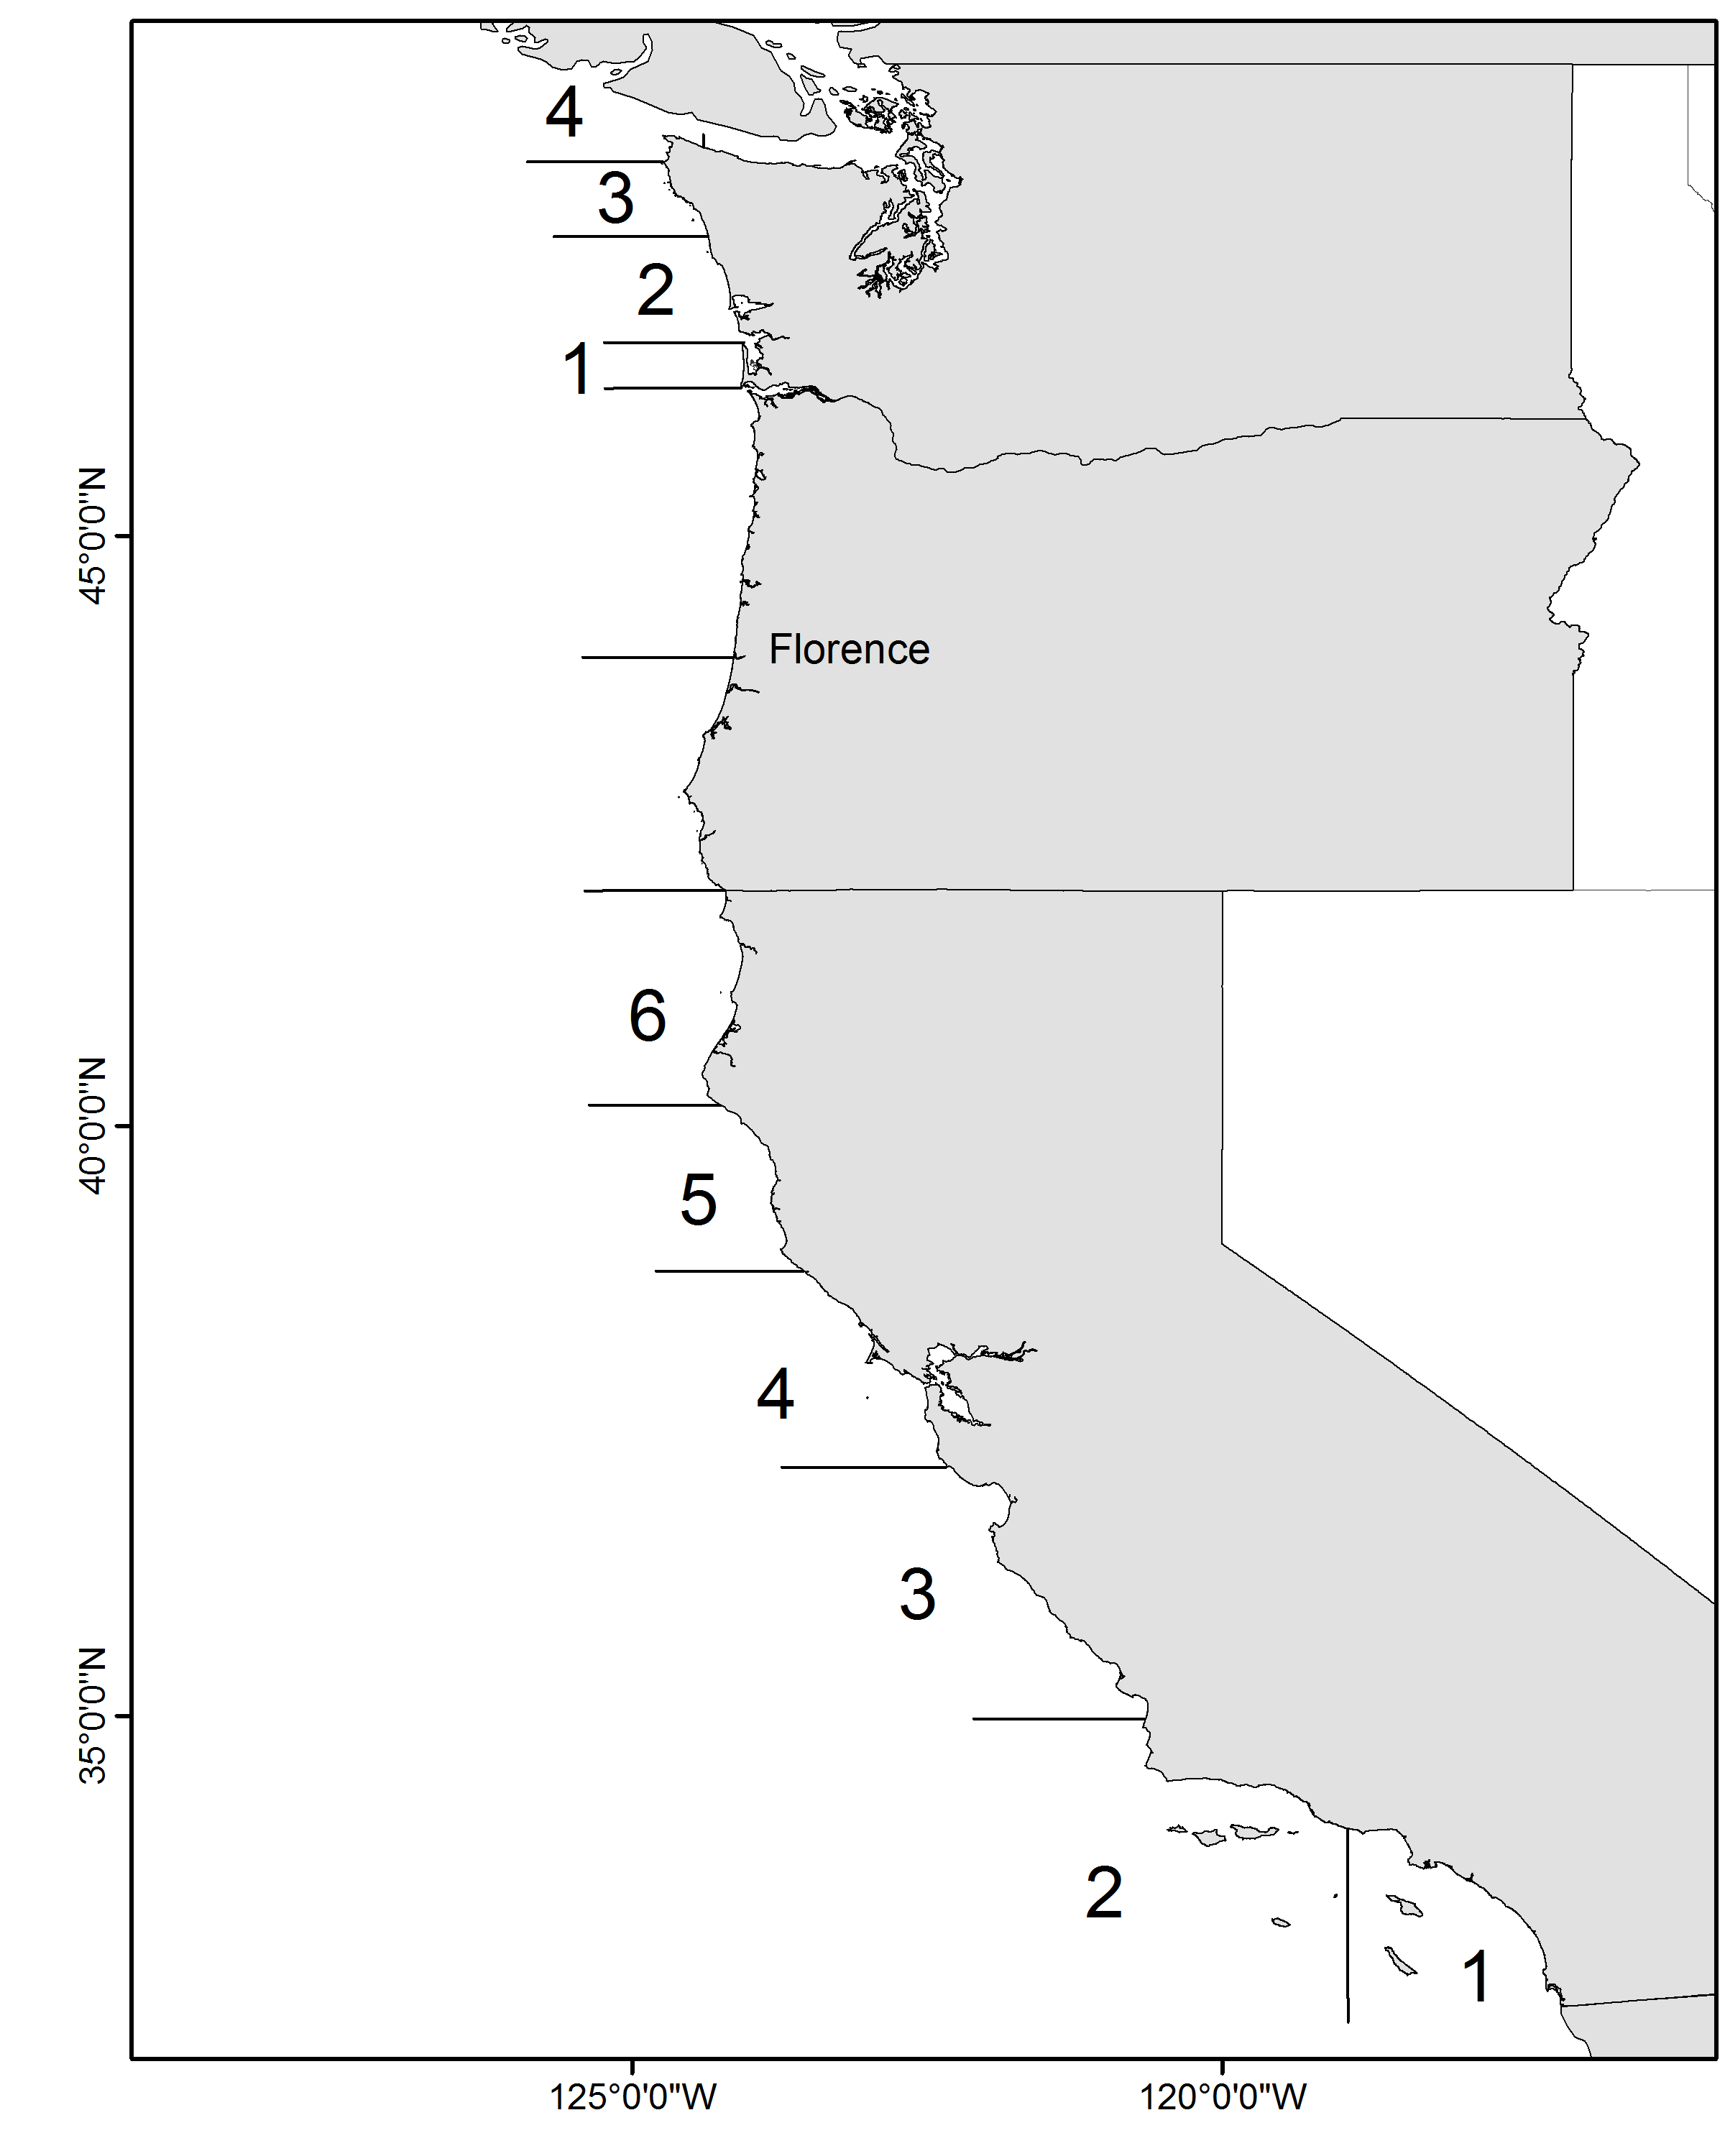
\includegraphics{Figures/boundary_map.png}
\caption{Map showing the state boundary lines for management of the
recreational fishing fleets. CRFS Districts 1-6 in California are
presented as well as the WDFW Recreational Management Areas in
Washington. Florence, OR is shown as a potential location of model
stratification. \label{fig:boundary_map}}
\end{figure}

\begin{figure}
\centering
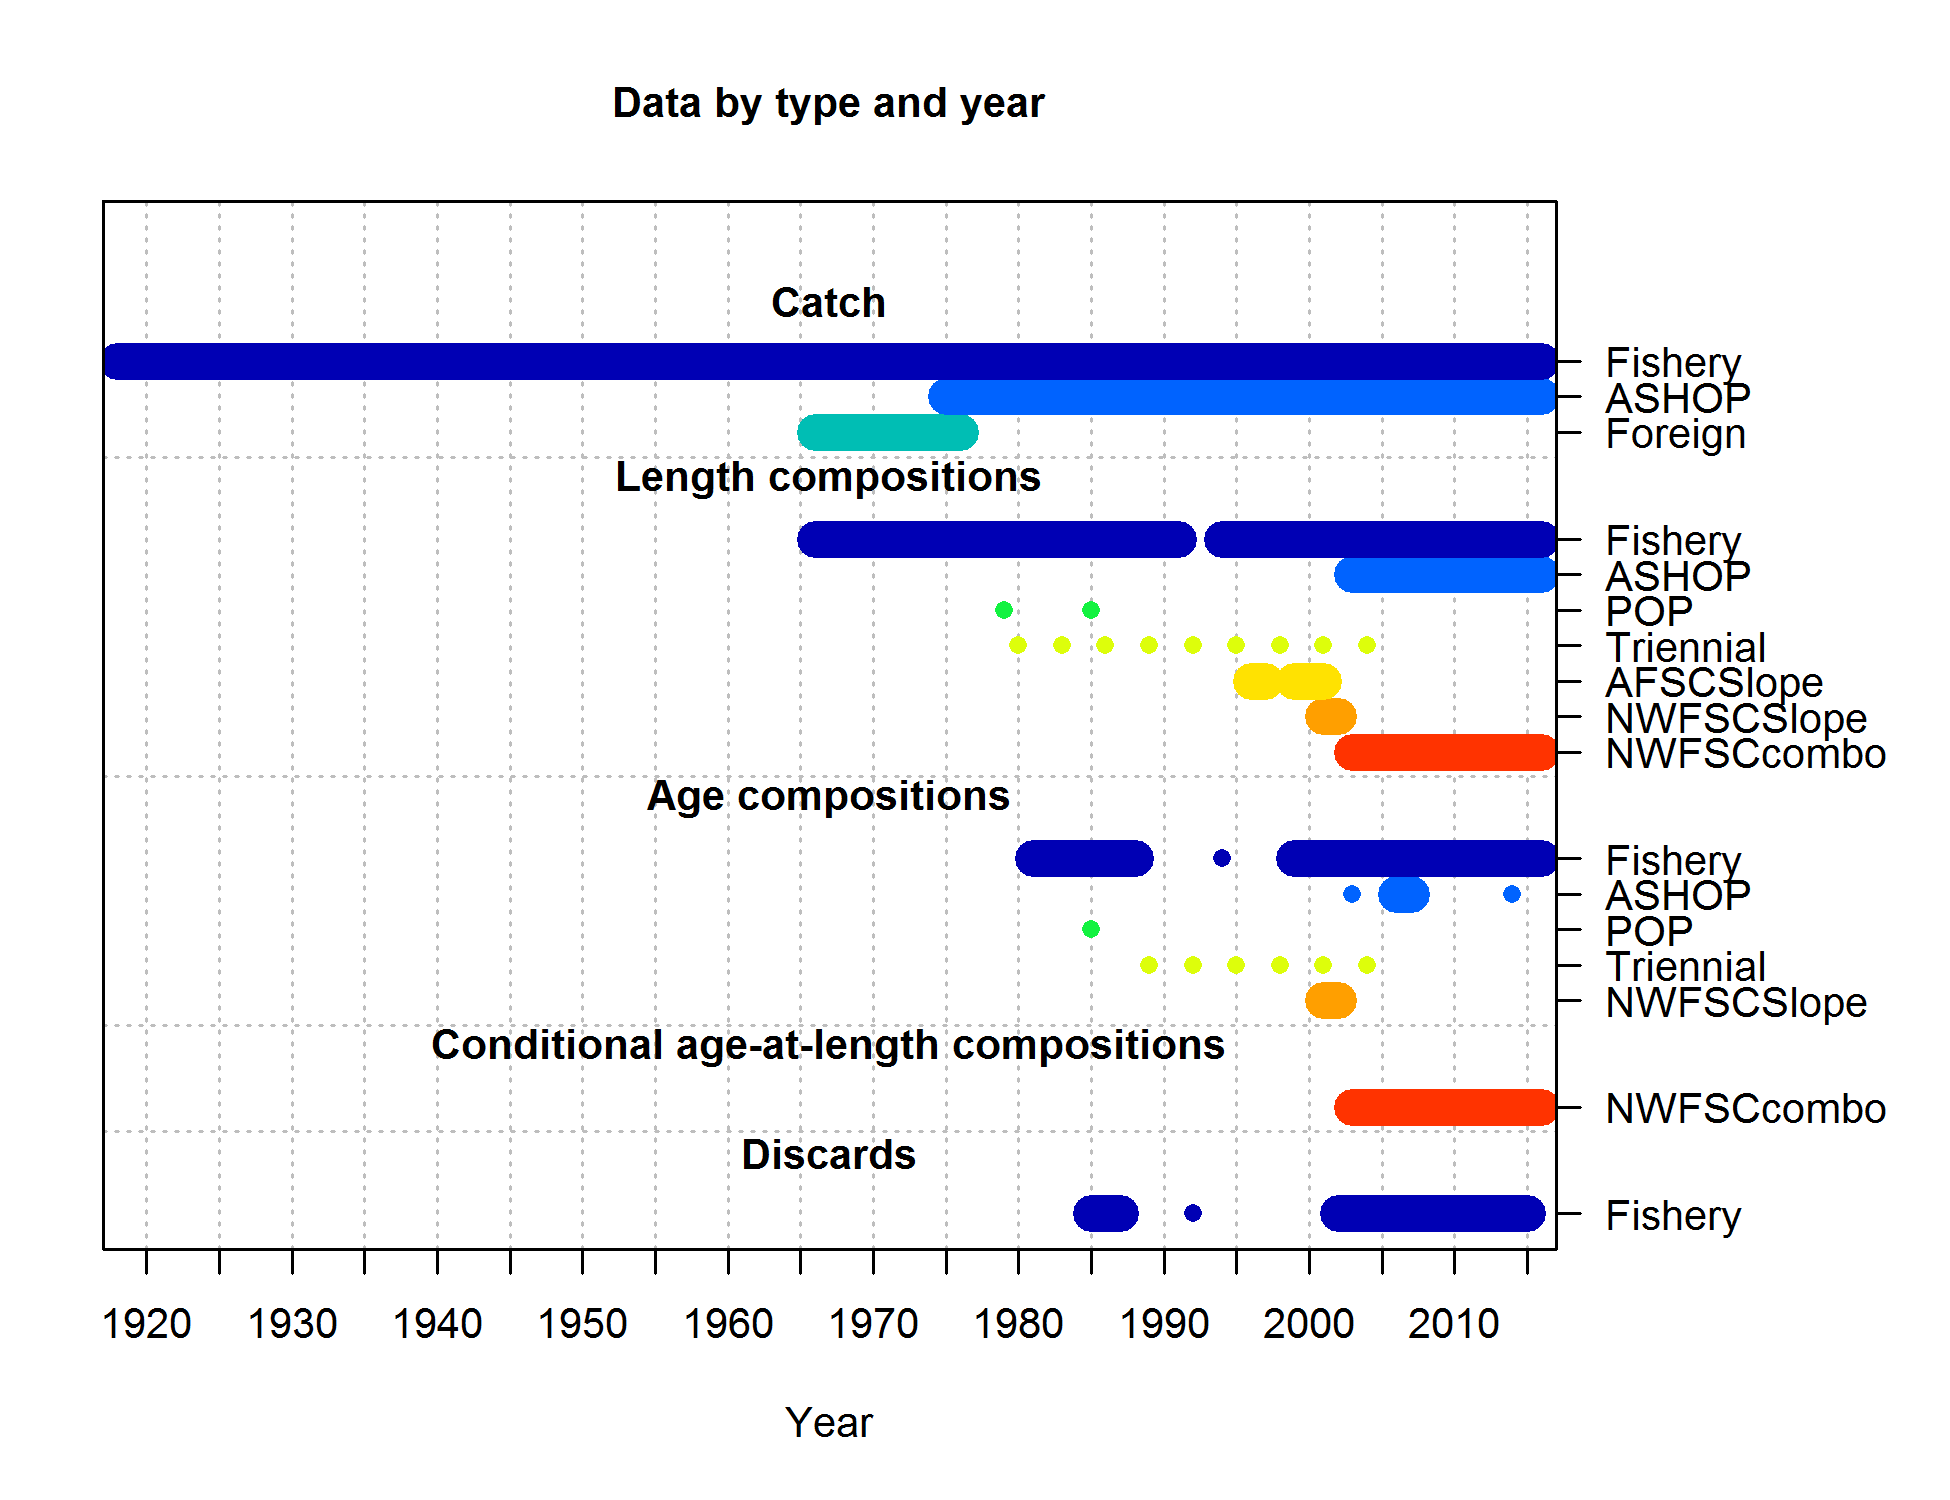
\includegraphics{r4ss/plots_mod1/data_plot.png}
\caption{Summary of data sources used in the Base model.
\label{fig:data_plot}}
\end{figure}

\FloatBarrier

\FloatBarrier

\FloatBarrier

\FloatBarrier

\FloatBarrier

\FloatBarrier

\begin{figure}
\centering
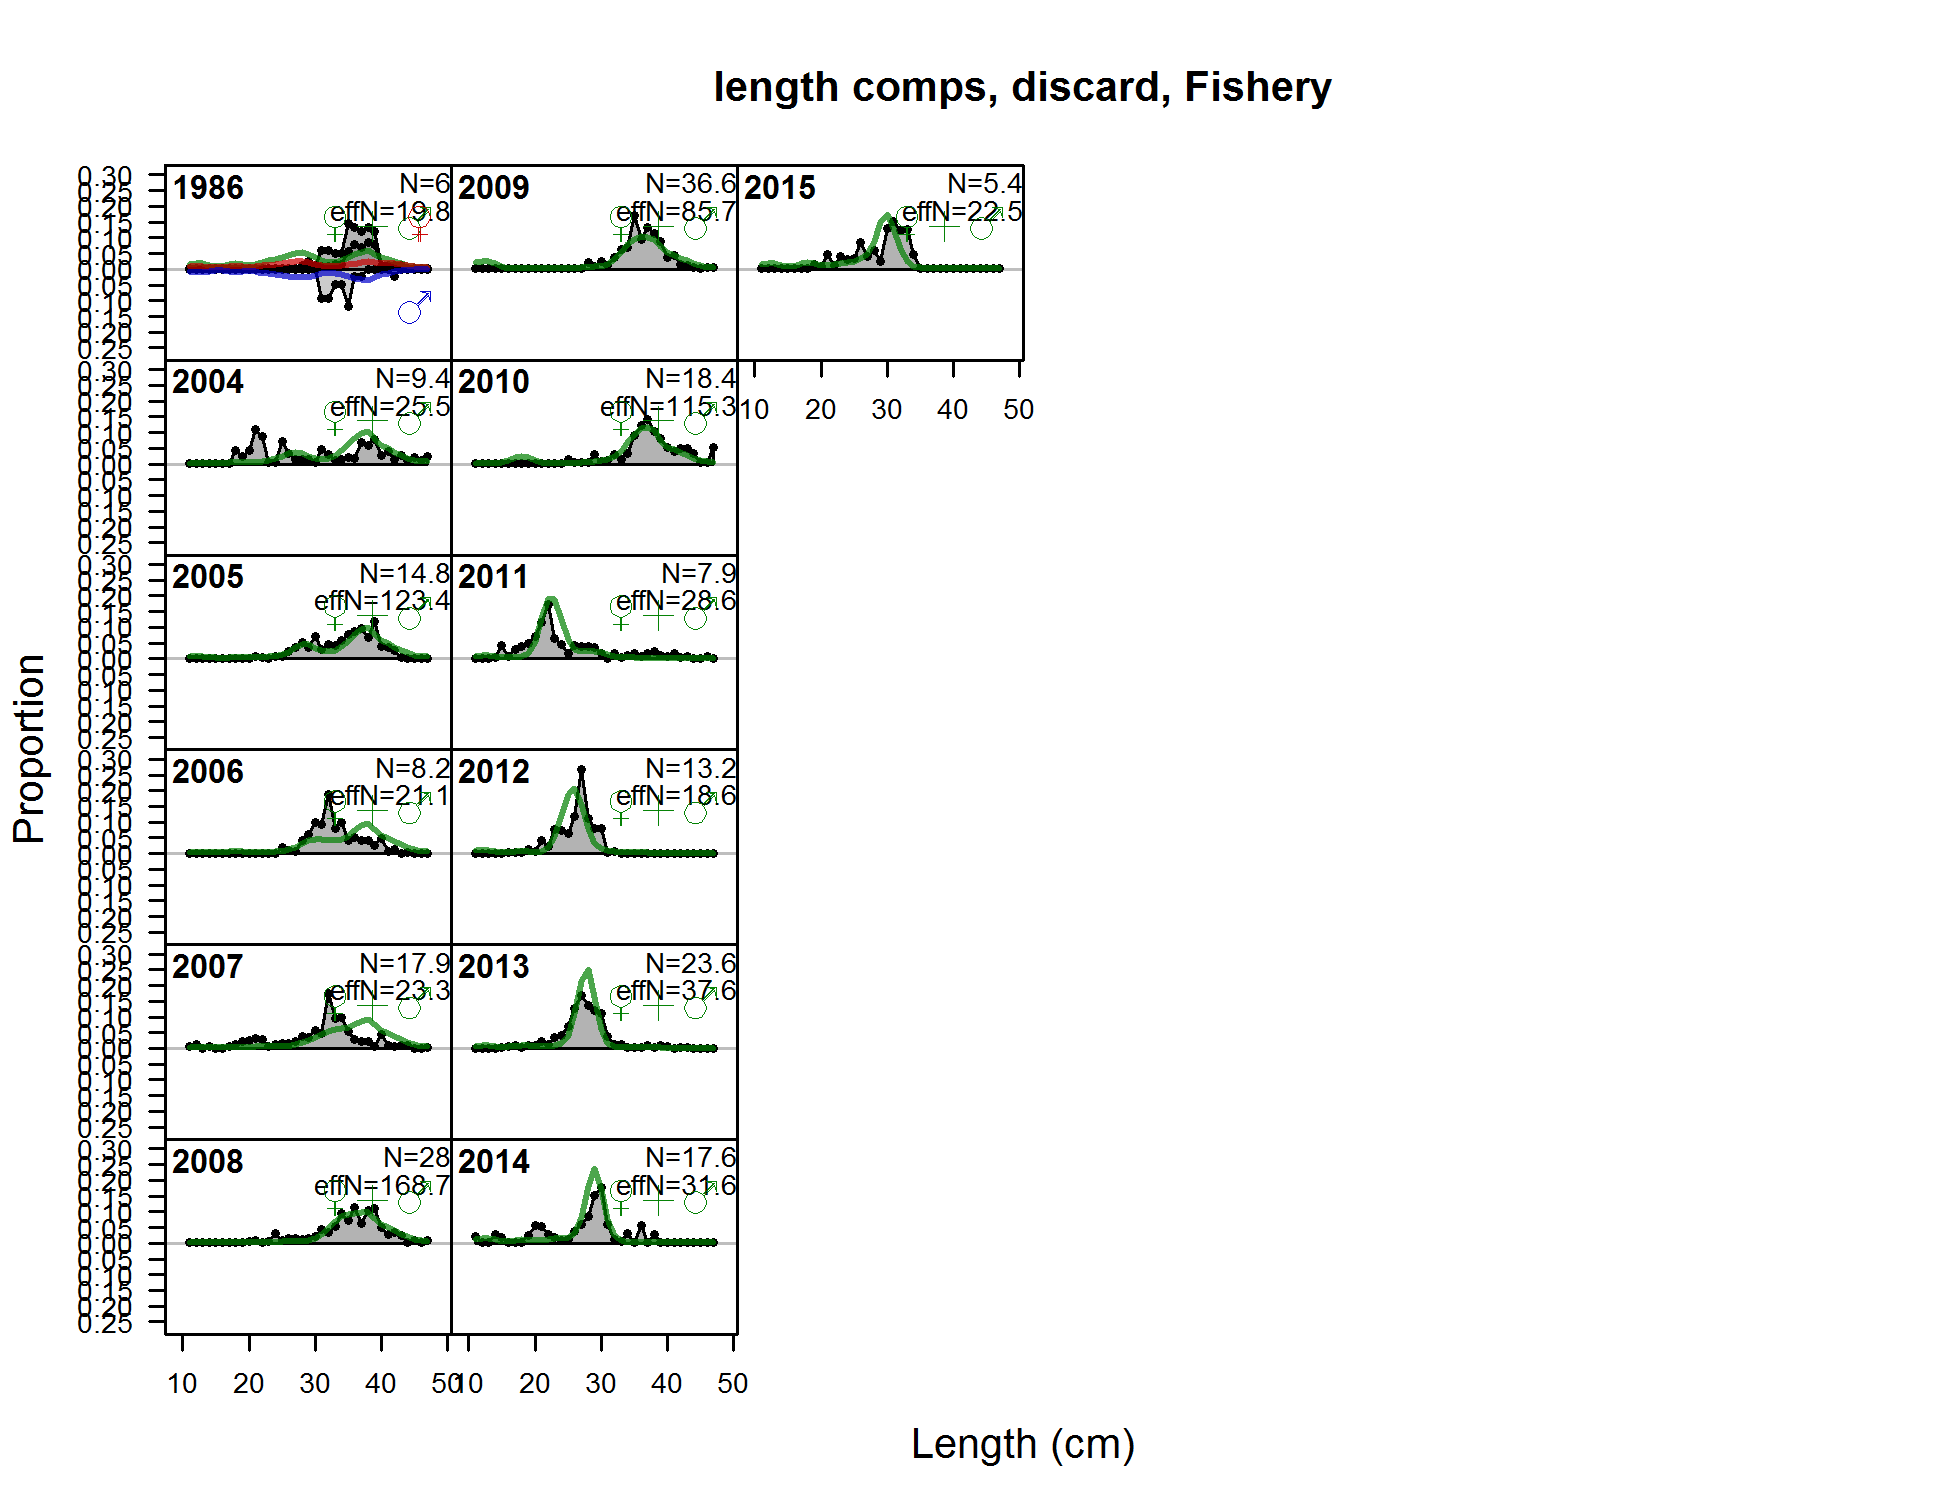
\includegraphics{./r4ss/plots_mod1/comp_lenfit_flt1mkt1.png}
\caption{length comps, discard, Fishery
\label{fig:mod1_1_comp_lenfit_flt1mkt1}}
\end{figure}

\begin{figure}
\centering
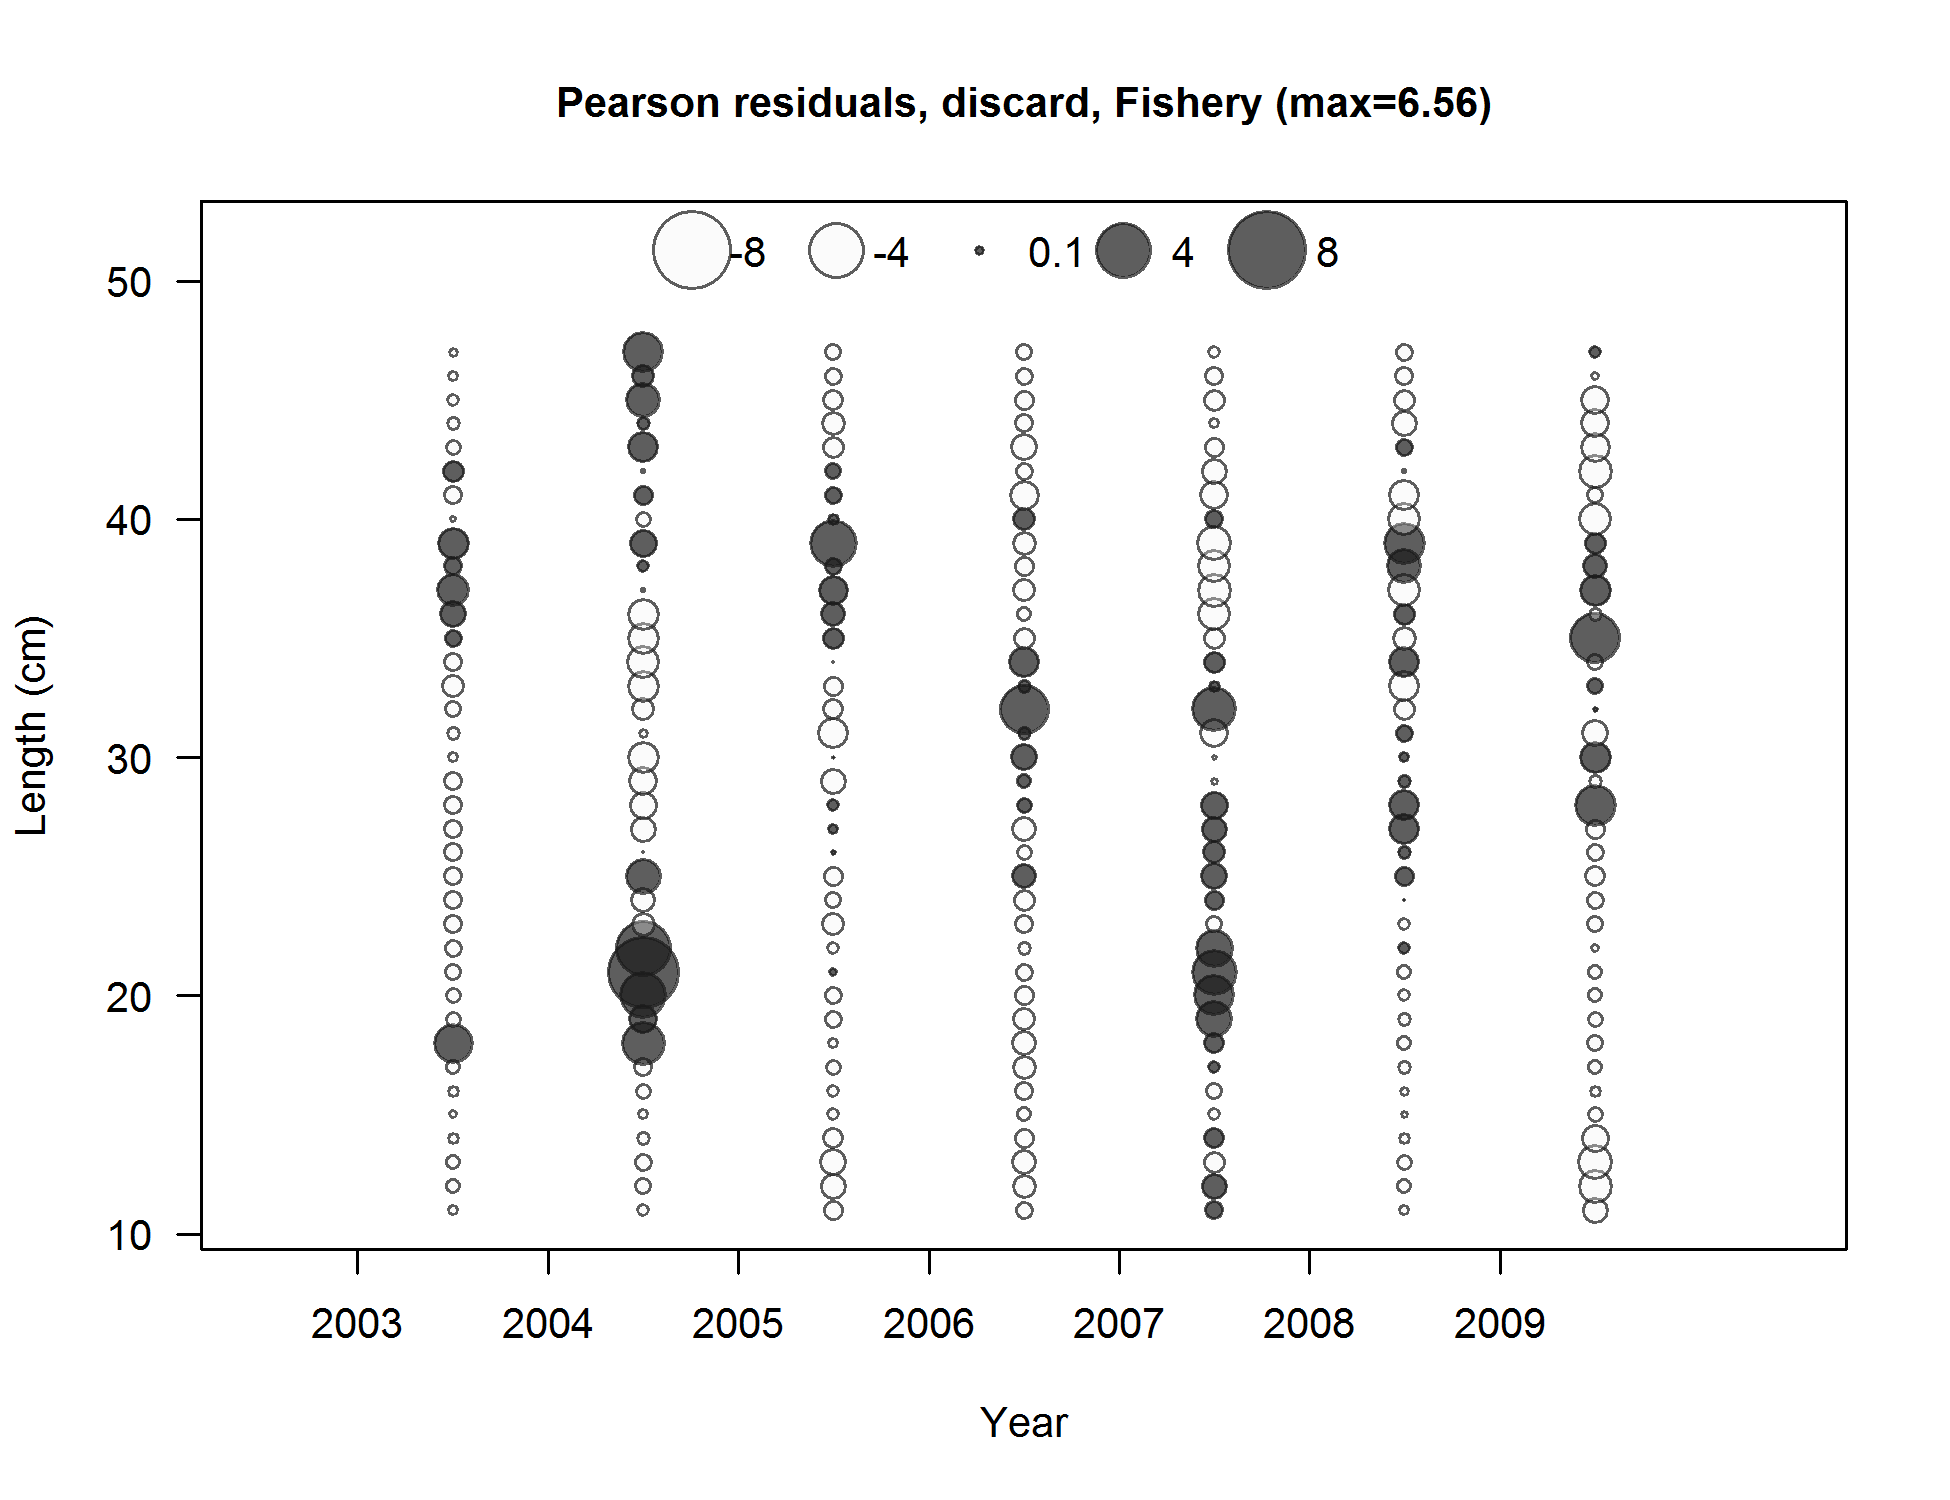
\includegraphics{./r4ss/plots_mod1/comp_lenfit_residsflt1mkt1.png}
\caption{Pearson residuals, discard, Fishery (max=6.5)\\
Closed bubbles are positive residuals (observed \textgreater{} expected)
and open bubbles are negative residuals (observed \textless{} expected).
\label{fig:mod1_2_comp_lenfit_residsflt1mkt1}}
\end{figure}

\begin{figure}
\centering
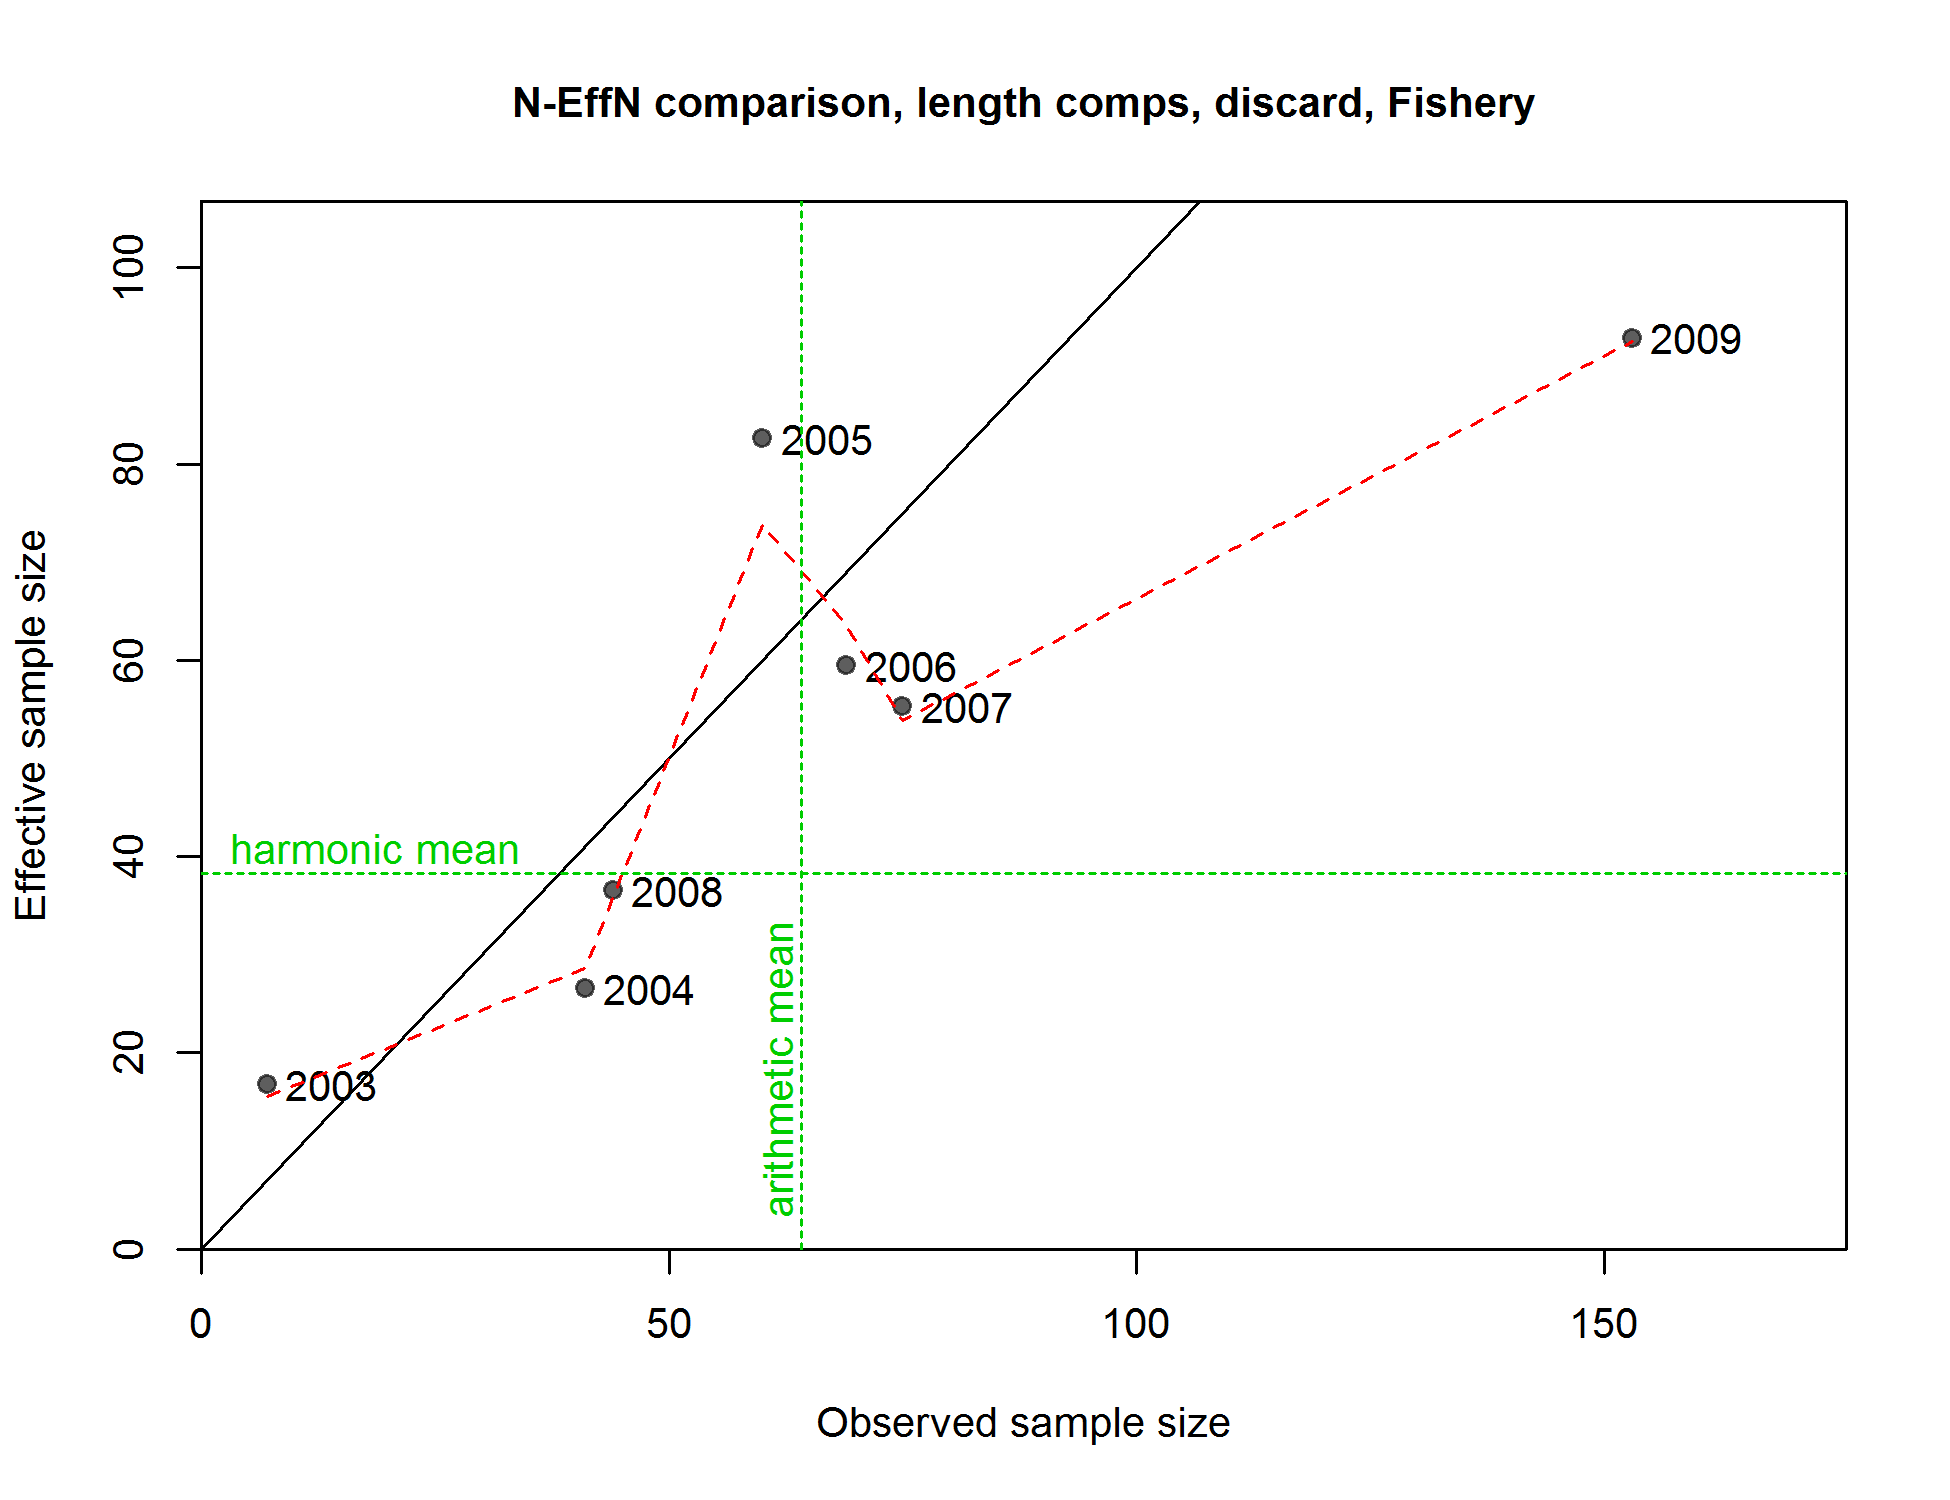
\includegraphics{./r4ss/plots_mod1/comp_lenfit_sampsize_flt1mkt1.png}
\caption{N\_EffN comparison, length comps, discard, Fishery
\label{fig:mod1_3_comp_lenfit_sampsize_flt1mkt1}}
\end{figure}

\begin{figure}
\centering
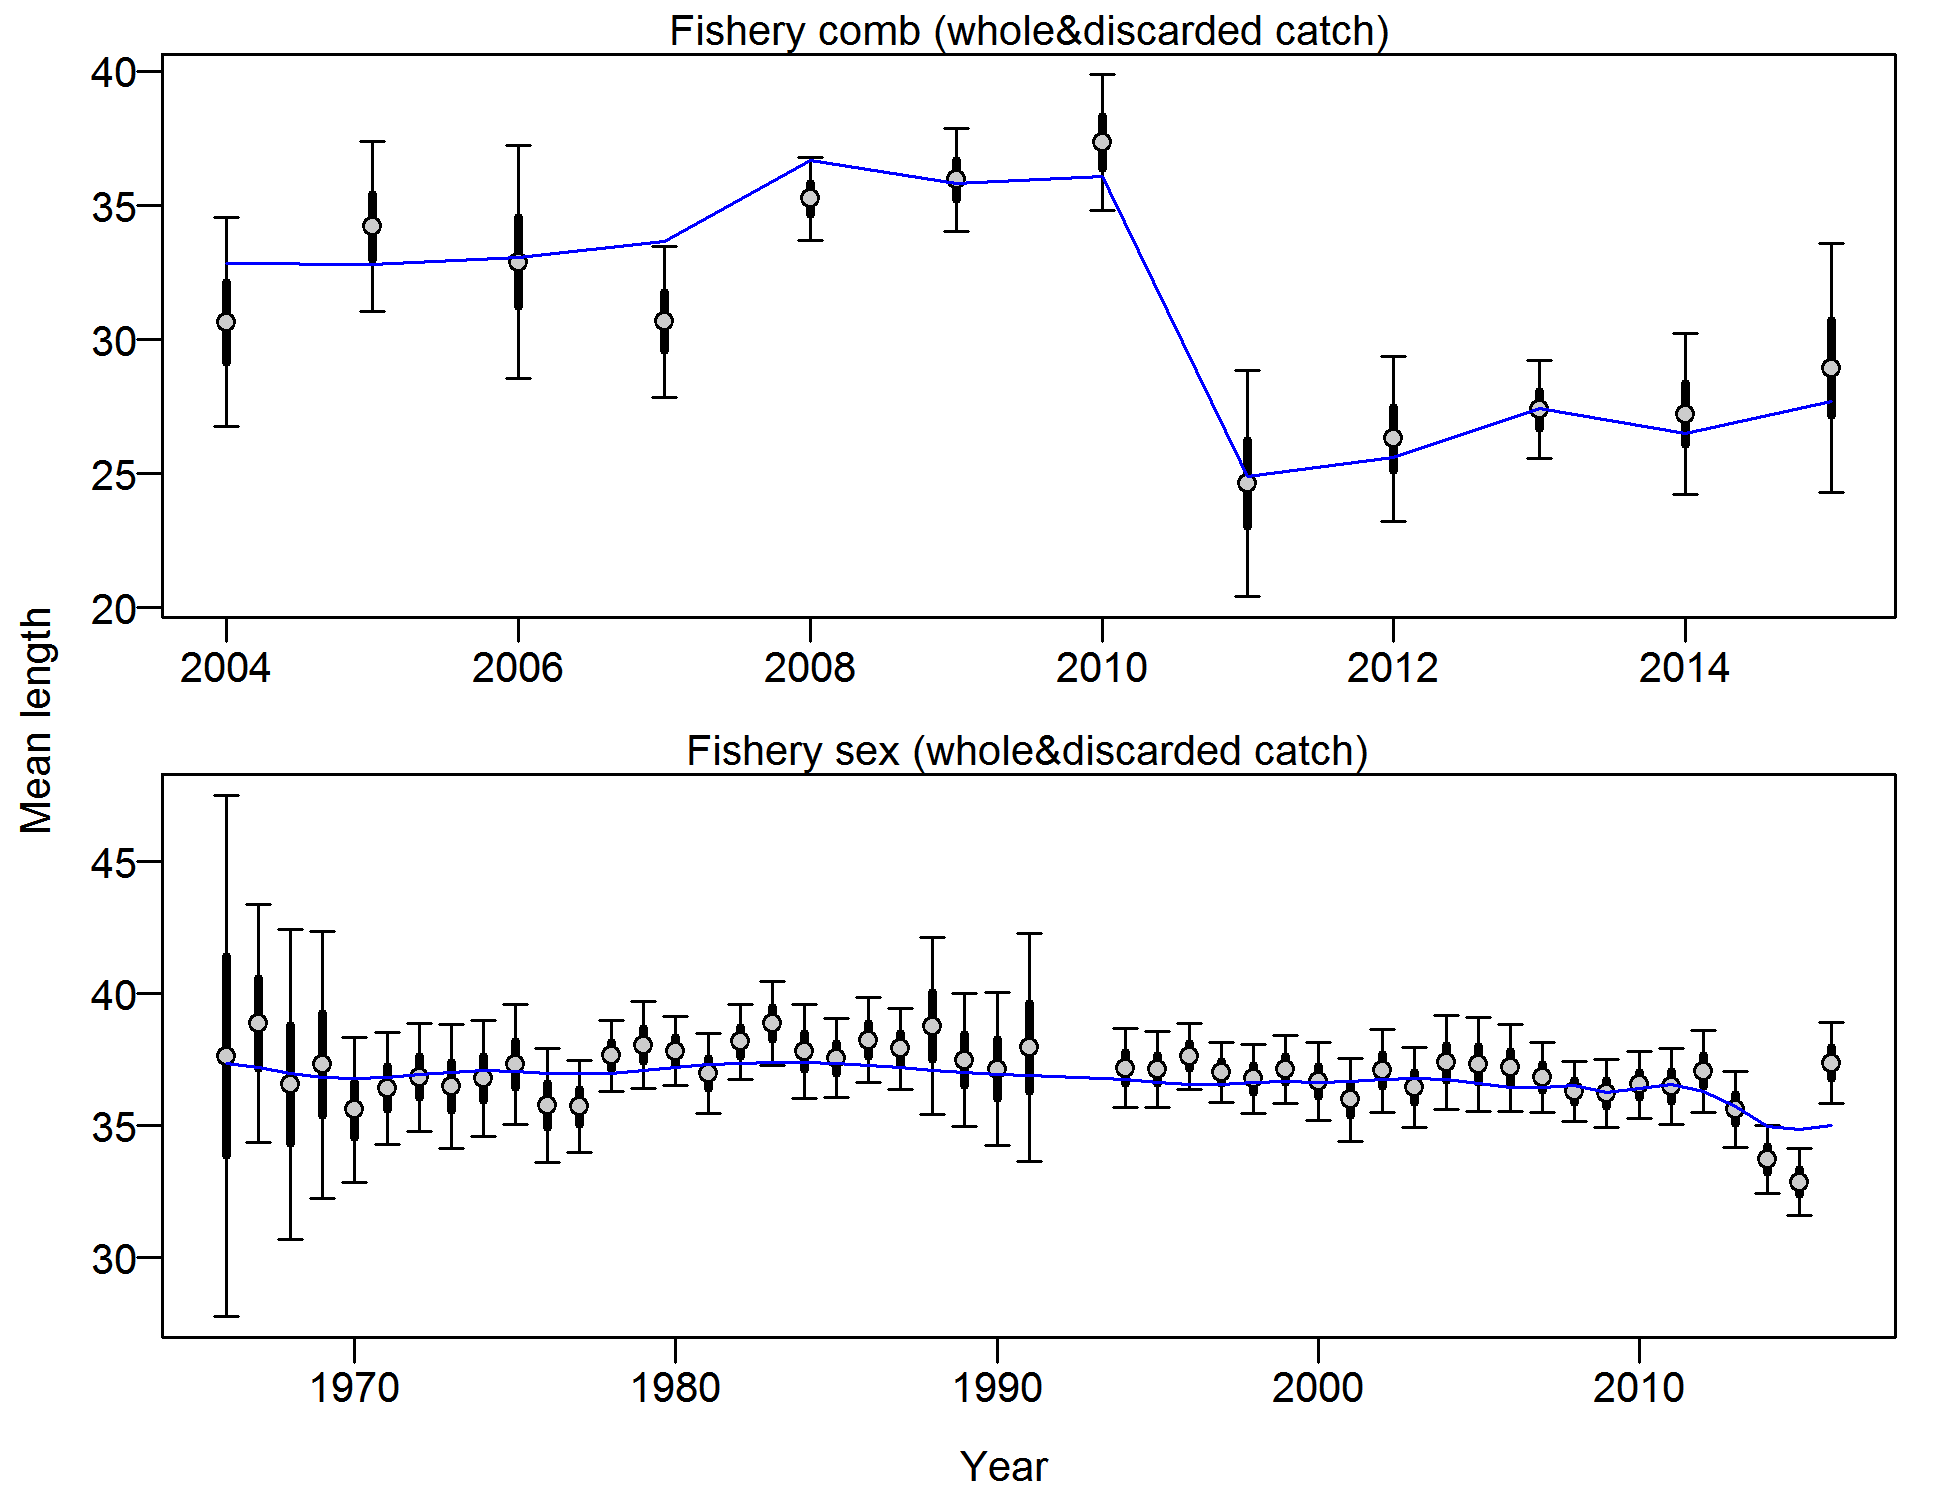
\includegraphics{./r4ss/plots_mod1/comp_lenfit_data_weighting_TA1.8_Fishery.png}
\caption{Francis data weighting method TA1.8 Fishery Suggested sample
size adjustment (with 95\% interval) for len data from Fishery: 0.2517
(0.1563\_0.5907)
\label{fig:mod1_4_comp_lenfit_data_weighting_TA1.8_Fishery}}
\end{figure}

\begin{figure}
\centering
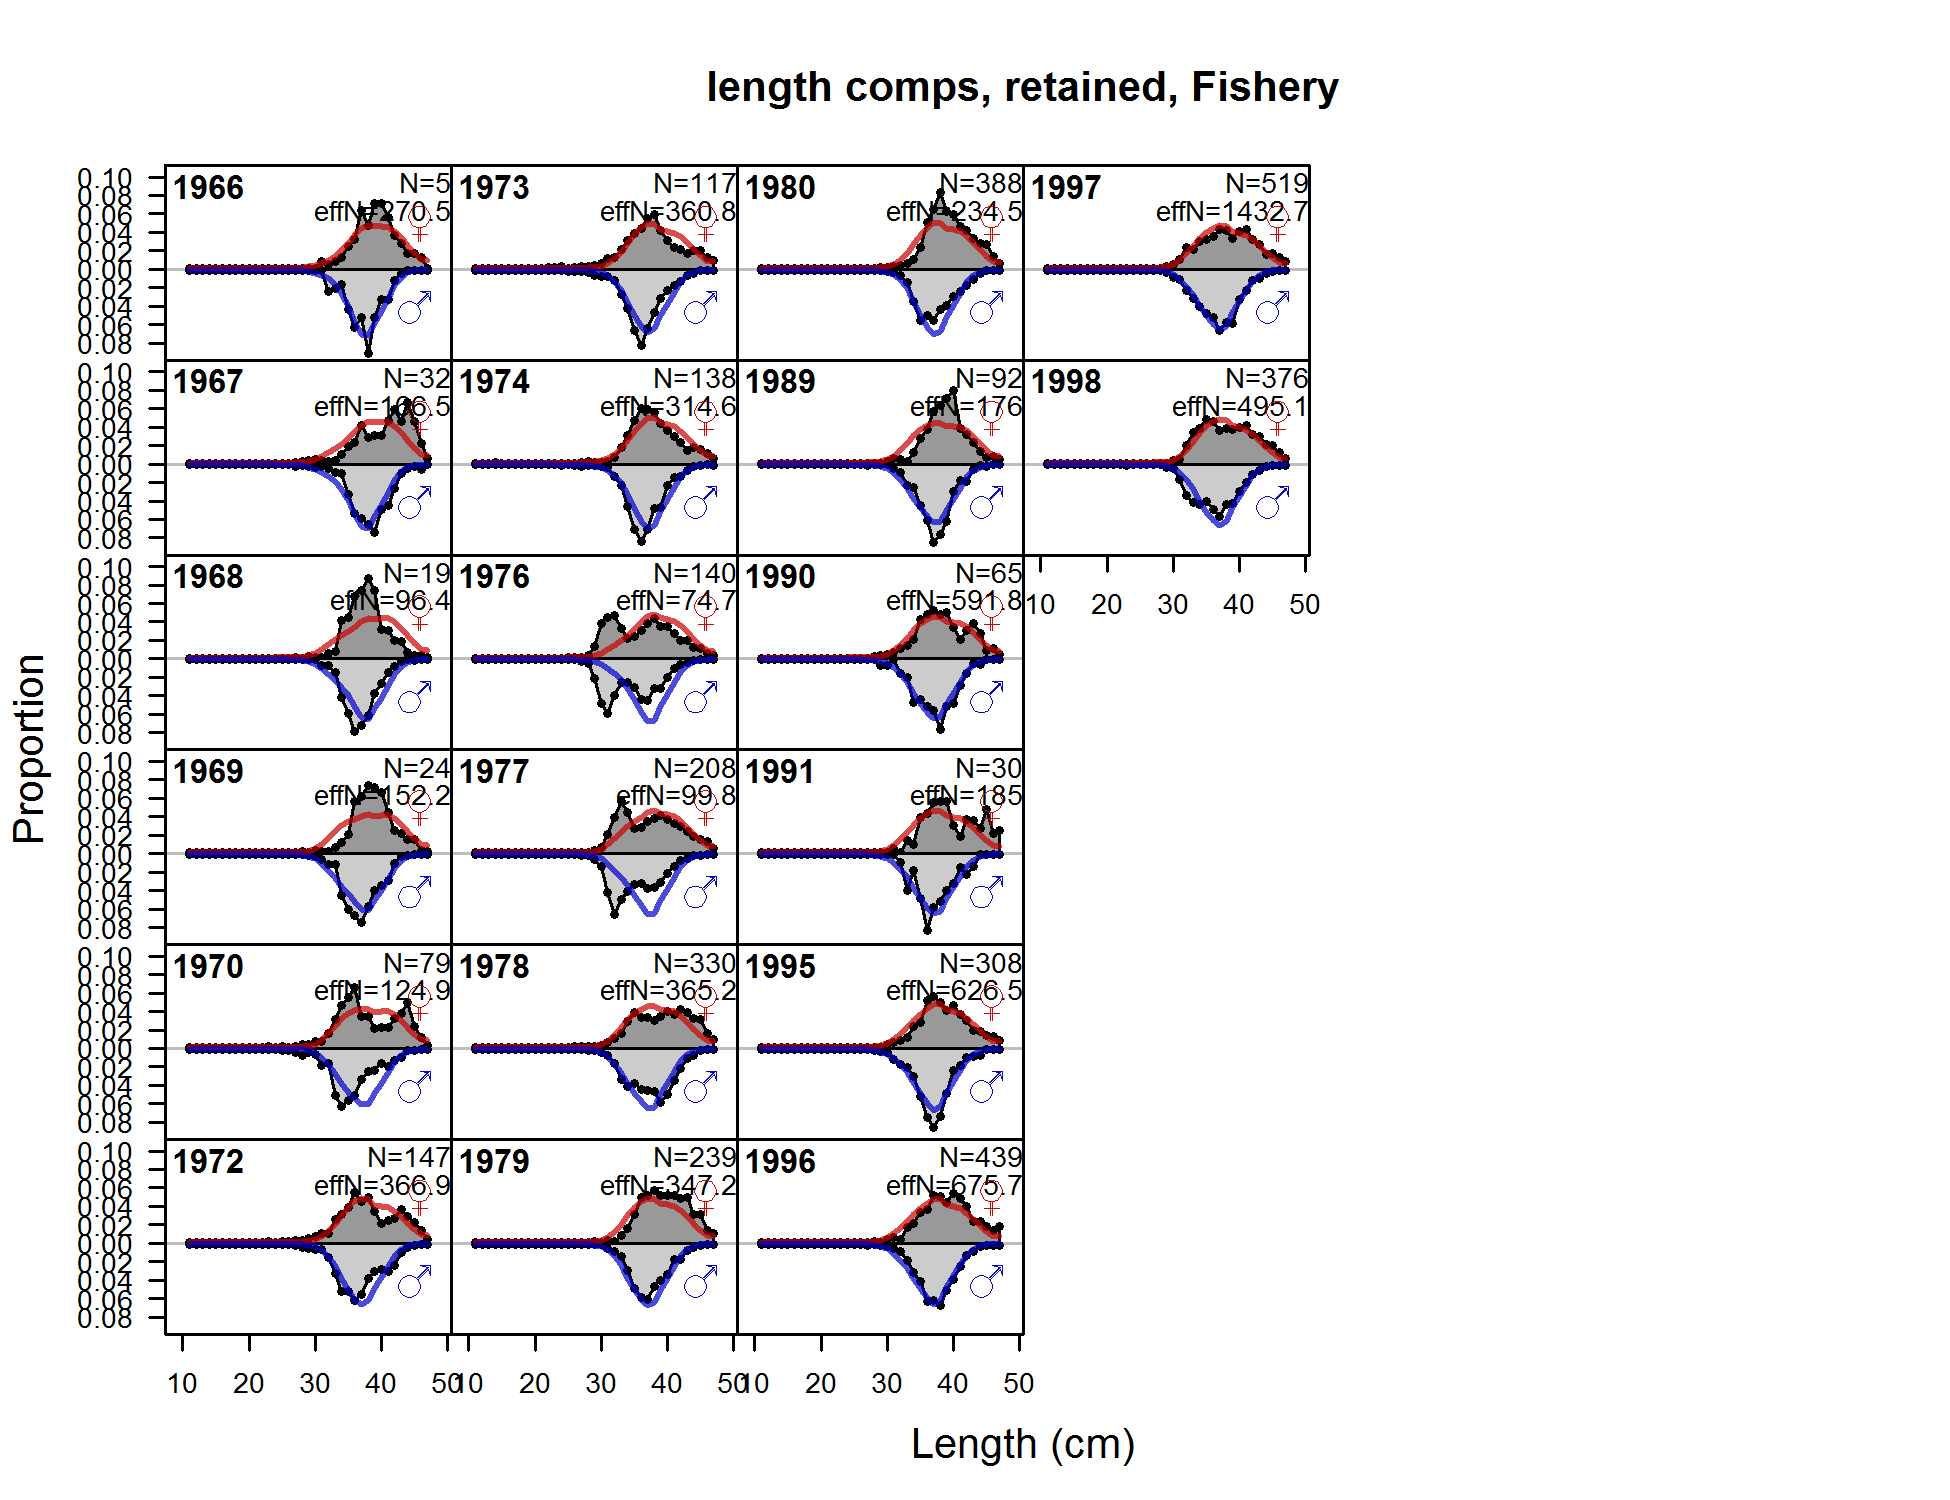
\includegraphics{./r4ss/plots_mod1/comp_lenfit_flt1mkt2.png}
\caption{length comps, retained, Fishery
\label{fig:mod1_5_comp_lenfit_flt1mkt2}}
\end{figure}

\begin{figure}
\centering
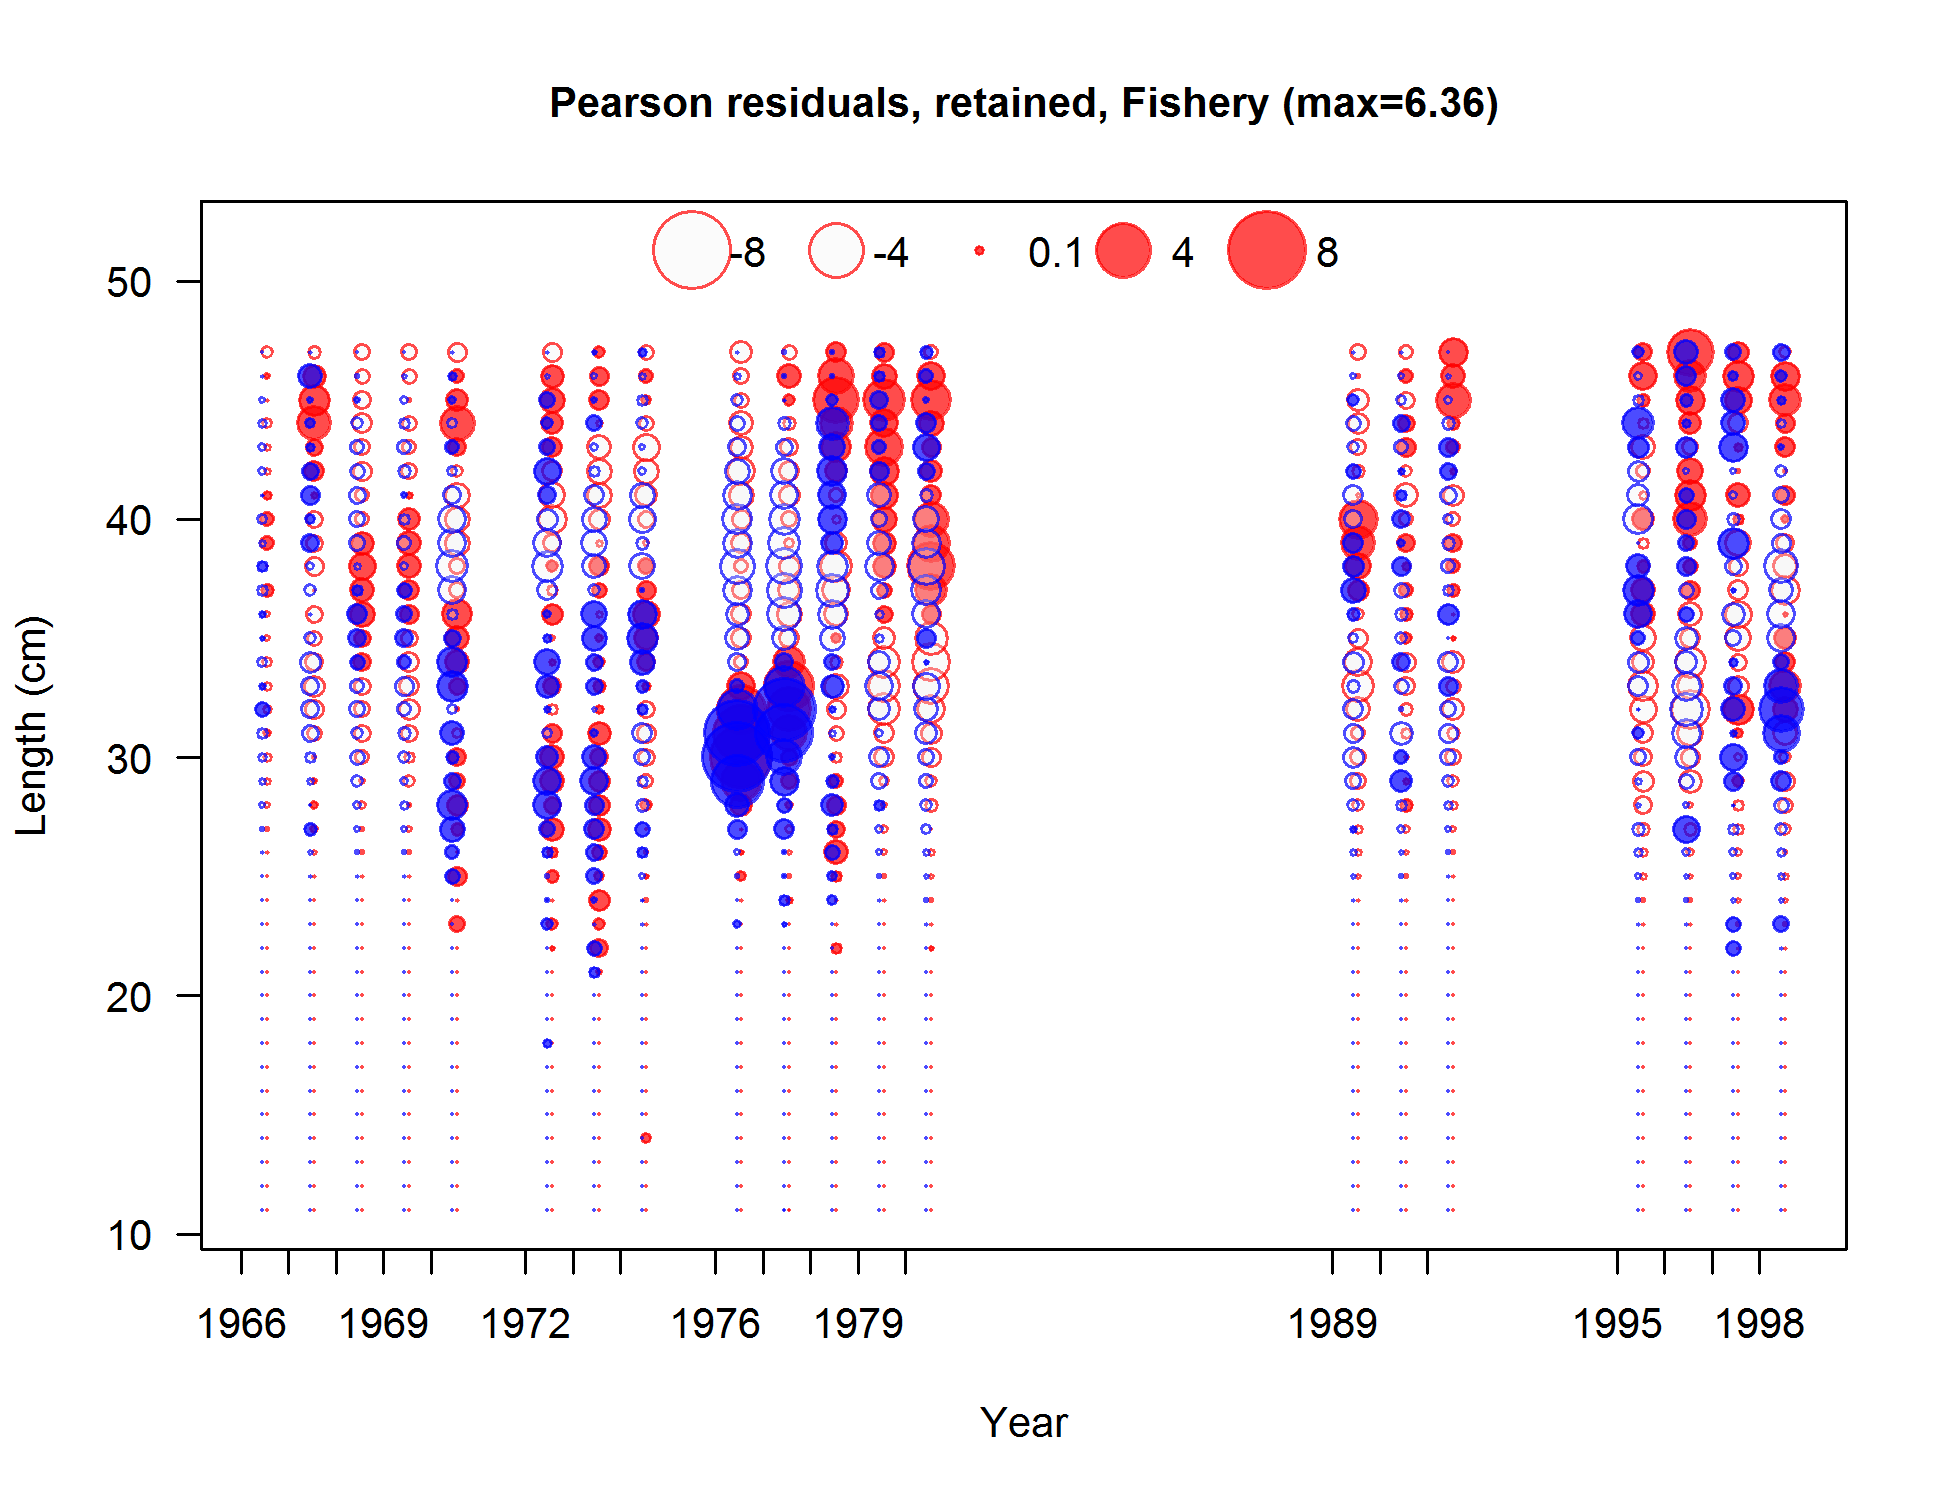
\includegraphics{./r4ss/plots_mod1/comp_lenfit_residsflt1mkt2.png}
\caption{Pearson residuals, retained, Fishery (max=6.3)\\
Closed bubbles are positive residuals (observed \textgreater{} expected)
and open bubbles are negative residuals (observed \textless{} expected).
\label{fig:mod1_6_comp_lenfit_residsflt1mkt2}}
\end{figure}

\begin{figure}
\centering
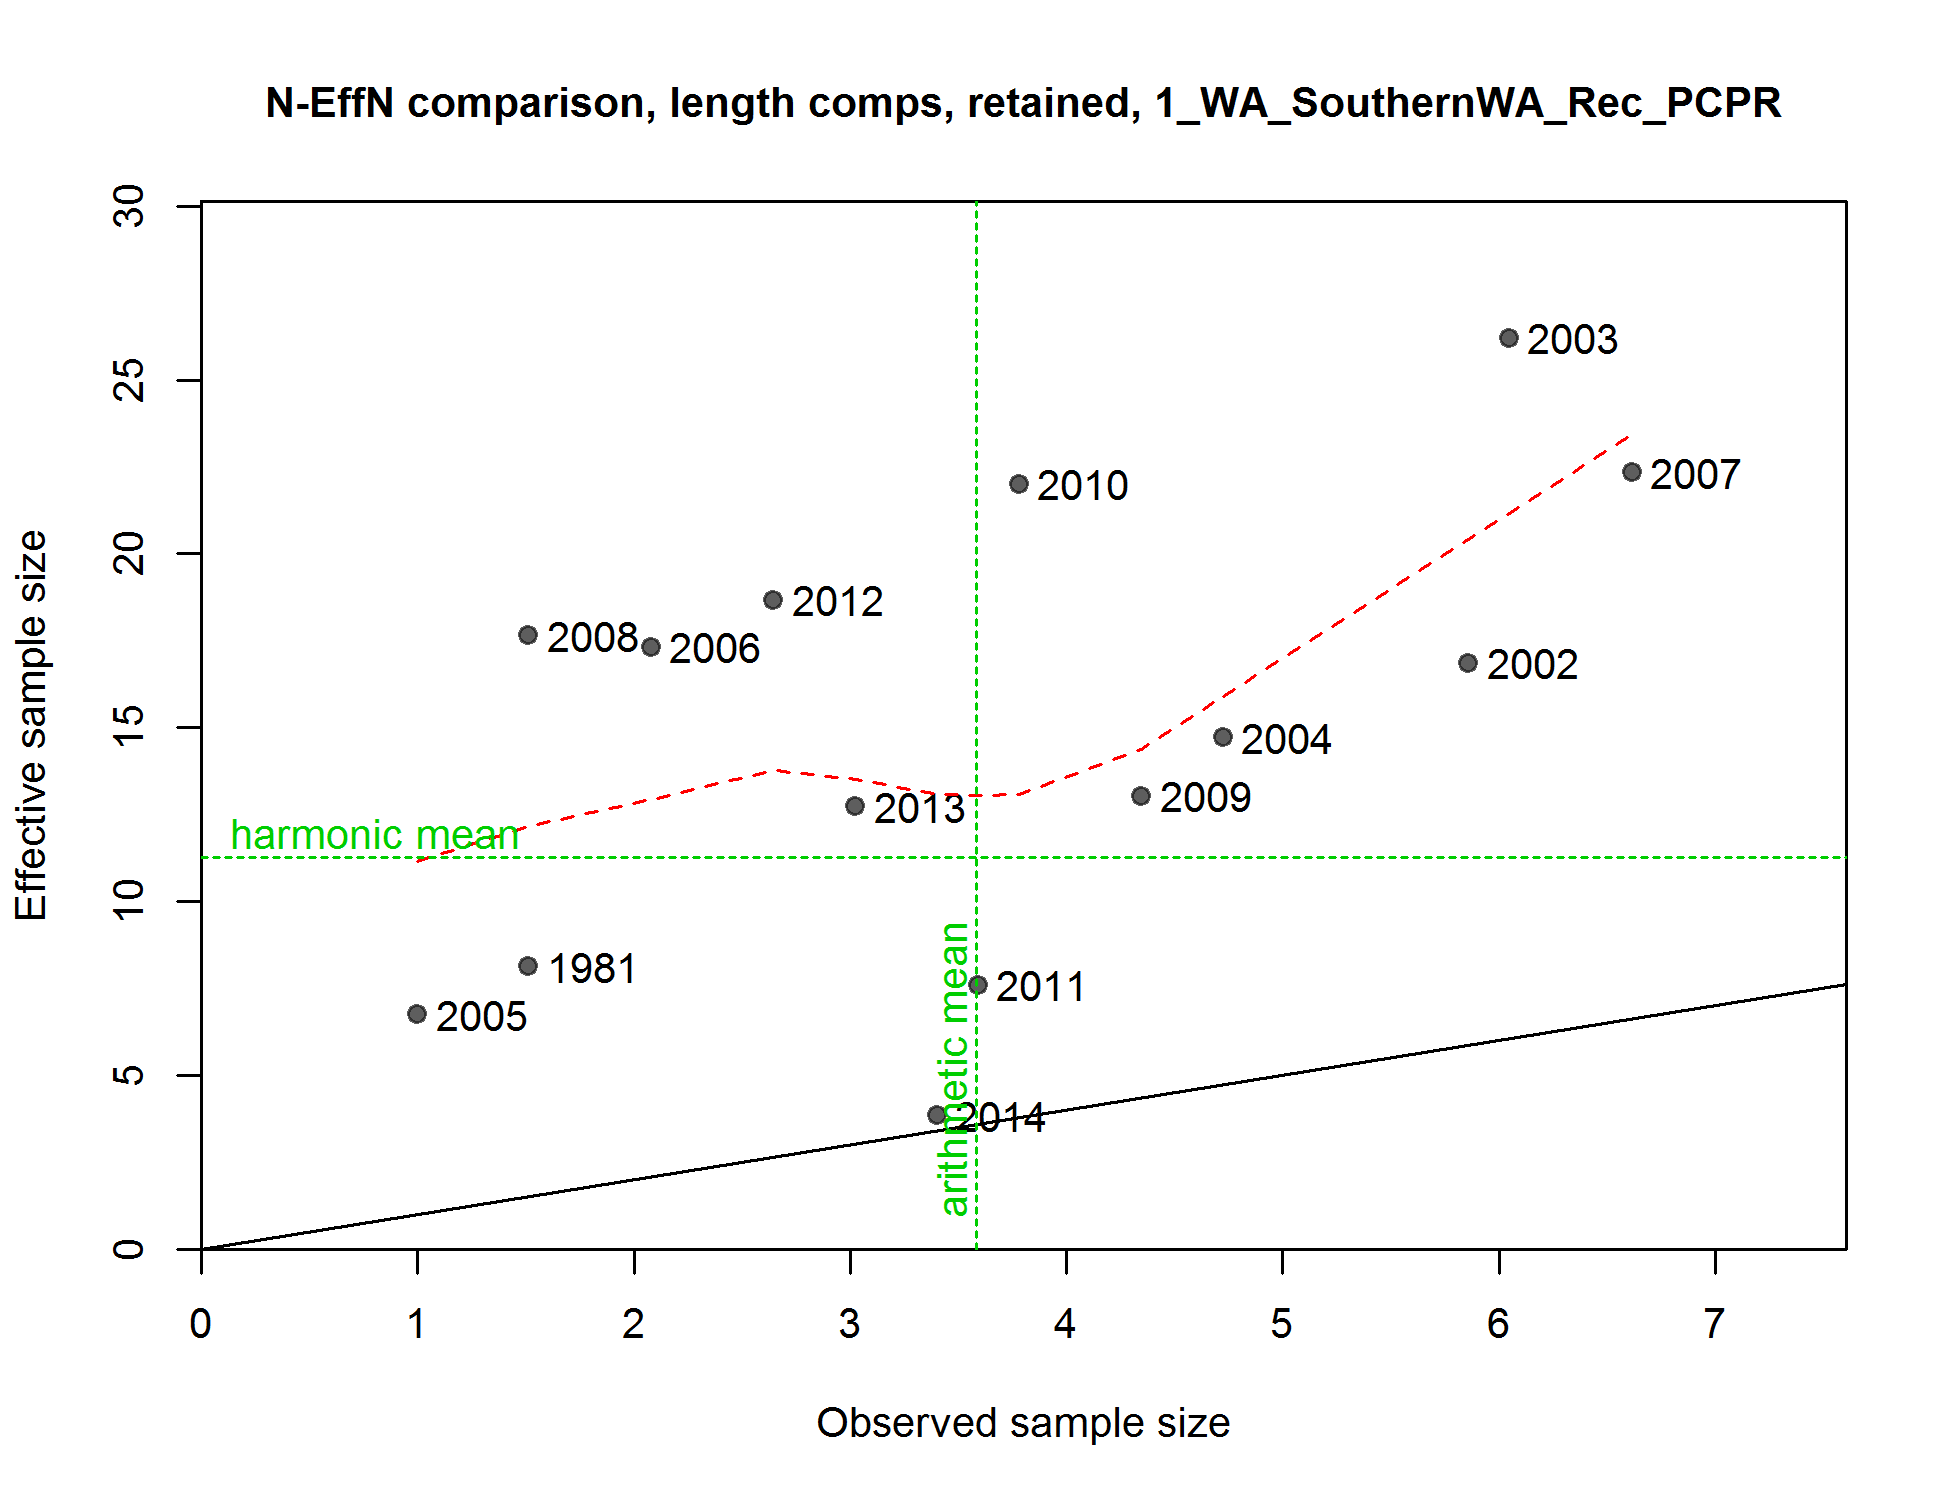
\includegraphics{./r4ss/plots_mod1/comp_lenfit_sampsize_flt1mkt2.png}
\caption{N\_EffN comparison, length comps, retained, Fishery
\label{fig:mod1_7_comp_lenfit_sampsize_flt1mkt2}}
\end{figure}

\begin{figure}
\centering
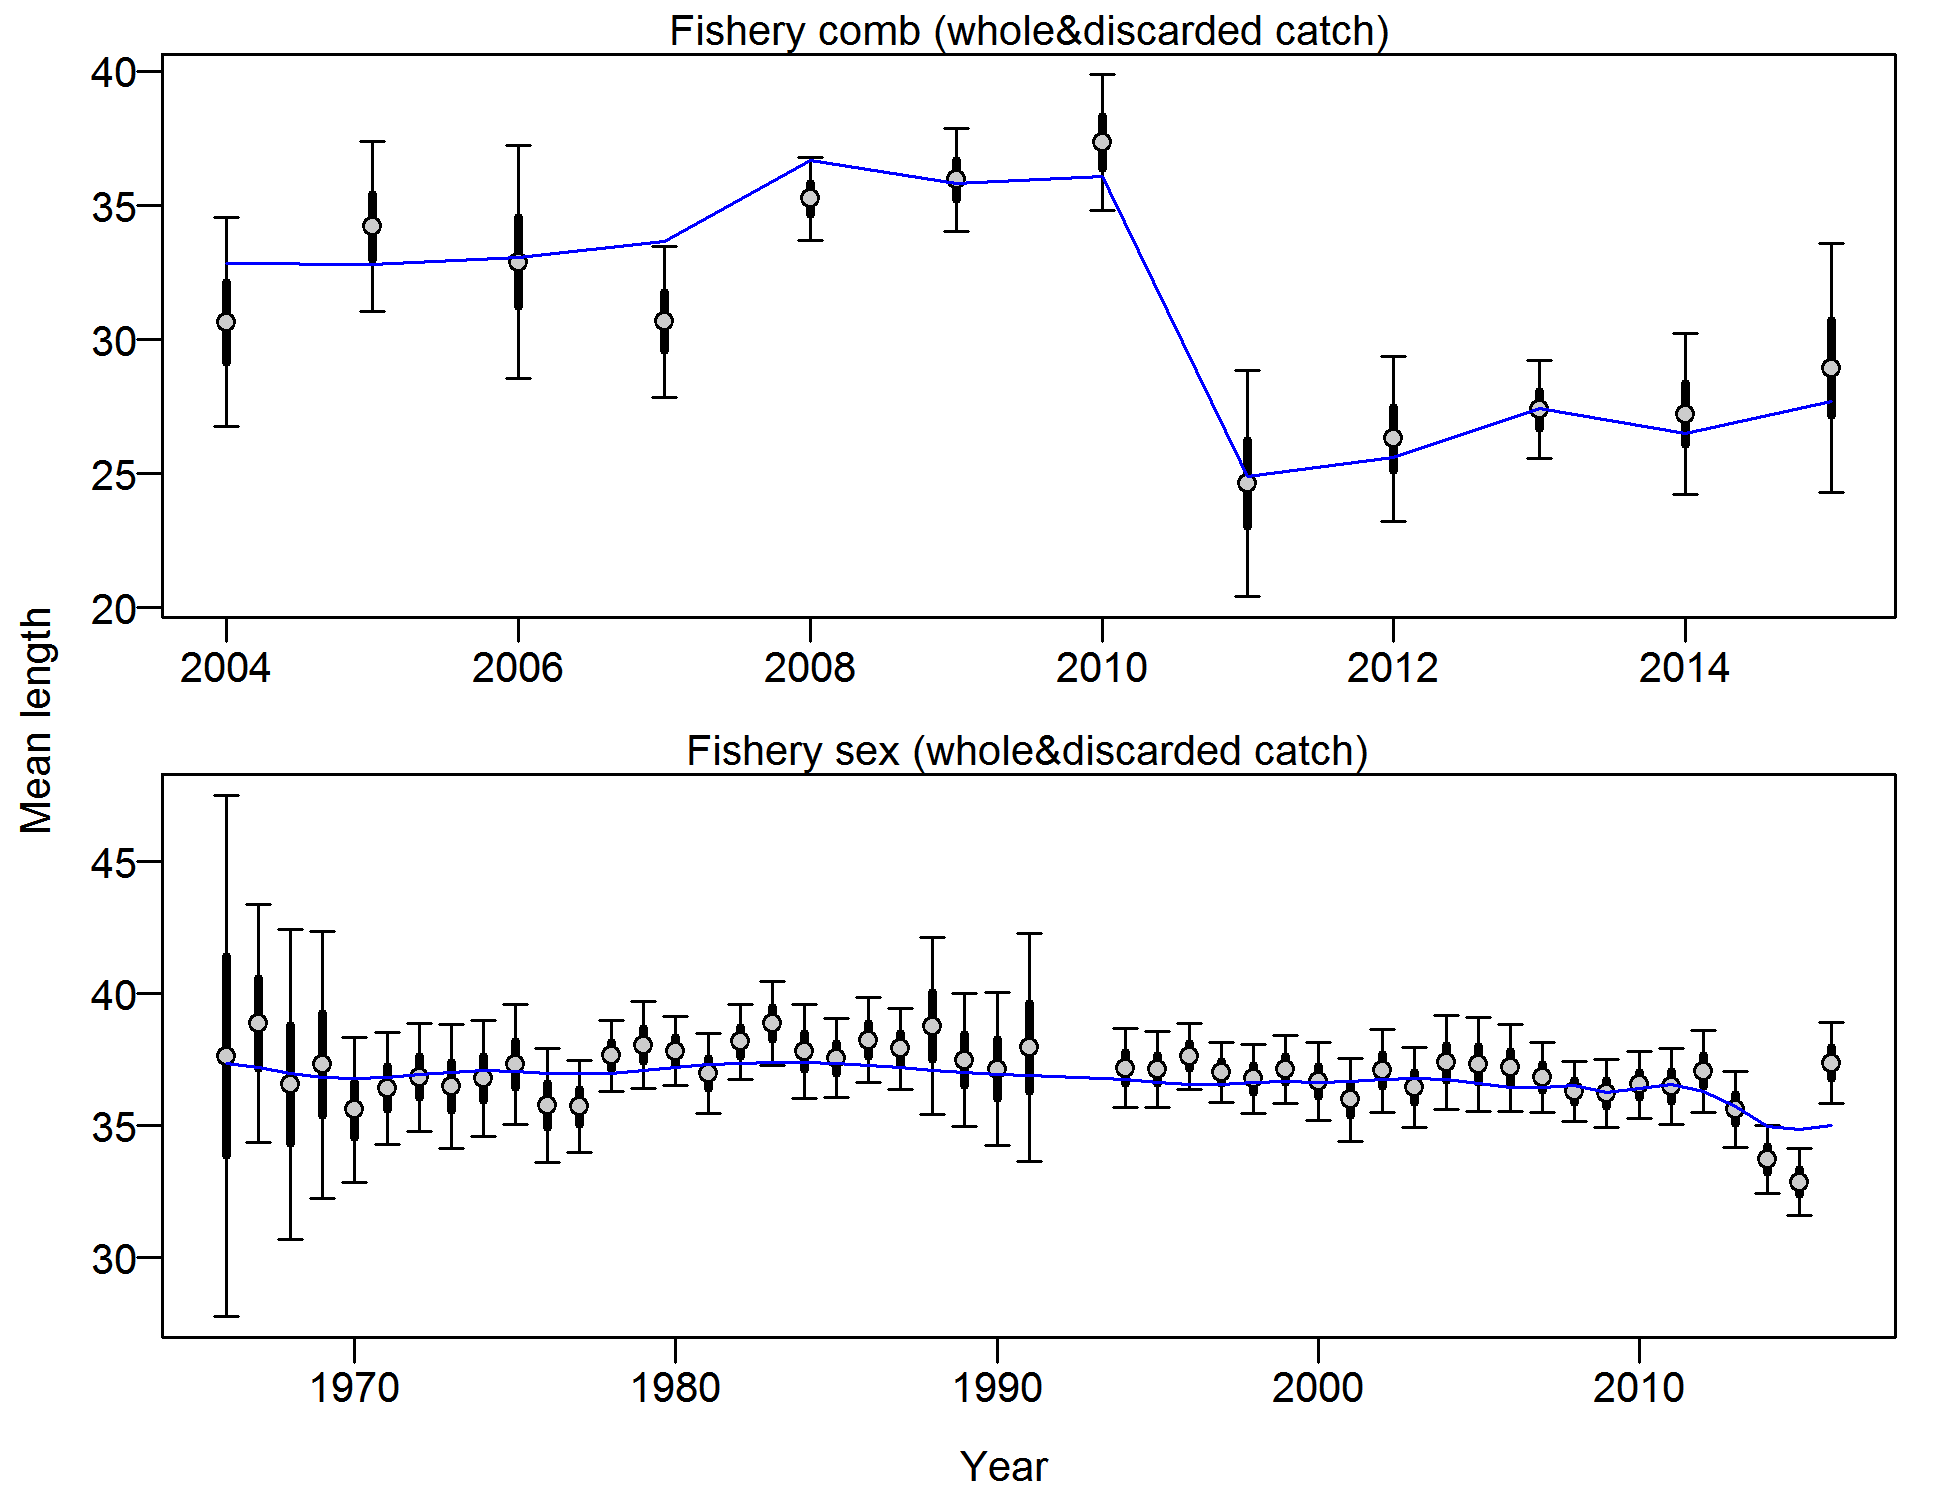
\includegraphics{./r4ss/plots_mod1/comp_lenfit_data_weighting_TA1.8_Fishery.png}
\caption{Francis data weighting method TA1.8 Fishery Suggested sample
size adjustment (with 95\% interval) for len data from Fishery: 0.2517
(0.1586\_0.5848)
\label{fig:mod1_8_comp_lenfit_data_weighting_TA1.8_Fishery}}
\end{figure}

\begin{figure}
\centering
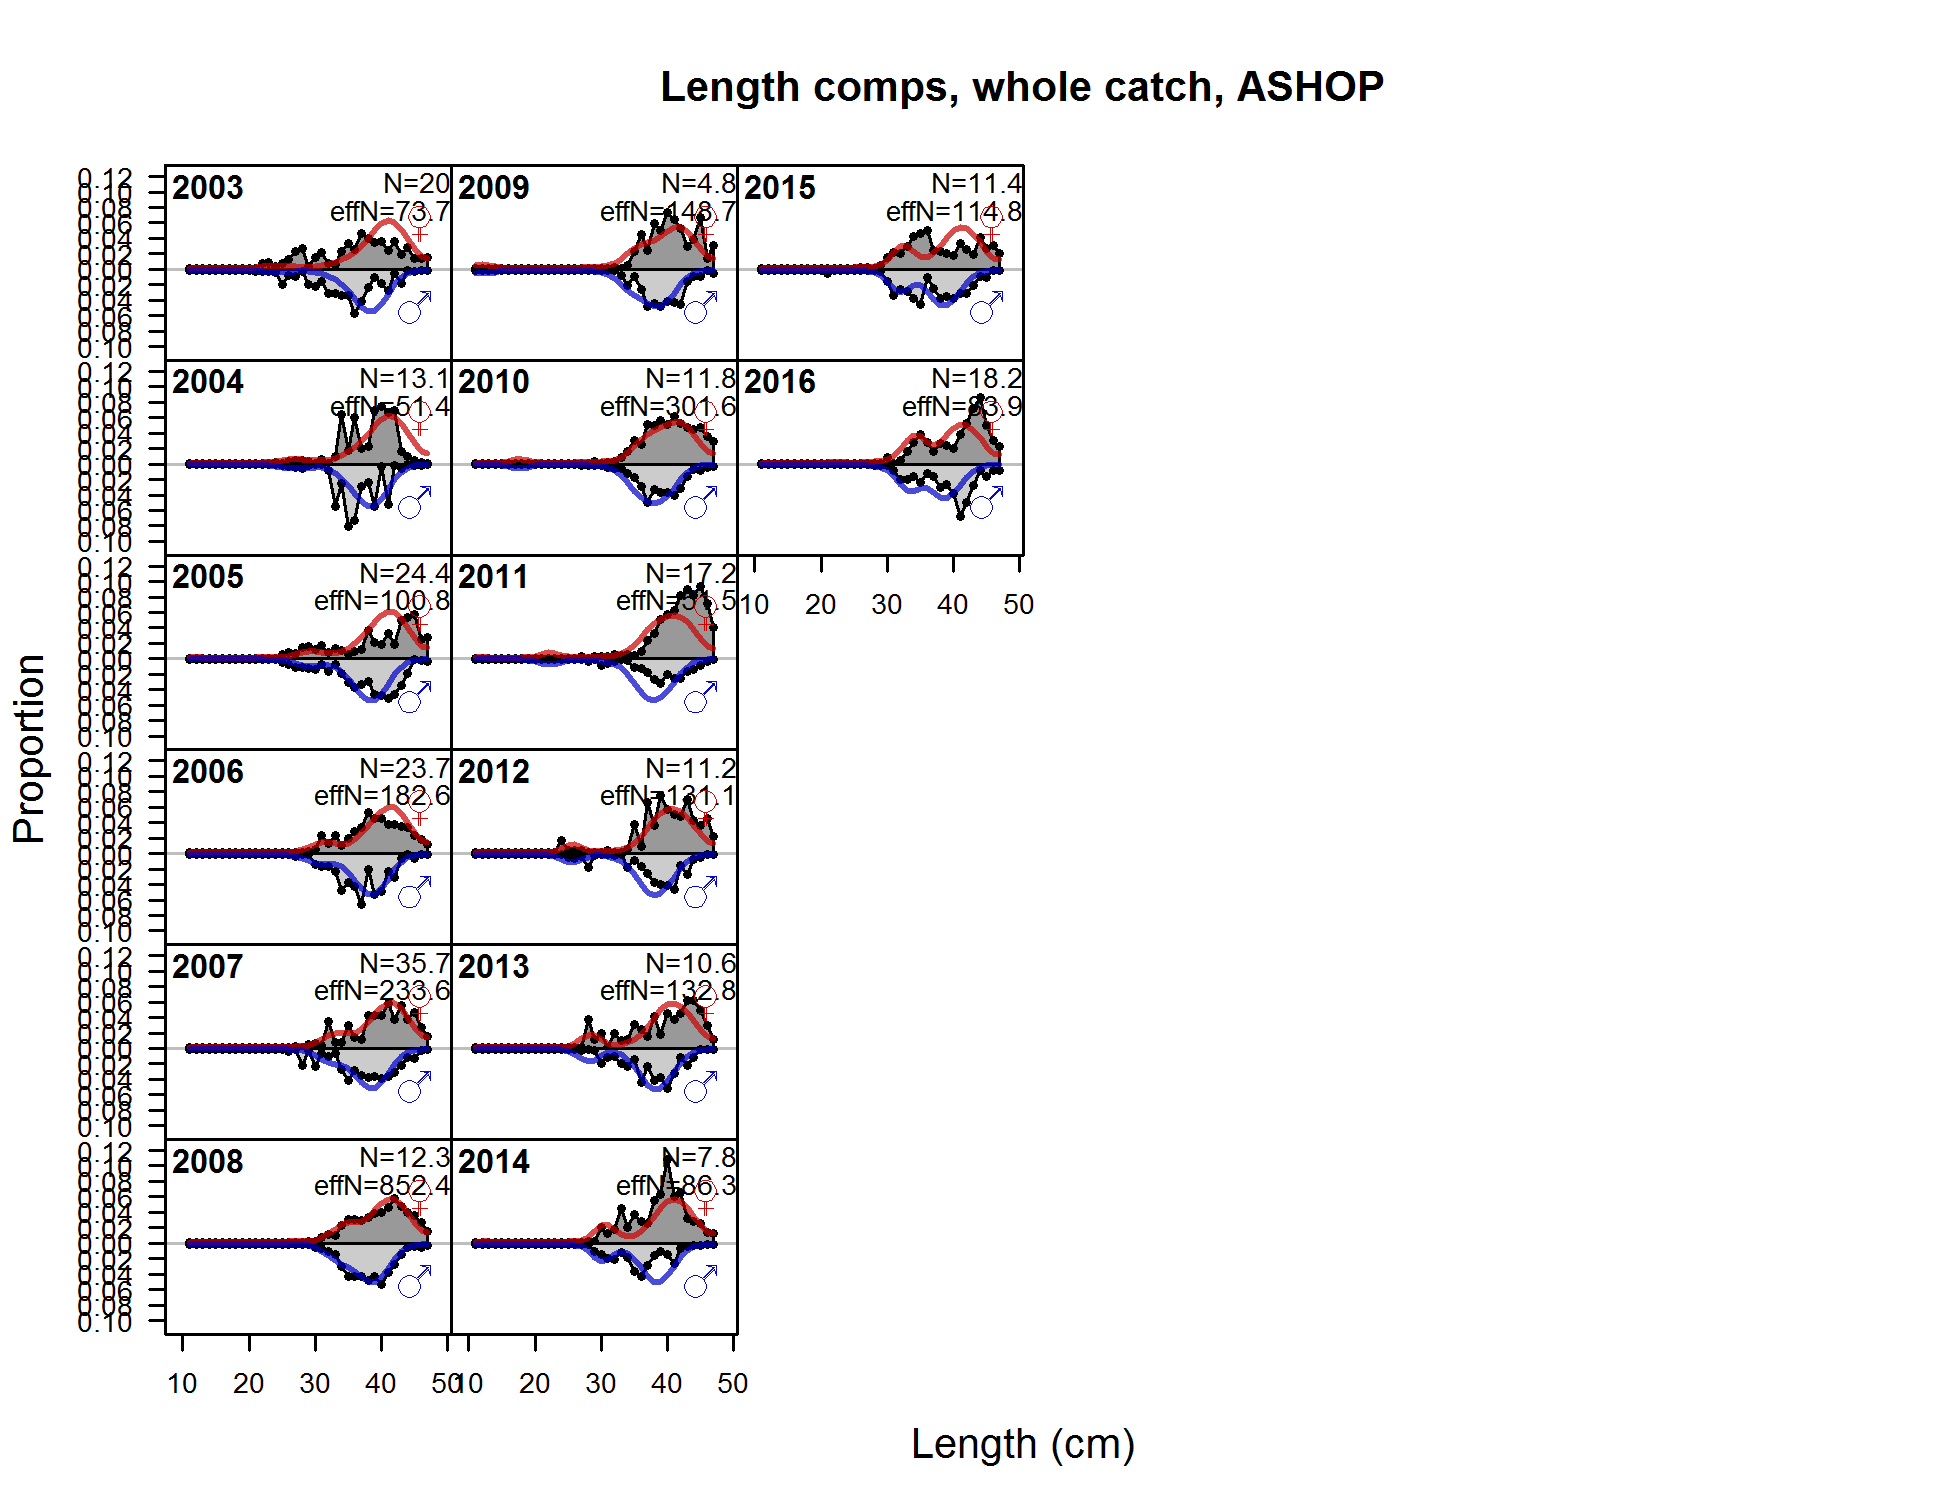
\includegraphics{./r4ss/plots_mod1/comp_lenfit_flt2mkt0.png}
\caption{length comps, whole catch, POP
\label{fig:mod1_9_comp_lenfit_flt2mkt0}}
\end{figure}

\begin{figure}
\centering
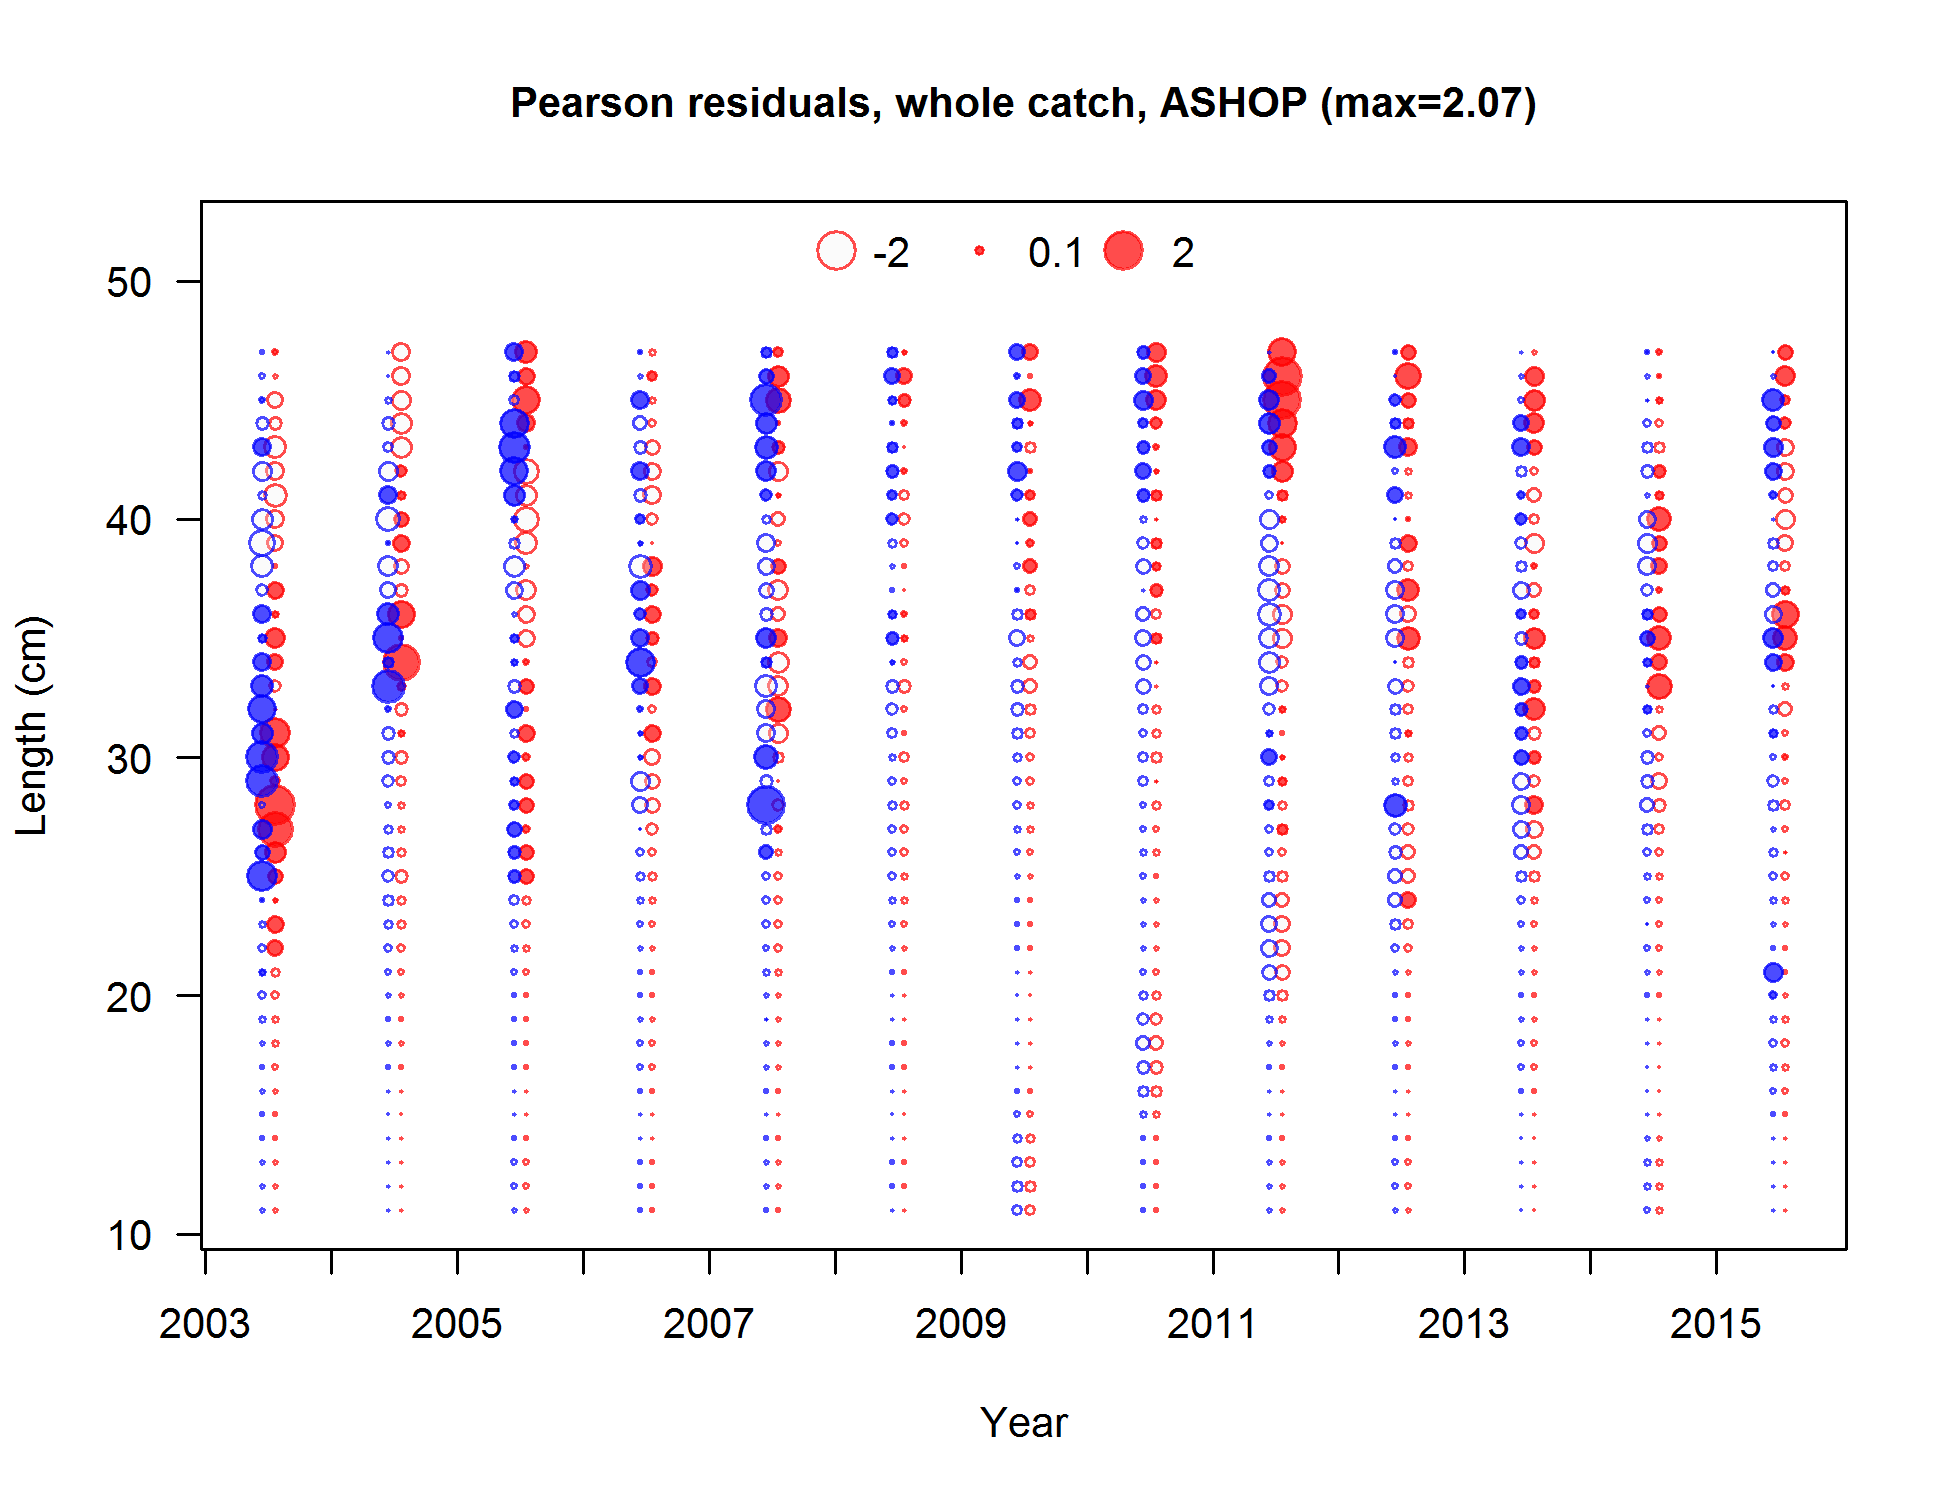
\includegraphics{./r4ss/plots_mod1/comp_lenfit_residsflt2mkt0.png}
\caption{Pearson residuals, whole catch, POP (max=3.28)\\
Closed bubbles are positive residuals (observed \textgreater{} expected)
and open bubbles are negative residuals (observed \textless{} expected).
\label{fig:mod1_10_comp_lenfit_residsflt2mkt0}}
\end{figure}

\FloatBarrier

\FloatBarrier

\FloatBarrier

\FloatBarrier

\FloatBarrier

\FloatBarrier

\FloatBarrier
<!-- ***********MODEL 2 REFERENCE POINTS FIGURES  -- IF NEEDED ************ -->

\newpage

\color{black}

\section*{References}\label{references}
\addcontentsline{toc}{section}{References}

\renewcommand{\thepage}{}

\hypertarget{refs}{}
\hypertarget{ref-bradburn_2003_2011}{}
Bradburn, M., Keller, A., and Horness, B. 2011. The 2003 to 2008 US West
Coast bottom trawl surveys of groundfish resources off Washington,
Oregon, and California: Estimates of distribution, abundance, length,
and age composition. US Department of Commerce, National Oceanic;
Atmospheric Administration, National Marine Fisheries Service.

\hypertarget{ref-dick_meta-analysis_2017}{}
Dick, E., Beyer, S., Mangel, M., and Ralston, S. 2017. A meta-analysis
of fecundity in rockfishes (genus \emph{Sebastes}). Fisheries Research
\textbf{187}: 73--85. doi:
\href{https://doi.org/10.1016/j.fishres.2016.11.009}{10.1016/j.fishres.2016.11.009}.

\hypertarget{ref-dick_modeling_2009}{}
Dick, E.J. 2009. Modeling the Reproductive Potential of Rockfishes
(\emph{Sebastes} Spp.). ProQuest. Available from
\url{http://books.google.com/books?hl=en\&lr=\&id=0d6-3rhfynkC\&oi=fnd\&pg=PR7\&dq=\%22Synthesis+of+findings+regarding+the+reproductive\%22+\%22C:+Linear+interpolation+algorithms\%22+\%22for+yellowtail+rockfish+(S.+flavidus)\%22+\%22greater+than+zero,+based+on+the+2-level+relative+fecundity\%22+\%22A:+Methods+for+data+recovery+from+published\%22+\&ots=NR0UylgymD\&sig=58IaN_a3pJeYTPYVmJ1NYMABmvE}
{[}accessed 27 February 2017{]}.

\hypertarget{ref-gunderson_population_1977}{}
Gunderson, D.R. 1977. Population biology of Pacific ocean perch,
\emph{Sebastes alutus}, stocks in the WashingtonQueen Charlotte Sound
region and their response to fishing. Fishery Bulletin \textbf{75}:
369--403. Available from
\url{http://fishbull.noaa.gov/75-2/gunderson.pdf} {[}accessed 27
February 2017{]}.

\hypertarget{ref-gunderson_results_1978}{}
Gunderson, D.R. 1978. Results of cohort analysis for Pacific ocean perch
stocks off British Columbia, Washington, and Oregon and an evaluation of
alternative rebuilding strategies for these stocks. Pacific Fishery
Management Council, 7700 Ambassador Place NE, Suite 200, Portland, OR
97220.

\hypertarget{ref-gunderson_distribution_1980}{}
Gunderson, D.R., and Sample, T.M. 1980. Distribution and abundance of
rockfish off Washington, Oregon and California during 1977. Northwest;
Alaska Fisheries Center, National Marine Fisheries Service. Available
from \url{http://spo.nmfs.noaa.gov/mfr423-4/mfr423-42.pdf} {[}accessed
28 February 2017{]}.

\hypertarget{ref-gunderson_status_1977}{}
Gunderson, D.R., Westrheim, S., Demory, R., and Fraidenburg, M. 1977.
The status of Pacific ocean perch (\emph{Sebastes alutus}) stocks off
British Columbia, Washington, and Oregon in 1974.

\hypertarget{ref-hamel_method_2015}{}
Hamel, O.S. 2015. A method for calculating a meta-analytical prior for
the natural mortality rate using multiple life history correlates. ICES
Journal of Marine Science: Journal du Conseil \textbf{72}(1): 62--69.
doi:
\href{https://doi.org/10.1093/icesjms/fsu131}{10.1093/icesjms/fsu131}.

\hypertarget{ref-karnowski_historical_2014}{}
Karnowski, M., Gertseva, V., and Stephens, A. 2014. Historical
Reconstruction of Oregon's Commercial Fisheries Landings. Oregon
Department of Fish; Wildlife, Salem, OR.

\hypertarget{ref-methot_stock_2013}{}
Methot, R.D., and Wetzel, C.R. 2013. Stock synthesis: A biological and
statistical framework for fish stock assessment and fishery management.
Fisheries Research \textbf{142}: 86--99. doi:
\href{https://doi.org/10.1016/j.fishres.2012.10.012}{10.1016/j.fishres.2012.10.012}.

\hypertarget{ref-pikitch_evaluation_1988}{}
Pikitch, E.K., Erickson, D.L., and Wallace, J.R. 1988. An evaluation of
the effectiveness of trip limits as a management tool. Northwest; Alaska
Fisheries Center, National Marine Fisheries Service NWAFC Processed
Report. Available from
\url{https://www.afsc.noaa.gov/Publications/ProcRpt/PR1988-27.pdf}
{[}accessed 28 February 2017{]}.

\hypertarget{ref-ralston_documentation_2010}{}
Ralston, S., Pearson, D.E., Field, J.C., and Key, M. 2010. Documentation
of the California catch reconstruction project. US Department of
Commerce, National Oceanic; Atmospheric Adminstration, National Marine.

\hypertarget{ref-rogers_species_2003}{}
Rogers, J. 2003. Species allocation of \emph{Sebastes} and
\emph{Sebastolobus} species caught by foreign countries off Washington,
Oregon, and California, U.S.A. in 1965-1976. Unpublished document.

\hypertarget{ref-rogers_numerical_1992}{}
Rogers, J.B., and Pikitch, E.K. 1992. Numerical definition of groundfish
assemblages caught off the coasts of Oregon and Washington using
commercial fishing strategies. Canadian Journal of Fisheries and Aquatic
Sciences \textbf{49}(12): 2648--2656. Available from
\url{http://www.nrcresearchpress.com/doi/abs/10.1139/f92-293}
{[}accessed 9 March 2017{]}.

\hypertarget{ref-seeb_genetic_1988}{}
Seeb, L.W., and Gunderson, D.R. 1988. Genetic variation and population
structure of Pacific ocean perch (\emph{Sebastes alutus}). Canadian
Journal of Fisheries and Aquatic Sciences \textbf{45}(1): 78--88.
Available from
\url{http://www.nrcresearchpress.com/doi/abs/10.1139/f88-010}
{[}accessed 28 February 2017{]}.

\hypertarget{ref-weinberg_estimation_2002}{}
Weinberg, J.R., Rago, P.J., Wakefield, W.W., and Keith, C. 2002.
Estimation of tow distance and spatial heterogeneity using data from
inclinometer sensors: An example using a clam survey dredge. Fisheries
Research \textbf{55}(1--3): 49--61. doi:
\href{https://doi.org/10.1016/S0165-7836(01)00292-2}{10.1016/S0165-7836(01)00292-2}.

\hypertarget{ref-wilkins_condition_1983}{}
Wilkins, M., and Golden, J. 1983. Condition of the Pacific ocean perch
resource off Washington and Oregon during 1979: Results of a cooperative
trawl survey. North American Journal of Fisheries Management \textbf{3}:
103--122.

\hypertarget{ref-withler_co-existing_2001}{}
Withler, R., Beacham, T., Schulze, A., Richards, L., and Miller, K.
2001. Co-existing populations of Pacific ocean perch, Sebastes alutus ,
in Queen Charlotte Sound, British Columbia. Marine Biology
\textbf{139}(1): 1--12. doi:
\href{https://doi.org/10.1007/s002270100560}{10.1007/s002270100560}.

\hypertarget{ref-zimmermann_influence_2003}{}
Zimmermann, M., Wilkins, M., Weinberg, K., Lauth, R., and Shaw, F. 2003.
Influence of improved performance monitoring on the consistency of a
bottom trawl survey. ICES Journal of Marine Science \textbf{60}(4):
818--826. doi:
\href{https://doi.org/10.1016/S1054-3139(03)00043-2}{10.1016/S1054-3139(03)00043-2}.

\end{document}
